% ------------------------------------------------------------
% LaTeX Template für die DHBW zum Schnellstart!
% Original: https://github.wdf.sap.corp/vtgermany/LaTeX-Template-DHBW
% ------------------------------------------------------------
% ---- Präambel mit Angaben zum Dokument
\documentclass[
	fontsize=12pt,           % Leitlinien sprechen von Schriftgröße 12.
	paper=A4,
	twoside=false,
	listof=totoc,            % Tabellen- und Abbildungsverzeichnis ins Inhaltsverzeichnis
	bibliography=totoc,      % Literaturverzeichnis ins Inhaltsverzeichnis aufnehmen
	titlepage,               % Titlepage-Umgebung anstatt \maketitle
	headsepline,             % horizontale Linie unter Kolumnentitel
	abstract,              % Überschrift einschalten, Abstract muss in {abstract}-Umgebung stehen
]{scrreprt}                  % Verwendung von KOMA-Report
\usepackage[utf8]{inputenc}  % UTF8 Encoding einschalten
\usepackage[ngerman]{babel}  % Neue deutsche Rechtschreibung
\usepackage[T1]{fontenc}     % Ausgabe von westeuropäischen Zeichen (auch Umlaute)
\usepackage{microtype}       % Trennung von Wörtern wird besser umgesetzt
\usepackage{lmodern}         % Nicht-gerasterte Schriftarten (bei MikTeX erforderlich)
\usepackage{graphicx}        % Einbinden von Grafiken erlauben
\usepackage{wrapfig}         % Grafiken fließend im Text
\usepackage{setspace}        % Zeilenabstand \singlespacing, \onehalfspaceing, \doublespacing
\usepackage[dvipsnames]{xcolor}
\usepackage{multicol}

\usepackage[
	%showframe,                % Ränder anzeigen lassen
	left=2.7cm, right=2.5cm,
	top=2.5cm,  bottom=2.5cm,
	includeheadfoot
]{geometry}                      % Seitenlayout einstellen
\usepackage{scrlayer-scrpage}    % Gestaltung von Fuß- und Kopfzeilen
\usepackage{acronym}             % Abkürzungen, Abkürzungsverzeichnis
\usepackage{titletoc}            % Anpassungen am Inhaltsverzeichnis
\contentsmargin{0.75cm}          % Abstand im Inhaltsverzeichnis zw. Punkt und Seitenzahl
\usepackage[                     % Klickbare Links (enth. auch "nameref", "url" Package)
  hidelinks,                     % Blende die "URL Boxen" aus.
  breaklinks=true                % Breche zu lange URLs am Zeilenende um
]{hyperref}
\usepackage[hypcap=true]{caption}% Anker Anpassung für Referenzen
\urlstyle{same}                  % Aktuelle Schrift auch für URLs
% Anpassung von autoref für Gleichungen (ergänzt runde Klammern) und Algorithm.
% Anstatt "Listing" kann auch z.B. "Code-Ausschnitt" verwendet werden. Dies sollte
% jedoch synchron gehalten werden mit \lstlistingname (siehe weiter unten).
\addto\extrasngerman{%
	\def\equationautorefname~#1\null{Gleichung~(#1)\null}
	\def\lstnumberautorefname{Zeile}
	\def\lstlistingautorefname{Listing}
	\def\algorithmautorefname{Algorithmus}
	% Damit einheitlich "Abschnitt 1.2[.3]" verwendet wird und nicht "Unterabschnitt 1.2.3"
	% \def\subsectionautorefname{Abschnitt}
}

% ---- Abstand verkleinern von der Überschrift 
\renewcommand*{\chapterheadstartvskip}{\vspace*{.5\baselineskip}}

% Hierdurch werden Schusterjungen und Hurenkinder vermieden, d.h. einzelne Wörter
% auf der nächsten Seite oder in einer einzigen Zeile.
% LaTeX kann diese dennoch erzeugen, falls das Layout ansonsten nicht umsetzbar ist.
% Diese Werte sind aber gute Startwerte.
\widowpenalty10000
\clubpenalty10000

% ---- Für das Quellenverzeichnis
\usepackage[
	backend = biber,                % Verweis auf biber
	language = auto,
	style = numeric,                % Nummerierung der Quellen mit Zahlen
	sorting = none,                 % none = Sortierung nach der Erscheinung im Dokument
	sortcites = true,               % Sortiert die Quellen innerhalb eines cite-Befehls
	block = space,                  % Extra Leerzeichen zwischen Blocks
	hyperref = true,                % Links sind klickbar auch in der Quelle
	%backref = true,                % Referenz, auf den Text an die zitierte Stelle
	bibencoding = auto,
	giveninits = true,              % Vornamen werden abgekürzt
	doi=false,                      % DOI nicht anzeigen
	isbn=false,                     % ISBN nicht anzeigen
    alldates=short                  % Datum immer als DD.MM.YYYY anzeigen
]{biblatex}
\addbibresource{Inhalt/literatur.bib}
\setcounter{biburlnumpenalty}{3000}     % Umbruchgrenze für Zahlen
\setcounter{biburlucpenalty}{6000}      % Umbruchgrenze für Großbuchstaben
\setcounter{biburllcpenalty}{9000}      % Umbruchgrenze für Kleinbuchstaben
\DeclareNameAlias{default}{family-given}  % Nachname vor dem Vornamen
\AtBeginBibliography{\renewcommand{\multinamedelim}{\addslash\space
}\renewcommand{\finalnamedelim}{\multinamedelim}}  % Schrägstrich zwischen den Autorennamen
\DefineBibliographyStrings{german}{
  urlseen = {Einsichtnahme:},                      % Ändern des Titels von "besucht am"
}
\usepackage[babel,german=quotes]{csquotes}         % Deutsche Anführungszeichen + Zitate


% ---- Für Mathevorlage
\usepackage{amsmath}    % Erweiterung vom Mathe-Satz
\usepackage{amssymb}    % Lädt amsfonts und weitere Symbole
\usepackage{MnSymbol}   % Für Symbole, die in amssymb nicht enthalten sind.


% ---- Für Quellcodevorlage
\usepackage{scrhack}                    % Hack zur Verw. von listings in KOMA-Script
\usepackage{listings}                   % Darstellung von Quellcode
\usepackage{xcolor}                     % Einfache Verwendung von Farben
% -- Eigene Farben für den Quellcode
\definecolor{JavaLila}{rgb}{0.4,0.1,0.4}
\definecolor{JavaGruen}{rgb}{0.3,0.5,0.4}
\definecolor{JavaBlau}{rgb}{0.0,0.0,1.0}
\definecolor{ABAPKeywordsBlue}{HTML}{6000ff}
\definecolor{ABAPCommentGrey}{HTML}{808080}
\definecolor{ABAPStringGreen}{HTML}{4da619}
\definecolor{PyKeywordsBlue}{HTML}{0000AC}
\definecolor{PyCommentGrey}{HTML}{808080}
\definecolor{PyStringGreen}{HTML}{008080}
% -- Farben für ABAP CDS
\definecolor{CDSString}{HTML}{FF8C00}
\definecolor{CDSKeywords}{HTML}{6000ff}
\definecolor{CDSAnnotation}{HTML}{00BFFF}
\definecolor{CDSComment}{HTML}{808080}
\definecolor{CDSFunc}{HTML}{FF0000}

% -- Default Listing-Styles

\lstset{
	% Das Paket "listings" kann kein UTF-8. Deswegen werden hier 
	% die häufigsten Zeichen definiert (ä,ö,ü,...)
	literate=%
		{á}{{\'a}}1 {é}{{\'e}}1 {í}{{\'i}}1 {ó}{{\'o}}1 {ú}{{\'u}}1
		{Á}{{\'A}}1 {É}{{\'E}}1 {Í}{{\'I}}1 {Ó}{{\'O}}1 {Ú}{{\'U}}1
		{à}{{\`a}}1 {è}{{\`e}}1 {ì}{{\`i}}1 {ò}{{\`o}}1 {ù}{{\`u}}1
		{À}{{\`A}}1 {È}{{\'E}}1 {Ì}{{\`I}}1 {Ò}{{\`O}}1 {Ù}{{\`U}}1
		{ä}{{\"a}}1 {ë}{{\"e}}1 {ï}{{\"i}}1 {ö}{{\"o}}1 {ü}{{\"u}}1
		{Ä}{{\"A}}1 {Ë}{{\"E}}1 {Ï}{{\"I}}1 {Ö}{{\"O}}1 {Ü}{{\"U}}1
		{â}{{\^a}}1 {ê}{{\^e}}1 {î}{{\^i}}1 {ô}{{\^o}}1 {û}{{\^u}}1
		{Â}{{\^A}}1 {Ê}{{\^E}}1 {Î}{{\^I}}1 {Ô}{{\^O}}1 {Û}{{\^U}}1
		{œ}{{\oe}}1 {Œ}{{\OE}}1 {æ}{{\ae}}1 {Æ}{{\AE}}1 {ß}{{\ss}}1
		{ű}{{\H{u}}}1 {Ű}{{\H{U}}}1 {ő}{{\H{o}}}1 {Ő}{{\H{O}}}1
		{ç}{{\c c}}1 {Ç}{{\c C}}1 {ø}{{\o}}1 {å}{{\r a}}1 {Å}{{\r A}}1
		{€}{{\euro}}1 {£}{{\pounds}}1 {«}{{\guillemotleft}}1
		{»}{{\guillemotright}}1 {ñ}{{\~n}}1 {Ñ}{{\~N}}1 {¿}{{?`}}1,
	breaklines=true,        % Breche lange Zeilen um 
	breakatwhitespace=true, % Wenn möglich, bei Leerzeichen umbrechen
	% Symbol für Zeilenumbruch einfügen
	prebreak=\raisebox{0ex}[0ex][0ex]{\ensuremath{\rhookswarrow}},
	postbreak=\raisebox{0ex}[0ex][0ex]{\ensuremath{\rcurvearrowse\space}},
	tabsize=4,                                 % Setze die Breite eines Tabs
	basicstyle=\ttfamily\small,                % Grundsätzlicher Schriftstyle
	columns=fixed,                             % Besseres Schriftbild
	numbers=left,                              % Nummerierung der Zeilen
	%frame=single,                             % Umrandung des Codes
	showstringspaces=false,                    % Keine Leerzeichen hervorheben
	keywordstyle=\color{blue},
	ndkeywordstyle=\bfseries\color{darkgray},
	identifierstyle=\color{black},
	commentstyle=\itshape\color{JavaGruen},   % Kommentare in eigener Farbe
	stringstyle=\color{JavaBlau},             % Strings in eigener Farbe,
	captionpos=b,                             % Bild*unter*schrift
	xleftmargin=5.0ex
}

% ---- Eigener JAVA-Style für den Quellcode
\renewcommand{\ttdefault}{pcr}               % Schriftart, welche auch fett beinhaltet
\lstdefinestyle{EigenerJavaStyle}{
	language=Java,                             % Syntax Highlighting für Java
	%frame=single,                             % Umrandung des Codes
	keywordstyle=\bfseries\color{JavaLila},    % Keywords in eigener Farbe und fett
	commentstyle=\itshape\color{JavaGruen},    % Kommentare in eigener Farbe und italic
	stringstyle=\color{JavaBlau}               % Strings in eigener Farbe
}

% ---- Eigener ABAP-Style für den Quellcode
\renewcommand{\ttdefault}{pcr}
\lstdefinestyle{EigenerABAPStyle}{
	language=[R/3 6.10]ABAP,
	morestring=[b]\|,                          % Für Pipe-Strings
	morestring=[b]\`,                          % für Backtick-Strings
	keywordstyle=\bfseries\color{ABAPKeywordsBlue},
	commentstyle=\itshape\color{ABAPCommentGrey},
	stringstyle=\color{ABAPStringGreen},
	tabsize=2,
	morekeywords={
		types,
		@data,
		as,
		lower,
		start,
		selection,
		order,
		by,
		inner,
		join,
		key,
		end,
		cast
	}
}

% ---- Eigener Python-Style für den Quellcode
\renewcommand{\ttdefault}{pcr}
\lstdefinestyle{EigenerPythonStyle}{
	language=Python,
	columns=flexible,
	keywordstyle=\bfseries\color{PyKeywordsBlue},
	commentstyle=\itshape\color{PyCommentGrey},
	stringstyle=\color{PyStringGreen}
}

%----- ABAP-CDS-View language
\lstdefinelanguage{ABAPCDS}{
	sensitive=false,
	%Keywords
	morekeywords={define,
		view,
		as,
		select,
		from,
		inner,
		join,
		on,
		key,
		case,
		when,
		then,
		else,
		end,
		true,
		false,
		cast,
		where,
		and,
		distinct,
		group,
		by,
		having,
		min,
		sum,
		max,
		count,
		avg
	},
	%Methoden
	morekeywords=[2]{
		div,
		currency\_conversion,
		dats\_days\_between,
		concat\_with\_space,
		dats\_add_days,
		dats\_is\_valid,
		dats\_add\_months,
		unit\_conversion,
		division,
		mod,
		abs,
		floor,
		ceil,
		round,
		concat,
		replace,
		substring,
		left,
		right,
		length
	},
	morecomment=[s][\color{CDSAnnotation}]{@}{:},
	morecomment=[l][\itshape\color{CDSComment}]{//},
	morecomment=[s][\itshape\color{CDSComment}]{/*}{*/},
	morestring=[b][\color{CDSString}]',
	keywordstyle=\bfseries\color{CDSKeywords},
	keywordstyle=[2]\color{CDSFunc}
}

\definecolor{comment}{HTML}{606060}
\definecolor{string}{HTML}{6060FF}
\definecolor{keywords}{HTML}{606000}

% \lstset{
% 	breaklines=true,
% 	breakatwhitespace=true,
% 	prebreak=\raisebox{0ex}[0ex][0ex]{\ensuremath{\rhookswarrow}},
% 	postbreak=\raisebox{0ex}[0ex][0ex]{\ensuremath{\rcurvearrowse\space}},
% 	columns=fixed,
% 	numbers=left,
% 	numberblanklines=false
% 	basicstyle=\small,
% 	showstringspaces=false,
% 	keepspaces=true,
% 	literate=%
% 	{Ö}{{\"O}}1
% 	{Ä}{{\"A}}1
% 	{Ü}{{\"U}}1
% 	{ß}{{\ss}}1
% 	{ü}{{\"u}}1
% 	{ä}{{\"a}}1
% 	{ö}{{\"o}}1
% }

\lstdefinestyle{Pseudocode} {
	morekeywords={WENN, SOLANGE, ENDE, BEGINN, FUEHRE, AUS, SONST, GIB, UND, FUER, NICHT, SOBALD},
	morecomment=[l]{;},
	morecomment=[s]{/*}{*/},
	morestring=[b]\=,
	basicstyle=\ttfamily\small,
	keywordstyle=\bfseries\color{keywords},
	stringstyle=\color{string},
	commentstyle=\itshape\color{comment},
	xleftmargin=3.0ex
}

\lstdefinestyle{json-web-schnittstelle} {
	basicstyle=\ttfamily\small,
	numbers=none, 
	xleftmargin=0.2ex
}  % Weitere Details sind ausgelagert

\usepackage{algorithm}                  % Für Algorithmen-Umgebung (ähnlich wie lstlistings Umgebung)
\usepackage{algpseudocode}              % Für Pseudocode. Füge "[noend]" hinzu, wenn du kein "endif",
                                        % etc. haben willst.

\makeatletter                           % Sorgt dafür, dass man @ in Namen verwenden kann.
                                        % Ansonsten gibt es in der nächsten Zeile einen Compilefehler.
\renewcommand{\ALG@name}{Algorithmus}   % Umbenennen von "Algorithm" im Header der Listings.
\makeatother                            % Zeichen wieder zurücksetzen
\renewcommand{\lstlistingname}{Listing} % Erlaubt das Umbenennen von "Listing" in anderen Titel.

% ---- Tabellen
\usepackage{booktabs}  % Für schönere Tabellen. Enthält neue Befehle wie \midrule
\usepackage{multirow}  % Mehrzeilige Tabellen
\usepackage{siunitx}   % Für SI Einheiten und das Ausrichten Nachkommastellen
\sisetup{locale=DE, range-phrase={~bis~}, output-decimal-marker={,}} % Damit ein Komma und kein Punkt verwendet wird.
\usepackage{xfrac} % Für siunitx Option "fraction-function=\sfrac"

% ---- Für Definitionsboxen in der Einleitung
\usepackage{amsthm}                     % Liefert die Grundlagen für Theoreme
\usepackage[framemethod=tikz]{mdframed} % Boxen für die Umrandung
% ---- Definition für Highlight Boxen

% ---- Grundsätzliche Definition zum Style
\newtheoremstyle{defi}
  {\topsep}         % Abstand oben
  {\topsep}         % Abstand unten
  {\normalfont}     % Schrift des Bodys
  {0pt}             % Einschub der ersten Zeile
  {\bfseries}       % Darstellung von der Schrift in der Überschrift
  {:}               % Trennzeichen zwischen Überschrift und Body
  {.5em}            % Abstand nach dem Trennzeichen zum Body Text
  {\thmname{#3}}    % Name in eckigen Klammern
\theoremstyle{defi}

% ------ Definition zum Strich vor eines Texts
\newmdtheoremenv[
  hidealllines = true,       % Rahmen komplett ausblenden
  leftline = true,           % Linie links einschalten
  innertopmargin = 0pt,      % Abstand oben
  innerbottommargin = 4pt,   % Abstand unten
  innerrightmargin = 0pt,    % Abstand rechts
  linewidth = 3pt,           % Linienbreite
  linecolor = gray!40,       % Linienfarbe
]{defStrich}{Definition}     % Name der des formats "defStrich"

% ------ Definition zum Eck-Kasten um einen Text
\newmdtheoremenv[
  hidealllines = true,
  innertopmargin = 6pt,
  linecolor = gray!40,
  singleextra={              % Eck-Markierungen für die Definition
    \draw[line width=3pt,gray!50,line cap=rect] (O|-P) -- +(1cm,0pt);
    \draw[line width=3pt,gray!50,line cap=rect] (O|-P) -- +(0pt,-1cm);
    \draw[line width=3pt,gray!50,line cap=rect] (O-|P) -- +(-1cm,0pt);
    \draw[line width=3pt,gray!50,line cap=rect] (O-|P) -- +(0pt,1cm);
  }
]{defEckKasten}{Definition}  % Name der des formats "defEckKasten"  % Weitere Details sind ausgelagert

% ---- Für Todo Notes
\usepackage{todonotes}
\setlength {\marginparwidth }{2cm}      % Abstand für Todo Notizen

% ---- Für Enumerates
\usepackage{enumitem}

% ---- Für .svg Datein
\usepackage{svg}

% --- Für Images
\usepackage{float}

% ---- Elektronische Version oder Gedruckte Version?
% ---- Unterschied: Die elektronische Version enthält keinen Platzhalter für die Unterschrift
\usepackage{ifthen}
\newboolean{e-Abgabe}
\setboolean{e-Abgabe}{false}    % false=gedruckte Fassung

% ---- Persönlichen Daten:
\newcommand{\bearbeitende}{Andr\'{e} Trump und Erik Imgrund} % Alphabetisch nach Vornamen

% ---- Metainformation für das PDF Dokument
\hypersetup{
	pdftitle    = {Software-Engineering TINF19B1},
	pdfsubject  = {Programmentwurf Eventplaner},
	pdfauthor   = {\bearbeitende},
	%pdfkeywords = {Keywords angeben},
	pdfcreator  = {LaTeX},
	%pdfproducer = {in der Regel pdfTeX}
}

% ---- Definition der Kopf- und Fußzeilen
\clearscrheadfoot                               % Löschen von LaTeX Standard
\automark[section]{chapter}                     % Füllen von section und chapter
\renewcommand*{\chaptermarkformat}{}            % Entfernt die Kapitelnummer
\renewcommand*{\sectionmarkformat}{}            % Entfernt die Sectionnummer
% Angaben [für "plain"]{für "scrheadings"}
\ihead[]{Programmentwurf Eventplaner}                          % Kopfzeile links
\chead[]{}                                      % Kopfzeile mitte
\ohead[]{\rightmark}                            % Kopfzeile rechts
\ifoot[]{}                                      % Fußzeile links
\cfoot*{\sffamily\pagemark}                     % Fußzeile mitte
\ofoot[]{}                                      % Fußzeile rechts
\KOMAoptions{
   headsepline = 0.2pt,                         % Liniendicke Kopfzeile
   footsepline = false                          % Liniendicke Fußzeile
}

% ---- Hilfreiches
\newcommand{\zB}{z.\,B. }   % "z.B." mit kleinem Leeraum dazwischen (ohne wäre nicht korrekt)
\newcommand{\dash}{d.\,h. }

\newcommand{\code}[1]{\texttt{#1}} % Ist einfacher zu schreiben als ständig \texttt und erlaubt
                                   % Änderungen im Nachhinein, wenn man z.B. Inline-Code anders stylen möchte.

% ---- Silbentrennung (falls LaTeX defaults falsch / nicht gewünscht sind)
\hyphenation{HANA}         % anstatt HA-NA
\hyphenation{Graph-Script} % anstatt GraphS-cript

% ---- Beginn des Dokuments
\begin{document}
\setlength{\parindent}{0pt}              % Keine Paragraphen Einrückung.
                                         % Dafür haben wir den Abstand zwischen den Paragraphen.
\setcounter{secnumdepth}{2}              % Nummerierungstiefe fürs Inhaltsverzeichnis
\setcounter{tocdepth}{2}                 % Tiefe des Inhaltsverzeichnisses. Ggf. so anpassen,
                                         % dass das Verzeichnis auf eine Seite passt.
\sffamily                                % Serifenlose Schrift verwenden.

% ---- Vorspann
% ------ Titelseite
\singlespacing
\thispagestyle{empty}
\begin{titlepage}
\enlargethispage{4cm}

\begin{figure}           % Logo vom Ausbildungsbetrieb und der DHBW
	% \vspace*{-5mm} % Sollte dein Titel zu lang werden, kannst du mit diesem "Hack" 
	%                  den Inhalt der Seite nach oben schieben.
	\begin{minipage}{0.49\textwidth}
		\flushleft
		
\includegraphics[height=2.5cm]{Bilder/Logos/Carsharing.PNG} 
	\end{minipage}
	\hfill
	\begin{minipage}{0.49\textwidth}
		\flushright
		
\includegraphics[height=2.5cm]{Bilder/Logos/Logo_DHBW.pdf} 
	\end{minipage}
\end{figure} 
\vspace*{0.1cm}

\begin{center}
	\huge{\textbf{\titel}}\\[1.5cm]
	\Large{\textbf{\arbeit}}\\[0.5cm]
	\normalsize{im Rahmen der Prüfung zum\\[1ex] \textbf{Bachelor of Science (B.Sc.)}}\\[0.5cm]
	\Large{des Studienganges \studiengang}\\[1ex]
	\normalsize{an der Dualen Hochschule Baden-Württemberg Karlsruhe}\\[1cm]
	\normalsize{von}\\[1ex] \Large{\textbf{\autor}} \\[1cm]
\end{center}

\begin{center}
	\vfill
	\begin{tabular}{ll}
		Abgabedatum:                     & \abgabe \\[0.2cm]
		Bearbeitungszeitraum:            & \bearbeitungszeitraum \\[0.2cm]
		Kurs:            				 & \kurs \\[0.2cm]
		
		Gutachter der Dualen Hochschule: & \betreuerDhbw \\[2cm]
	\end{tabular} 
\end{center}
\end{titlepage}
  % Titelseite
\newcounter{savepage}
\pagenumbering{Roman}                    % Römische Seitenzahlen
\onehalfspacing


% ------ Inhaltsverzeichnis
\singlespacing
\tableofcontents

% ------ Verzeichnisse
\renewcommand*{\chapterpagestyle}{plain}
\pagestyle{plain}
\setcounter{savepage}{\value{page}}


% ---- Inhalt der Arbeit
\cleardoublepage
\pagenumbering{arabic}                  % Arabische Seitenzahlen für den Hauptteil
\setlength{\parskip}{0.5\baselineskip}  % Abstand zwischen Absätzen
\rmfamily
\renewcommand*{\chapterpagestyle}{scrheadings}
\pagestyle{scrheadings}
\singlespacing
\chapter{Aufgabenstellung}
\section{Einleitung}
Für unser sehr erfolgreiches Startup-Unternehmen im Bereich Event-Management benötigen wir ein neues Planungssystem, um alle Event-Daten noch besser und effizienter erfassen und verwalten zu können.

Dabei planen und veranstalten wir Events mit Teilnehmerzahlen bis ca. 1000 Personen (Kongresse, Hochzeiten, Empfänge, Vernissagen, Sportveranstaltungen, Wettbewerbe, Konzerte usw.). Die meisten Events führen wir für 50 - 100 Teilnehmer durch.

Bisher vor kurzem war es möglich, mit Hilfe von Excel die Planung und Verwaltung unserer Events durchzuführen, was durch die stark steigende Anzahl an Events nun nicht mehr auf Dauer realisierbar ist.

\section{Lastenheft}
\subsection{Zielsetzung}
Ziel des Entwicklungsauftrags ist eine Software für die Planung und Durchführung von Veranstaltungs-Events. Alle Daten sollen zentral gespeichert werden, da mehrere Benutzer gleichzeitig auf die Daten und Termine zugreifen werden.

Ein selektiver Import und Export von Daten über lesbare Dateien muss für Backups und zum Datenaustausch möglich sein.

Eine intuitive, leicht bedienbare Benutzeroberfläche setzen wir als selbstverständlich voraus. Es sollen keine besonderen Computerkenntnisse zur Bedienung der Software erforderlich sein. 
\subsection{Anwendungsbereiche}
Die Software soll ausschließlich für die Planung und Verwaltung von Events, Kunden, Ausrüstung, Locations und Angestellten und den damit direkt verbundenen Elementen verwendet werden. Sie soll im Alltag auf Laptops eingesetzt werden.
\subsection{Zielgruppen, Benutzerrollen und Verantwortlichkeiten}
Es soll verschiedene Benutzerrollen geben:
\begin{itemize}
    \item Organisatorinnen und Organisatoren pflegen die jeweiligen Event-Daten
    \item Beschaffungspersonal (besorgen und verwalten benötigte Utensilien, die mehrfach verwendet werden können). Es hat lesenden Zugriff auf von Organisatorinnen und Organisatoren freigegebene Teilevents. Sie können in Gruppen organisiert sein (d.h. es gibt eine/n Gruppenleiterin bzw. einen Gruppenleiter) für Aktionen, die nicht oder nur schwer allein zu realisieren sind. 
    \item Personalmitarbeiter pflegen Mitarbeiterdaten im System 
    \item Montageleiterinnen und Montageleiter (Leitung von Mitarbeitern für den Auf- und Abbau der benötigten Geräte, Bauten und Einrichtungen). Die Rolle soll lesenden Zugriff auf alle Daten haben, die in ihren Arbeitsbereich fallen.
    \item Eine hauptverantwortliche Person (Administrator) hat Vollzugriff auf sämtliche Daten, vor allem für deren Import und Export sowie deren Backup. 
\end{itemize}
\subsection{Zusammenspiel mit anderen Systemen}
Die Daten über die Angestellten (Gehälter bzw. Löhne, Steuern, Kranken- und Rentenversicherung usw.) werden separat durch ein vorhandenes Personalbuchhaltungsprogramm verwaltet und müssen hier nicht berücksichtigt werden. Die finanztechnischen Daten werden über unser vorhandenes Finanzsystem erfasst und müssen hier ebenfalls nicht berücksichtigt werden.

Eine Web-Seite über unser Unternehmen existiert bereits, Anfragen für die Durchführung von Events werden per E-Mail gestellt und ist von der neuen Software unabhängig.

In einer zweiten Ausbaustufe soll es möglich sein, dass das Beschaffungspersonal und die Montageleiter über das Internet (Handy, Tablet) erledigte Aufgaben „abhaken“ können. Diese Funktionalität wird jedoch in der ersten Ausbaustufe noch nicht benötigt, die Erledigung einzelner Teilaufgaben wird dann noch per Mail oder Telefonanruf mit den Organisatorinnen und Organisatoren erledigt.

Allerdings benötigen wir ein klares Konzept, wie diese Erweiterung realisiert werden soll. 

Möglichst alle Daten sollen vom alten in das neue System übertragen werden.
\subsection{Produktfunktionen}
\paragraph{/LF10/}
Der jeweilige Benutzer muss die Möglichkeit haben, über eine grafische Benutzeroberfläche alle für ihn relevanten Daten einfach und übersichtlich zu verwalten.
\paragraph{/LF20/}
Verwaltet werden sollen Events, die geplant und durchgeführt werden. Sie bestehen aus einzelnen Teilschritten (Teilevents), die parallel oder nacheinander ausgeführt werden können.

Jedes (Teil-)Event hat einen Start- und einen Ende-Termin, eine Bezeichnung (Name), Kontaktdaten (für Ansprechpersonen, z.B. Verwalter einer Location), eine Liste von benötigten Hilfsmitteln, eine Beschreibung, einen Status (erstellt, geplant, in Arbeit, fertig, usw.), die Möglichkeit, Kosten abzubilden sowie weitere Attribute.
\paragraph{/LF30/}
Hilfsmittel sind Tische, Stühle, Deko-Elemente (viele Varianten!), Gastronomie-Grills, u.v.m. Bei der Eintragung der Hilfsmittel soll jeweils die benötigte Anzahl angegeben werden können. Allen Hilfsmitteln müssen mehrere Termine zugeordnet werden können. Terminüberschneidungen müssen vermieden werden, um die Verfügbarkeit sicherzustellen.
\paragraph{/LF40/}
So genannte Event-Elemente sind:
\begin{itemize}
    \item Catering
    \item Musik (Bands, Musikerinnen und Musiker, DJs usw.)
    \item Multimedia (Beschallung, Anlagen (Verstärker, Boxen, Mikrofone, ...)) 
    \item Personen (z.B. Entertainer, Pastor für Trauungen, Redner, Clowns, Comedians, Musiker (Bands) etc.)
    \item Location (Veranstaltungsort, d.h. Lage, Adresse, Größe, u.v.m.)
\end{itemize}

Alle Event-Elemente können wiederum aufgeteilt werden (Teil-Event oder Teil-Element mit Start- und Ende-Termin sowie einen möglichen Verweis auf eine Firma incl. Ansprechpartner und evtl. Angebot, Vertragsdetails usw.)
\paragraph{/LF50/}
Für die Organisatorinnen und Organisatoren soll es möglich sein, Mails an Personen und Mitarbeiter mit Informationen über den Teilevent aus dem System heraus zu versenden. Dazu sollen die Kontaktdaten verwendet werden, die bei den Events eingetragen sind.
\paragraph{/LF60/}
Alle Angestellten müssen verwaltet werden. Jedem Teil-Event können die gewünschten Angestellten zugeordnet werden
\paragraph{/LF70/}
Zur einfacheren Eingabe der Daten soll es Auswahllisten für deren Eigenschaften geben, wo immer es möglich ist. Die Auswahllisten sollen auf einfache Weise erweiterbar sein.
\paragraph{/LF80/}
Sämtlichen Elementen sollen mehrere Bilder mit Titel zugeordnet werden können, die zentral auf einem Verzeichnis liegen sollen
\paragraph{/LF90/}
Bei der Zuordnung von eingetragenen Hilfsmitteln zu Teil-Events muss darauf geachtet werden, ob die Hilfsmittel im gewünschten Zeitraum verfügbar sind.
\paragraph{/LF100/}
Es muss möglich sein, alle Teil-Events für ausgewählte Angestellte in einer Auflistung anzeigen zu lassen.
\subsection{Produktdaten}
\paragraph{/LD10/}
Die Daten sollen in einer zentralen Datenbasis (lesbare Dateien) abgespeichert werden.
\subsection{Produktleistungen}
\paragraph{/LL10/}
Die Anzahl der zu verwaltenden Elemente wird auf ca. 50.000 geschätzt.
\paragraph{/LL20/}
Um bei HW- und SW-Anschaffungen und -neuerungen flexibel zu bleiben, ist auf Plattformunabhängigkeit besonders zu achten.
\subsection{Qualitätsanforderungen}
\begin{tabular}{| l | c | c | c | c |}
    \hline
    Produktqualität & sehr gut & gut & normal & nicht relevant \\
    \hline
    Funktionalität & x & & & \\
    \hline
    Zuverlässigkeit & & x & & \\
    \hline
    Effizienz & & x & & \\
    \hline
    Benutzbarkeit & x & & & \\
    \hline
    Wartbarkeit & & & x & \\
    \hline
    Übertragbarkeit & & & x & \\
    \hline
\end{tabular}
\section{Aufgaben}
Einzelne Lastenheftpunkte sind bewusst offengehalten. Denken Sie darüber nach, welche Informationen zusätzlich sinnvoll oder auch notwendig sind. Recherchieren Sie evtl. nach einzelnen Zusammenhängen im Internet.
\subsection{Analyse}
Für die Analyse sind zu erstellen:
\begin{itemize}
    \item Analyse des Lastenhefts (Fragen und Antworten). 
    \item Ein Use-Case-Diagramm der gesamten Anwendung incl. Beschreibung.
    \item Eine Verfeinerung des Use-Case-Diagramms incl. Beschreibung. (nach Absprache)
    \item Ein Analyse-Klassendiagramm incl. Beschreibung (Untersuchen Sie dabei den Einsatz geeigneter Analysemuster)
    \item Einfache GUI-Skizzen (Mockups) von mindestens zwei wesentlichen GUI-Komponenten (Hauptseite, Tabs, etc.). Die Skizzen können mit einem einfachen Grafikprogramm erstellt werden. Auch sorgfältige Handzeichnungen sind erlaubt. Keine Login-GUI skizzieren!    
\end{itemize}
\subsection{Sequenzdiagramm und Aktivitätsdiagramm}
Erstellen Sie ein Sequenzdiagramm und ein Aktivitätsdiagramm (incl. Beschreibung) für folgende Szenarios (ein AD für das eine Szenario, ein SD für das andere Szenario):
\begin{itemize}
    \item Die Aktion „Event anlegen“ durchführen. Ausgehend von einem neuen Event und leerer Datenbasis werden dessen gesamte Daten erfasst und in das System eingetragen. (dies wird als Gebrauchsanweisung für die Evaluation Ihrer Implementierung dienen)
    \item Die Aktionen „Event durchführen“ anhand eines praktischen Beispiels (Kongress, Abschlussfeier, Konzert o.ä.) 
\end{itemize}
Die Bewertung Ihrer Diagramme erfolgt auf der Basis der Nutzung der UML-Elemente, auf Ihrer Kreativität sowie dem Detaillierungsgrad des jeweiligen Diagramms.

Fassen Sie bei beiden Diagrammen die Eingabe aller primitiven Attribute eines Elements (Float, String, Integer, …) in einer einzigen Aktion zusammen (z.B. „Attribute eintragen“).

Für das Sequenzdiagramm ist das gewählte Szenario ausführlich zu entwickeln (idealerweise mit Pseudocode). Es sind sämtliche referenzierten Elemente zu berücksichtigen, die zugeordnet werden können. 

In allen Fällen wird eine (noch) leere Datenbasis angenommen. Denken Sie an geeignete Diagrammverfeinerungen. 

\subsection{Entwurf}
Abzuliefern sind hier (alle Diagramme und GUIs jeweils mit Beschreibung):
\begin{itemize}
    \item Entwurfsklassendiagramm (Untersuchen Sie dabei den Einsatz geeigneter Entwurfsmuster)
\item GUI-Modellierung:

Es ist das Kommunikationsschema eines Teils der während der Analyse skizzierten GUI mit UML zu modellieren. Die Anwendung selbst soll dabei nach dem einfachen Model-View-Control-Muster aufgebaut sein. Dazu sind mindestens ein Controller, die erforderlichen Modellklassen sowie eine unabhängige GUI (View) erforderlich.

Die meisten GUI-Elemente werden über eine einfache kleine Java-Bibliothek zur Verfügung gestellt (swe-utils.jar), deren GUI-Komponenten in das Klassendiagramm zu integrieren sind, wenn sie verwendet werden.

Die GUI-Modellierung kann in einem separaten Diagramm mit den relevanten (gewählten bzw. benötigten) Modellklassen erfolgen, falls das Entwurfsklassendiagramm sonst zu komplex werden würde. 
\end{itemize}
\subsection{Implementierung}
Es ist eine einfache Java-Applikation zu implementieren, die es ermöglicht, Museumsdaten anzulegen, zu ändern und zu löschen. 

Zur Realisierung wird die oben bei der Entwurfsaufgabe erwähnte Java-Bibliothek zur Verfügung gestellt (swe-utils.jar), die neben mehreren GUI-Komponenten einen CSVReader, einen CSVWriter sowie mehrere Interfaces bereitstellt (in den Packages event und model).

Daneben ist eine Mini-Test-Applikation gegeben, die die Funktionsfähigkeit der GUI-Komponenten demonstriert (Start mit java -jar swe-utils.jar). Details sind der Java-Dokumentation der Bibliothek zu entnehmen.

Zur leichteren und zukunftssicheren Evaluation Ihres Programmentwurfs soll die Java-Applikation als eine Desktop-Applikation mit CSV-Dateien (alternativ XML oder JSON) als zentrale Datenbasis realisiert werden, die von beliebigen Rechnern aus gestartet wird. Dabei sind mehrere Dateien analog zu Datenbanktabellen zu erzeugen.
\subsubsection*{Einzelne Aufgaben}
\begin{itemize}
    \item Hauptaufgabe ist die Realisierung einer MVC-Applikation mithilfe des Observer-Patterns entsprechend des vorgegebenen GUI-Entwurfs und der gegebenen Java-Bibliothek.
    \item Die Erzeugung der Instanzen soll in einer Entity-Factory erfolgen und zur Verwaltung der Instanzen ist ein Entity-Manager zu realisieren (beides siehe Vorlesung).
    \item Beim Anlegen eines Events muss für die Zuordnung von Hilfsmitteln sichergestellt sein, dass es keine zeitlichen Überschneidungen gibt (LF90).
    \item Es muss eine ausführbare JAR-Datei abgegeben werden, die mit 
    
    \code{java -jar SWE-PE-2021\_Eventplaner\_<name1>\_<name2>.jar OPTIONEN} gestartet werden kann. Hierfür ist ein BASH-Skript namens startApp zu erstellen.
    \item Geprüft wird das Anlegen eines Events mit der Zuordnung aller zugehörigen Elemente. Nach dem Anlegen wird die Applikation erneut gestartet und geprüft, ob alle Daten korrekt abgespeichert und beim Laden wieder zugeordnet werden. 
\end{itemize}
\subsubsection*{Verwendung von CSV-Dateien:}
\begin{itemize}
    \item Die Daten sollen in CSV-Dateien vorliegen und können mittels den gegebenen Bibliotheksklassen CSVReader und CSVWriter gelesen bzw. beschrieben werden. Zur Vereinfachung können die Daten jeweils komplett geschrieben werden. 
    \item Abgegeben werden soll ein ZIP-File (oder TAR-File) mit allen Java- und CSV-Dateien (letztere gesammelt in einem eigenen Verzeichnis): 
    
    \enquote{SWE-PE-2021\_Eventplaner\_<n1>\_<n2>.zip} (tar oder tar.z) 
    \item Als OPTIONEN in der Startanweisung soll der Pfad zu den CSV-Dateien sowie zu einer Properties-Datei angegeben werden können: 
    
    \code{java -jar SWE-PE-2021\_Eventplaner\_<n1>\_<n2>.jar –d <csvpath> –p <propfile>}
\end{itemize}
\section{Vereinfachungen für den Programmentwurf}
\begin{enumerate}
    \item Es muss nicht dafür gesorgt werden, dass auf dieselben Daten bzw. CSV-Dateien nicht gleichzeitig zugegriffen werden kann, d.h. es ist kein Locking-Mechanismus erforderlich. 
    \item Eine Protokollierfunktion und ein Login-Vorgang sind für die Anwendung nicht erforderlich (in der Realität natürlich schon!).
    \item Zeitliche Überschneidungen sind natürlich bei allen Elementen mit mehreren Terminangaben möglich und müssten sowohl beim Anlegen als auch bei Änderungen von Terminen berücksichtigt werden. Im Programmentwurf sollte dies in der Modellierung berücksichtigt werden, bei der Implementierung ist jedoch nur eine Überprüfung beim Zuordnen eines Hilfsmittels zu einem Event erforderlich.
    \item In einem vollständigen Modell finden wir natürlich bei fast allen Elementen, die einem Event zugeordnet werden, eine N:M-Beziehung vor. Bei der Implementierung müssen jedoch nur die N:M-Beziehungen zwischen Event und zugeordneten Mitarbeitern (s. Benutzerrollen) realisiert werden, alle anderen Elemente dürfen mit einer einseitigen Zuordnung implementiert werden (s. LF100)
\end{enumerate}
\chapter{Analyse des Lastenhefts}
Legende:

\question{Fragen sind in rot verfasst.}

\answer{Die dazugehörigen Antworten sind darunter in blau erläutert.}

\section{Einleitung}
Für unser sehr erfolgreiches Startup-Unternehmen im Bereich Event-Management benötigen wir ein neues Planungssystem, um alle Event-Daten noch besser und effizienter erfassen und verwalten zu können.

\question{Wo befindet sich das Unternehmen? In welcher Rechtslage befindet sich das Unternehmen?}

\answer{Das Unternehmen hat seinen Hauptsitz in Deutschland.}

\question{Wo werden die Daten gespeichert? Intern oder Extern? Wenn intern, welche Infrastruktur ist vorhanden? Wenn extern, wie wichtig ist der Datenschutz?}

\answer{Die Daten werden auf unseren internen Ressourcen gespeichert. Diese Infrastruktur ist derzeit schon verfügbar.}

\question{Wie viele Mitarbeiter hat das Startup-Unternehmen?}

\answer{Wir beschäftigen derzeit 69 Mitarbeiter und stellen fortlaufend neue ein.}

Dabei planen und veranstalten wir Events mit Teilnehmerzahlen bis ca. 1000 Personen (Kongresse, Hochzeiten, Empfänge, Vernissagen, Sportveranstaltungen, Wettbewerbe, Konzerte usw.). Die meisten Events führen wir für 50 - 100 Teilnehmer durch.

\question{Gibt es eine Mindestanzahl an Teilnehmern? Kann es auch keine Teilnehmer zu einem Event geben?}

\answer{Nein, es kann nicht vorkommen, dass es zu einem Event keine Teilnehmer gibt. Es gibt allerdings auch keine Mindestanzahl an Teilnehmern. Die erwähnten 50-100 Teilnehmer sind lediglich ein Richtwert.}

\question{Müssen die einzelnen Teilnehmer erfasst werden oder ist nur die Teilnehmeranzahl wichtig? Welche Attribute sind für Teilnehmer notwendig?}

\answer{Die Teilnehmeranzahl muss nicht festgehalten werden.}

\newpage

\question{Sollen Einladungen an Teilnehmer versendet werden können?}

\answer{Die Planungssoftware ist nur für das Planen und Organisieren von Events vorgesehen. Die Verwaltung der Teilnehmer ist darin nicht vorgesehen. }

\question{Müssen Zusagen und Absagen von Teilnehmern erfasst werden?}

\answer{Wie zuvor erwähnt, dient die Software nicht der Verwaltung und Überprüfung der Teilnehmer, weshalb auch keine Zusagen beziehungsweise Absagen erfasst werden müssen. Diese Daten erhalten wir von unseren Partnern, die das Ticketing übernehmen. }

\question{Müssen Umfragen an Teilnehmer (Bsp: Essensauswahl) versendet werden können? Sollen die Antworten im System erfasst werden?}

\answer{Nein, auch diese Fragen werden durch unsere Ticketing-Partner entgegengenommen und unseren Mitarbeitern übermittelt. Diese tragen anschließend die kalkulierten Daten zur Planung ein.}

\question{Ist eine Gruppierung von Teilnehmern notwendig? Beispiel: Geimpfte und nicht geimpfte Teilnehmer? Gruppierung nach Volljährigkeit erforderlich?}

\answer{Nein, das ist nicht notwendig. Unsere Ticketing-Partner übernehmen das.}

\question{Sollen die Eventkategorien verschieden betrachtet werden? Gibt es verschiedene Funktionalitäten für verschiedene Eventkategorien?}

\answer{Nein, alle Eventkategorien können gleich betrachtet werden. Es sollen keine verschiedenen Funktionalitäten vorhanden sein. Es gibt jedoch unterschiedliche Event-Elemente, welche eine Templatefunktionalität für verschiedene Eventkategorien darstellen.}

\question{Sind die Eventkategorien vordefiniert oder sollen diese erweitert werden können?}

\answer{Die Kategorie soll frei wählbar sein.}

\question{Müssen im System externe Firmen beachtet werden? Werden externe Mitarbeiter für kurze Zeit eingestellt? Gibt es Praktikanten?}

\answer{Es werden die Kontaktdaten zu externen Firmen benötigt. Es sollen jedoch keine technischen Schnittstellen angeboten werden. Alle Mitarbeiter werden gleich behandelt. Um den Praktikanten ein nahes Verständnis und optimale Erfahrungen bei uns zu ermöglichen werden sie wie Mitarbeiter behandelt. Es können auch externe Helfer in einer Gruppe unterstützend mitwirken, diese werden jedoch nicht als Mitarbeiter im System gepflegt.}

\question{Müssen Rechnungen gedruckt werden?}

\answer{Nein, das übernimmt das vorhandene Finanzsystem.}

\newpage

\question{Gibt es Events, die nur geplant und von einem anderen Unternehmen  durchgeführt werden?}

\answer{Nein, alle Events werden von uns geplant und durchgeführt.}


Bisher vor kurzem war es möglich, mit Hilfe von Excel die Planung und Verwaltung unserer Events durchzuführen, was durch die stark steigende Anzahl an Events nun nicht mehr auf Dauer realisierbar ist.

\question{Was passiert mit den bereits vorhandenen Daten aus den Excel Dateien? Wie werden diese in das neue System übertragen?}

\answer{Die Daten werden von Hand von einem unserer Mitarbeiter übertragen.}

\question{Was bedeutet stark steigende Anzahl an Events? Wie viele Events sind dabei gemeint?}

\answer{Früher führten wir wöchentlich ein bis zwei Events durch. Heute führen wir bis zu zehn Events in der Woche durch.}

\section{Lastenheft}
\subsection{Zielsetzung}
Ziel des Entwicklungsauftrags ist eine Software für die Planung und Durchführung von Veranstaltungs-Events. Alle Daten sollen zentral gespeichert werden, da mehrere Benutzer gleichzeitig auf die Daten und Termine zugreifen werden.

\question{Wie viele Benutzer nutzen die Software gleichzeitig?}

\answer{Etwa 20 bis 30 Mitarbeiter sollen die Software gleichzeitig nutzen können.}

\question{Was ist mit zentral genau gemeint?}

\answer{Die Daten sollen sich in einem Verzeichnis auf einem Server befinden.}

\question{Wie genau müssen die Termine sein? Auf Wochen, Tage, Stunden oder Minuten genau?}

\answer{Die Termine sollen auf Minuten genau festgelegt werden können.}

\question{Welches Datumsformat soll verwendet werden?}

\answer{Nach dem Format TT.MM.JJJJ HH:MM. Die Zeit ist dabei im 24-Stunden-Format anzugeben. Beispiel: 01.04.2021 14:35}

Ein selektiver Import und Export von Daten über lesbare Dateien muss für Backups und zum Datenaustausch möglich sein.

\newpage

\question{Muss das importiert werden können, was exportiert werden kann?}

\answer{Ja, da die Exporte auch für die Backups verwendet werden.}

\question{Welche Importformate sind relevant?}

\answer{Es soll eine CSV Datei importiert werden können.}

\question{Welche Exportformate sind relevant?}

\answer{Es soll eine CSV Datei exportiert werden können.}

\question{Ist auch ein Export zu einem Drucker gewünscht?}

\answer{Nein, wir sind ein umweltorientiertes und modernes Unternehmen. Daher möchten wir Ausdrucke auf Papier vermeiden.}

\question{Welche Daten sollen exportiert und importiert werden können? Soll nur ein Teil der Daten exportiert werden können? Soll nur ein Teil der Daten importiert werden können?}

\answer{Es sollen selektiv ganze Events exportiert werden können. Dazu gehören alle Teilevents, die Hilfsmittel und die zugeordneten Mitarbeiter. Wir wollen ebenfalls ganze Events importieren. Dabei kann ausgewählt werden, welche Events aus einer Datei importiert werden sollen.}

\question{Was bedeutet selektiv? Nach welchen Kriterien soll selektiert werden können? Was soll selektiert werden können?}

\answer{Events sollen direkt oder über Filter ausgewählt werden können. Es soll nach allen Attributen des Events gefiltert werden können.}

\question{Wie fein kann die Selektion werden? Kann von einem Event nur ein Teil exportiert oder importiert werden? Zum Beispiel nur die Materialien zum Event?}

\answer{Für uns reicht es aus ein ganzes Event exportieren und importieren zu können.}

\question{Wie soll selektiert werden, was importiert wird?}

\answer{Nachdem eine Datei für den Import ausgewählt wurde, soll eine intuitive Benutzeroberfläche angezeigt werden. Es soll eine Auswahlliste angezeigt werden, um Events direkt auszuwählen. Zudem sollen Filter auf die Liste der importierbaren Events angewendet werden können.}

\question{Wie soll selektiert werden, was exportiert wird?}

\answer{In einer Übersicht von Events soll es möglich sein, die Events zu filtern und über Checkboxen Events zu selektieren. Dabei soll es auch möglich sein, alle angezeigten Events auf einmal zu selektieren.}

\newpage

\question{Was ist mit Datenaustausch gemeint? Ist damit der Austausch mit anderer Software gemeint?}

\answer{Damit ist gemeint, dass mit Menschen die Daten ausgetauscht werden können. Ein Import ist nur in das zu entwickelnde System notwendig.}

\question{Ist ein Import und Export über Schnittstellen notwendig? Wie sollen diese Schnittstellen aussehen? Wird nur ein Import über Dateien erwartet?}

\answer{Wir brauchen nur einen Import über Dateien. Weitere Schnittstellen sehen wir nicht als notwendig an.}

\question{Wer darf exportieren und importieren?}

\answer{Alle Organisatoren und der Administrator dürfen exportieren und importieren.}

\question{Soll ein Import und Export geloggt werden?}

\answer{Der Import und Export soll geloggt werden. Dabei sind der Zeitpunkt, der Eventname und der Nutzer wichtig.}

\question{Was soll passieren, wenn Daten importiert werden, die bereits vorhandenen Daten widersprechen?}

\answer{Es soll eine Meldung erscheinen und der Nutzer kann dann entscheiden, ob die Daten überschrieben werden oder das entsprechende Event übersprungen wird.}

\question{Was soll passieren, wenn Daten importiert werden, die bereits vorhanden sind?}

\answer{Es soll eine Meldung erscheinen und das entsprechende Event wird übersprungen.}

\question{Was soll passieren, wenn Importdaten invalide sind?}

\answer{Es soll eine Meldung erscheinen und der Nutzer kann dann entscheiden, ob das entsprechende Event übersprungen wird oder er den kompletten Import abbrechen möchte.}

\question{Kann ein Import rückgängig gemacht werden?}

\answer{Nein, das ist für uns nicht notwendig.}

\question{Wie oft werden Backups durchgeführt?}

\answer{Wir wollen wöchentlich ein komplettes Backup.}

\question{Wo werden die Backups gespeichert?}

\answer{Die Backups werden auf Magnetbändern gesichert. Die Magnetbänder werden in einem anderen Gebäude gelagert.}

\newpage

\question{Werden die Backups automatisch oder manuell ausgeführt? Werden die Backups automatisch ausgeführt, welche Konfigurationsmöglichkeiten gibt es? Wer darf diese Konfiguration vornehmen?}

\answer{Die Backups sollen automatisch ausgeführt werden. Dabei kann ein Administrator den Zeitpunkt des wöchentlichen Backups einstellen oder ein manuelles Backup durchführen. Das Zielverzeichnis des Backups muss einstellbar sein.}

\question{Wie lange werden Backups aufbewahrt?}

\answer{Ein Backup soll 20 Jahre aufbewahrt werden.}

\question{Muss das Backup verschlüsselt werden?}

\answer{Nein, das brauchen wir nicht. Die Magnetbänder sind pyhsisch ausreichend abgesichert.}

\question{In welchem Format sollen die Backups erstellt werden?}

\answer{Damit die Backups importiert werden können, soll das gleiche Format wie bei einem Export verwendet werden.}

\question{Sollen Backups inkrementell oder immer vollständig durchgeführt werden?}

\answer{Backups sollen immer vollständig durchgeführt werden.}

Eine intuitive, leicht bedienbare Benutzeroberfläche setzen wir als selbstverständlich voraus. Es sollen keine besonderen Computerkenntnisse zur Bedienung der Software erforderlich sein. 

\question{Auf welchen Endgeräten soll die Software verwendet werden? Ist eine Touchbedienung vorgesehen?}

\answer{Die Software soll vorerst auf Laptops verwendet werden. In Zukunft ist vorgesehen, die Verwendung von anderen Endgeräten zu evaluieren und unter Umständen auf Tablets umzusteigen. Da unsere Laptops mit Touch-Funktionalität ausgestattet sind, ist auch eine Bedienung darüber zu beachten. Auch eine Verwendung über Maus und Tastatur soll unterstützt werden, da einige Mitarbeiter diese bevorzugen.}

\question{Muss Barrierefreiheit beachtet werden?}

\answer{Es müssen keine besonderen Vorkehrungen für die Barrierefreiheit getroffen werden.}

\question{Soll die Software über die Tastatur bedienbar sein?}

\answer{Ja, da Mitarbeiter täglich mit dem Programm arbeiten, soll es möglich sein für erhöhte Produktivität möglichst alle Tätigkeiten mit Tastatureingaben zu bedienen.}

\question{Wie groß sind die Bildschirme der Endgeräte? }

\answer{Die verwendeten Laptops haben eine Bildschirmdiagonale von 15 Zoll.}

\question{Sollen Schulungen zur Software angeboten werden?}

\answer{Wir wollen unsere Mitarbeiter nicht mit Schulungen über ihre normalen Tätigkeiten hinaus weiter belasten. Daher möchten wir eine möglichst intuitive Software, die von Nutzern mit Erfahrung in gängigen Programmen leicht bedient werden kann.}

\question{In welchen Sprachen soll die Benutzeroberfläche verfügbar sein?}

\answer{Da wir ein rein deutsches Unternehmen sind und nicht planen unsere Tätigkeiten in naher Zukunft auf das Ausland zu erweitern oder internationale Mitarbeiter einzustellen, muss die Software nur in deutscher Sprache verfügbar sein.}

\question{Soll es für unterschiedliche Rollen unterschiedliche Oberflächen geben?}

\answer{Für die verschiedenen Rollen sollen im gleichen Programm bestimmte Anzeigen ausgeblendet werden.}

\question{Soll die Benutzeroberfläche personalisierbar sein?}

\answer{Nein, die Benutzeroberfläche soll unternehmensweit einheitlich gehalten werden, damit Mitarbeiter sich einfach untereinander in der Bedienung helfen und gegenseitig anlernen können.}

\subsection{Anwendungsbereiche}
Die Software soll ausschließlich für die Planung und Verwaltung von Events, Kunden, Ausrüstung, Locations und Angestellten und den damit direkt verbundenen Elementen verwendet werden. Sie soll im Alltag auf Laptops eingesetzt werden.

\question{Haben die Laptops eine dauerhafte Internetverbindung? Soll die Anwendung auch offline funktionieren?}

\answer{Es kann davon ausgegangen werden, dass die Laptops immer Zugriff auf das zentrale Datenverzeichnis haben. Es kann nicht davon ausgegangen werden, dass die Laptops immer eine Verbindung mit dem World Wide Web haben.}

\question{Welche Leistung haben die Laptops?}

\answer{Die Laptops sind in der Leistung handelsüblich und wurden 2019 angeschafft.}

\question{Welche Betriebssysteme werden auf den Laptops eingesetzt?}

\answer{Einige Laptops laufen unter Windows 10, andere jedoch auch unter macOS. Keine weiteren Betriebssysteme werden verwendet oder müssen hier berücksichtigt werden.}

\question{Wird die Software unter außergewöhnlichen Umständen nicht auf einem Laptop verwendet?}

\answer{Die Software wird nach heutigem Stand immer auf Laptops verwendet.}

\subsection{Zielgruppen, Benutzerrollen und Verantwortlichkeiten}
Es soll verschiedene Benutzerrollen geben:

\begin{itemize}
    \item Organisatorinnen und Organisatoren pflegen die jeweiligen Event-Daten
    
    \question{Was sind Event-Daten? Sind damit alle Daten eines Events gemeint?}

    \answer{Event-Daten sind alle Daten, die dem Event zugehörig sind. Also alle Attribute und alle Daten der zugehörigen Teilevents.}

    \question{Können Organisatoren neue Events anlegen? Können Organisatoren Events löschen?}

    \answer{Ja, Organisatoren können neue Events anlegen. Ja, Organisatoren können Events auch löschen. Wenn ein Event gelöscht wurde, soll es innerhalb von 14 Tagen wiederhergestellt werden können.}

    \question{Können Organisatoren die Events anderer Organisatoren verändern?}

    \answer{Nein, ein Event kann immer nur von dem dazugehörigen Organisator bearbeitet werden.}

    \question{Können Organisatoren alle Events sehen? Wenn nein, können Organisatoren Events mit anderen Organisatoren teilen?}

    \answer{Um eine gute Kollaboration und einen Austausch zwischen erfahrenen und neuen Organisatoren zu ermöglichen, können Organisatoren alle Events standardmäßig einsehen. Es werden auch keine vertraulichen Events geplant, die Vorkehrungen bei der Sicherheit der Daten benötigen würden.}

    \item Beschaffungspersonal (besorgen und verwalten benötigte Utensilien, die mehrfach verwendet werden können). Es hat lesenden Zugriff auf von Organisatorinnen und Organisatoren freigegebene Teilevents. Sie können in Gruppen organisiert sein (d.h. es gibt eine/n Gruppenleiterin bzw. einen Gruppenleiter) für Aktionen, die nicht oder nur schwer allein zu realisieren sind. 
    
    \question{Kann jeder Mitarbeiter Teil einer Gruppe sein?}

    \answer{Ja, jeder Mitarbeiter kann Teil einer Gruppe sein.}
    
    \question{Sieht das Beschaffungspersonal auch das Event zu einem zugehörigen Teilevent?}

    \answer{Das Beschaffungspersonal sieht bloß das zugewiesene Teilevent und um dieses im korrekten Kontext platzieren zu können, sind auch die Eltern-Teilevents bis zum Event selbst sichtbar, nicht jedoch Geschwister-Teilevents. Bei fehlenden Informationen im Teilevent soll dem Beschaffungspersonal die Möglichkeit gegeben werden, den Organisator zu kontaktieren.}

    \question{Was genau ist eine Gruppe? Ist es ähnlich einer Abteilung im Unternehmen oder eher eine lose Sammlung an Menschen, die gemeinsam nur für diese Aufgabe versammelt werden?}

    \answer{Eine Gruppe ist eine Menge an Menschen, die einem bestimmten Teilevent zugewiesen sind. Wir sind ein modernes und flexibles Unternehmen, welches sich nicht unnötig durch strikte Organisationsstrukturen einschränken möchte, daher haben wir keine festen Teams.}

    \question{Kann eine Gruppe an mehreren Teilevents arbeiten?}

    \answer{Nein, eine Gruppe ist kein übergeordnetes Konzept, wie eine Abteilung. Eine Gruppe existiert immer nur für das bestimmte Teilevent.}

    \question{Wer kann Teilnehmer zu einer Gruppe hinzufügen oder entfernen?}

    \answer{Der Organisator verwaltet die bearbeitende Gruppe an Benutzern. Er weist dieser Personen zu und kann sie auch wieder entfernen. Der Organisator wählt beim Erstellen der Gruppe eine Person als Gruppenleiter aus und kann auch nachträglich den Gruppenleiter bestimmen. Eine Gruppe hat immer genau einen Gruppenleiter.}

    \question{Wenn ein Teilevent keine Gruppe hat, wird das Teilevent dann von einem einzelnen Benutzer bearbeitet oder ist der Nutzer in einer eigenen Gruppe als Gruppenleiter?}

    \answer{Wenn ein Teilevent von einer Einzelperson bearbeitet wird, ist diese nicht Teil einer Gruppe nur mit sich selbst. Es können nur Gruppen mit mindestens zwei Personen existieren.}

    \question{Kann eine Gruppe an mehreren Teilevents gleichzeitig arbeiten?}

    \answer{Nein, eine Gruppe ist, wie bereits beschrieben, nur als Sammlung von Personen für dieses bestimmte Teilevent vorhanden. Mitarbeiter können aber an mehreren Teilevents gleichzeitig arbeiten und dabei auch in verschiedenen Gruppen gleichzeitig sein. Dadurch möchten wir es ermöglichen, dass erfahrene Mitarbeiter eigenständig planen, wie sie ihre Zeit zwischen mehreren simultanen Tätigkeiten einteilen.}

    \question{Sind Aktionen Teilevents?}

    \answer{Ein Teilevent ohne untergeordnete Teilevents beschreibt immer genau eine durchzuführende Aktion. Eine Aktion ist somit ein Teilevent, welchem keine Unter-Teilevents zugeordnet sind und Hilfsmittel zugeordnet werden können.}
    
    \item Personalmitarbeiter pflegen Mitarbeiterdaten im System 
    
    \question{Was sind Mitarbeiterdaten? Welche Daten zu einem Mitarbeiter werden gepflegt?}
    \answer{Zu einem Mitarbeiter gehören:}
    \begin{itemize}
        \item \answer{Name}
        \item \answer{Personalnummer (fortlaufende Nummer)}
        \item \answer{Anschrift}
        \item \answer{Telefonnummer}
        \item \answer{Mail-Adresse}
        \item \answer{Rollen}
        \item \answer{Beschäftigungszeiträume (Start- und Enddatum. Das Enddatum ist optional)}
    \end{itemize}

    \question{Wie pflegen Personalmitarbeiter Mitarbeiterdaten?}

    \answer{Mitarbeiterdaten sollen über eine intuitive Benutzeroberfläche im Programm gepflegt werden.}

    \question{Können Personalmitarbeiter anderen Nutzern Rollen zuweisen? Beispiel: Personalmitarbeiter weißt einem Nutzer die Rolle Organisator zu. Wenn ja, welche Rollen kann ein Personalmitarbeiter anderen zuweisen?}

    \answer{Ja, Personalmitarbeiter weisen den Nutzern ihre Rollen zu. Ein Personalmitarbeiter kann jede Rolle zuweisen.}

    \question{Haben Personalmitarbeiter ihnen zugewiesene Mitarbeiter oder pflegen sie die Daten aller Mitarbeiter?}

    \answer{Personalmitarbeiter sind für die Pflege aller Mitarbeiter zuständig. Wir sind bisher ein kleines Unternehmen, welches nur wenig Personalmitarbeiter benötigt. Jedoch möchten wir, dass jede Aktion des Personalmitarbeiters mit Datum und Namen des Verantwortlichen festgehalten wird.}

    
    \item Montageleiterinnen und Montageleiter (Leitung von Mitarbeitern für den Auf- und Abbau der benötigten Geräte, Bauten und Einrichtungen). Die Rolle soll lesenden Zugriff auf alle Daten haben, die in ihren Arbeitsbereich fallen.
    
    \question{Sind Montageleiter Gruppenleiter? (Siehe Beschaffungspersonal) }

    \answer{Montageleiter können Gruppenleiter sein. Montageleiter ist eine bestimmte Rolle im System und Gruppenleiter ist der Hauptverantwortliche einer Gruppe.}

    \question{Wer teilt dem Montageleiter seinen Arbeitsbereich zu?}

    \answer{Der Organisator des entsprechenden Events teilt dem Montageleiter seinen Arbeitsbereich für das Event zu.}

    \question{Welche Daten gehören zu einem Arbeitsbereich?}

    \answer{Einem Montageleiter ist jeweils ein Teilevent zugewiesen, welches damit sein Arbeitsbereich ist. Damit kann dieser dann auf das Teilevent und auf übergeordnete Teilevents zugreifen. Des Weiteren können Monatageleiter auch auf alle Elemente zugreifen, die einem für ihn sichtbaren Teilevent zugewiesen sind. Das wären zum Beispiel Hilfsmittel und Bilder.}

    \question{Sind Montageleiter einem bestimmten Teilevent oder Event zugewiesen?}

    \answer{Einem Teilevent, welches der Montage dienen soll, ist immer ein Montageleiter zugewiesen.}

    \question{Haben die Mitarbeiter, welche von den Montageleitern angeleitet werden, Zugriff auf das System? Falls ja, welche Rolle haben diese?}

    \answer{Ein Helfer kann entweder einer unserer Mitarbeiter oder eine externer Helfer sein. Unsere Mitarbeiter haben ihre normale Rolle und benötigen keine weitere, um als Helfer bei einer Montagetätigkeit mitzuwirken. Externe Helfer haben keinerlei Zugriff auf das System.}

    \question{Sind die Mitarbeiter, welche von den Montageleitern angeleitet werden, im System hinterlegt?}

    \answer{Externe Helfer, wie zum Beispiel die Oma, die noch bei der Deko helfen will, sollen in einer Gruppe mit Namen hinterlegt werden. Dadurch können wir sie als Helfer für diese Tätigkeit festhalten und nicht weiter verwalten.}

    \question{Haben Montageleiter ein festes Team mit dem sie arbeiten?}

    \answer{Nein, Montageleiter haben kein festes Team.}
    
    \item Eine hauptverantwortliche Person (Administrator) hat Vollzugriff auf sämtliche Daten, vor allem für deren Import und Export sowie deren Backup. 
    
    \question{Gibt es etwas, was der Administrator nicht darf?}

    \answer{Der Administrator darf alles machen, was irgendein Nutzer tun könnte.}

    \question{Kann es mehrere Administratoren geben?}

    \answer{Ja, es kann mehrere Administratoren geben}

    \question{Wer kann einem Nutzer die Administratorrolle zuweisen?}

    \answer{Das System startet mit einem Administratorkonto und weitere Mitarbeiter können von Personalmitarbeitern oder Administratoren die Rolle Administrator zugewiesen bekommen.}

    \question{Kann nur der Administrator einen Import, einen Export und Backups auslösen?}

    \answer{Nein, auch Organisatoren können diese Funktionen nutzen. Jedoch kann nur der Administrator ein Backup erstellen.}

\end{itemize}

\newpage

\question{Sollen weitere Benutzerrollen hinzugefügt werden können? Sollen die Berechtigungen der Rollen veränderbar sein?}

\answer{Aus Sicherheitsgründen möchten wir die vorhandenen Rollen nicht verändern oder neue hinzufügen.}

\question{Wie viele Benutzerrollen kann ein Benutzer haben?}

\answer{Ein Benutzer kann alle Rollen gleichzeitig haben.}

\question{Werden die Benutzerrollen über die Software oder über ein anderes Programm verwaltet?}

\answer{Die Benutzerrollen werden über das System von Personalmitarbeitern zugewiesen.}

\question{Wie wird einem Nutzer eine Rolle zugewiesen?}

\answer{Ein Nutzer erhält seine Rolle entweder von einem Personalmitarbeiter oder dem Administrator. Das Administratorkonto ist zu Beginn bereits vorhanden.}

\question{Wie können die Nutzer verwaltet werden?}

\answer{Nutzer werden von den Personalmitarbeitern erstellt, gelöscht oder geändert.}

\question{Gibt es ein externes Authentifizierungssystem, das verwendet werden kann? Ist ein Single-Sign-On gewünscht?}

\answer{Es gibt kein unternehmensweites Authentifizierungssystem, das hier berücksichtigt werden könnte.}

\question{Wenn ein Benutzer Rechte hat, die Daten eines Teilevent einzusehen, hat der Benutzer dann auch die Rechte die übergeordneten Events zu sehen?}

\answer{Ja, damit unsere Mitarbeiter immer den nötigen Kontext für die Erledigung ihrer Aufgaben haben, sehen diese auch die übergeordneten Events und Teilevents des ihnen zugewiesenen Teilevents.}

\subsection{Zusammenspiel mit anderen Systemen}
Die Daten über die Angestellten (Gehälter bzw. Löhne, Steuern, Kranken- und Rentenversicherung usw.) werden separat durch ein vorhandenes Personalbuchhaltungsprogramm verwaltet und müssen hier nicht berücksichtigt werden. Die finanztechnischen Daten werden über unser vorhandenes Finanzsystem erfasst und müssen hier ebenfalls nicht berücksichtigt werden.

\question{Ist eine Intergration mit den anderen Systemen gefordert? Wenn ja, bieten diese Schnittstellen?}

\answer{Eine Integration mit dem Finanzsystem ist nicht notwendig. Die Rechnungen werden separat von den Buchhaltern verwaltet und sollen hier nicht integriert werden. Eine Integration mit unserem Personalbuchhaltungsprogramm muss hier nicht berücksichtigt werden. Die Personalmitarbeiter kümmern sich manuell darum, den Nutzern ihre Rollen zuzuweisen. Dieses ist nicht gewünscht, da ein bevorstehendes Upgrade der beiden anderen Systeme geplant ist und auch ein Wechsel passieren könnte.}

\question{Wie hängt das Personalbuchhaltungsprogramm mit den Nutzerdaten aus dem zu entwickelnden Eventplaner zusammen? Müssen die Daten synchronisiert werden?}

\answer{Nein, die Daten müssen nicht synchronisiert werden. Diese Synchronisation wird von unseren Personalmitarbeitern übernommen. Wie bereits erwähnt, müssen die anderen Systeme hier nicht berücksichtigt werden.}

Eine Web-Seite über unser Unternehmen existiert bereits, Anfragen für die Durchführung von Events werden per E-Mail gestellt und ist von der neuen Software unabhängig.

\question{Sind hier Schnittstellen für zukünftige Integrationen wichtig?}

\answer{Nein, die Projektakquise soll weiterhin außerhalb des Systems stattfinden, da wir großen Wert auf individuellen Kontakt mit unseren Kunden legen. Dafür ist es uns wichtig, dieses von der konkreten Planung zu trennen und über E-Mail, Telefon- oder persönliche Gespräche stattfinden zu lassen.}

In einer zweiten Ausbaustufe soll es möglich sein, dass das Beschaffungspersonal und die Montageleiter über das Internet (Handy, Tablet) erledigte Aufgaben „abhaken“ können. Diese Funktionalität wird jedoch in der ersten Ausbaustufe noch nicht benötigt, die Erledigung einzelner Teilaufgaben wird dann noch per Mail oder Telefonanruf mit den Organisatorinnen und Organisatoren erledigt.

Allerdings benötigen wir ein klares Konzept, wie diese Erweiterung realisiert werden soll. 

\question{Welches Ausmaß soll das Konzept haben?}

\answer{Es sollen alle benötigten Schnittstellen bereits eingeplant werden. Für die zweite Ausbaustufe soll keine weitere Konzeptionierung an diesem System nötig sein, nur Implementierung. Die Konzeptionierung der Mobilgerätsanwendung ist dabei nicht in diesem Projekt durchzuführen, nur systemseitige Schnittstellen sollen geplant werden.}

\question{Sollen dafür bereits Schnittstellen bereitgestellt werden?}

\answer{Es soll im Rahmen dieses Projektes keine Zeit für die Implementierung des Konzeptes aufgewendet werden. Benötigte Schnittstellen sollen im Konzept geplant werden, aber nicht implementiert.}

\newpage

\question{Soll die Mobilgerätsanwendung eine angepasste Version sein, mit der nur Aufgaben abehakt werden können oder handelt es sich um die Eventplanersoftware mit dem vollen Funktionsumfang als mobile Applikation?}

\answer{Um dem Beschaffungspersonal größten Komfort zu bieten, soll die mobile Version Details zu Aufgaben anzeigen und diese als erledigt markieren können. Weitere Funktionalität wird bisher nicht geplant.}

\question{Soll die mobile Version auf das System des Eventplaners aufbauen oder ein neues System werden?}

\answer{Die mobile Version soll über Schnittstellen mit dem aktuellen System kommunizieren. Möglichst viel des in diesem Projekt geschriebenen Programmcodes soll für die mobile Version wiederverwendet werden, um die Kosten gering zu halten.}

Möglichst alle Daten sollen vom alten in das neue System übertragen werden.

\question{Ist damit die Datenübertragung aus Excel gemeint?}
\question{Aus welchen Datenformaten sollen die Daten übertragen werden?}

\answer{Ja, damit ist die Übertragung aus dem bisherigen System an Excel-Dateien gemeint. Das einzig relevante Datenformat sind unsere Excel-Dateien. Diese folgen keiner einheitlichen Struktur, sondern sind je nach Projekt unterschiedlich.}

\question{Was ist unter möglichst definiert? Gibt es eine Priorität der zu übertragenden Daten?}

\answer{Es ist von besonderer Wichtigkeit, die während der Umstellung noch laufenden Projekte zu übertragen. In der Priorität absteigend danach ist die Übertragung der jüngsten abgeschlossenen Projekte bis hin zum ältesten.}

\question{Soll die Datenübertragung manuell ausgeführt werden?}

\answer{Es wäre zu bevorzugen, die Datenübertragung automatisch in das System durchzuführen. Da jedoch die Excel-Dateien keinem einheitlichen Schema folgen und es nur einmal geschehen muss, ist auch eine manuelle Übertragung denkbar. Von uns wird die Lösung mit dem geringsten Kostenaufwand bevorzugt, die alle übertragbaren Daten einpflegt.}

\question{Was passiert mit den Daten, die nicht übertragen werden konnten?}

\answer{Daten, die nicht übertragen werden können, bleiben in unseren Excel-Dateien erhalten.}

\subsection{Produktfunktionen}
\paragraph{/LF10/}
Der jeweilige Benutzer muss die Möglichkeit haben, über eine grafische Benutzeroberfläche alle für ihn relevanten Daten einfach und übersichtlich zu verwalten.

\newpage

\question{Was ist mit einfach und übersichtlich gemeint?}

\answer{Die Software soll ohne zusätzliche Schulungen für die Mitarbeiter mit ihren Kenntnissen über andere Programme intuitiv bedienbar sein. Außerdem sollen möglichst nur für den jeweiligen Nutzer beziehungsweise seine Rolle(n) relevante Daten sichtbar sein.}

\question{Gibt es schon Ideen, wie die Oberfläche aussehen soll?}

\answer{Ja, es wird großen Wert darauf gelegt, dass die Möglichkeiten eines Desktop-PCs bei der Nutzung mehrerer Fenster zugleich vollends ausgenutzt wird. Alle weiteren Designentscheidungen überlassen wir den Entwicklern der Software.}

\question{Was sind relevante Daten für einen Nutzer? Sind alle für den Benutzer zugänglichen Daten auch für ihn relevante Daten?}

\answer{Ja, durch das Rollensystem sind für einen Benutzer nur die für ihn relevanten Daten zugänglich. Die für einen Nutzer relevanten Daten ergeben sich aus den ihm zugewiesenen Rollen und Events.} 

\question{Kann ein Benutzer die Funktionalität sehen, die ihm verwehrt bleibt?}

\answer{Nein, da die Benutzeroberfläche möglichst einfach gestaltet werden soll, sollten einem Nutzer lediglich die ihm gemäß seiner Rollen zustehenden UI-Elemente angezeigt werden.}

\question{Sind in Zukunft weitere Benutzeroberflächen geplant?}

\answer{Ja, allerdings erst in der zweiten Ausbaustufe der Appliaktion, wenn erledigte Aufgaben auch auf dem Handy oder Tablet \enquote{abgehakt} werden können.}

\paragraph{/LF20/}
Verwaltet werden sollen Events, die geplant und durchgeführt werden. Sie bestehen aus einzelnen Teilschritten (Teilevents), die parallel oder nacheinander ausgeführt werden können.

\question{Kann nach Events gesucht werden?}

\answer{Ja, es soll eine Volltextsuche für Events geben.}

\question{Können Events gefiltert werden?}

\answer{Ja, Events sollen nach allen ihren Attributen gefiltert werden können.}

\question{Welche Attribute hat ein Event?}

\begin{itemize}
    \color{blue}
    \item Bezeichnung
    \item Beschreibung
    \item Kategorie
    \item Status
    \item Organisator
    \item Verweise
    \begin{itemize}
        \item Firma (optional)
        \item Dokumente
        \item Ansprechpersonen
        \begin{itemize}
            \item Name
            \item Funktion
            \item Telefonnummer
            \item E-Mail-Adresse (optional)
            \item Anschrift (optional)
        \end{itemize}
    \end{itemize}
    \item Start- und Endtermin
    \item Liste aller benötigten Hilfsmittel aus den Teilevents
    \item Summierte Gesamtkostenschätzung aus den Teilevents
\end{itemize}

\question{Gibt es Events mit mehreren Zuständigen?}

\answer{Nein, es gibt nur einen zuständigen Organisator für ein Event.}

\question{Kann ein Teilevent weitere Teilevents haben?}

\answer{Ja, auch Teilevents können wiederum in Teilevents aufgeteilt werden. Es wird unterschieden zwischen Teilevents, die wiederum in Teilevents aufgeteilt werden, und solchen, die keine weiteren Teilevents haben. Ersteren können keine Hilfsmittel zugeordnet werden und besitzen auch keine eigenen Kosten. Letzteren können Hilfsmittel zugewiesen werden und sie besitzen eigene Kosten.}

\question{Gibt es Abhängigkeiten zwischen Teilevents? Gibt es eine zeitliche Abhängigkeit?}

\answer{Ja, Teilevents können von einander abhängig sein. Es soll für jedes Teilevent die Möglichkeit geben, andere Teilevetns zu hinterlegen, welche zuvor abgeschlossen sein müssen. Sind noch nicht alle vorausgesetzten Teilevent abgeschlossen, soll dies in der Benutzeroberfläche kenntlich gemacht werden. Darum besitzt jedes Teilevent eine Liste von Teilevents, die zuvor abgeschlossen werden müssen.}

\question{Können zwei Teilevents die gleiche Bezeichnung haben?}

\answer{Ja, denn wir möchten uns hier nicht unnötig einschränken.}

\newpage

\question{Was passiert, wenn ein Event ausfällt?}

\answer{Fällt ein Event aus, so wird es in den Status \enquote{abgesagt} gesetzt und es ist Aufgabe der Organisatoren umzuplanen, also ggf. überflüssige Teilevents abzusagen und neue für den Rückbau anzulegen.}

\question{Kann ein Event verschoben werden? Ist dazu zusätzliche Funktionalität notwendig?}

\answer{Ja, Events können verschoben werden. In diesem Fall müssen alle Teilevents um den entsprechenden Zeitraum mitverschoben werden. Falls die gebuchten Hilfsmittel für den neuen Zeitraum nicht verfügbar sind, darf die Verschiebung nicht durchgeführt werden.}

Jedes (Teil-)Event hat einen Start- und einen Ende-Termin, eine Bezeichnung (Name), Kontaktdaten (für Ansprechpersonen, z.B. Verwalter einer Location), eine Liste von benötigten Hilfsmitteln, eine Beschreibung, einen Status (erstellt, geplant, in Arbeit, fertig, usw.), die Möglichkeit, Kosten abzubilden sowie weitere Attribute.

\question{Sind Teilevents Bestandteile des Events oder Plannungsschritte oder beides?}

\answer{Teilevents beschreiben in der obersten Unterteilungsebene die wesentlichen Bausteine eines Events. Dies können beispielsweise die Location, die Musik oder das Catering sein. Da diese allerdings wiederum in Teilevents unterteilt werden können, können Teilevents auch einzelne Schitte in der Planung und Organisation eines Events darstellen, beispielsweise das Finden einer Location.}

\question{Welche Attribute hat ein Teilevent?}

\begin{itemize}
    \color{blue}
    \item Start- und Endetermin
    \item Name
    \item Beschreibung
    \item Verantwortlichkeit (Entweder ein einzelner Mitarbeiter oder eine Gruppe)
    \item Verweise
    \begin{itemize}
        \item Ansprechpersonen
        \item Firma (optional)
        \item Dokumente (Verträge, Angebote, etc.) (optional)
    \end{itemize}
    \item Hilfsmittel (Nur bei Teilevents ohne untergeordnete Teilevents)
    \item Schätzung der Kosten (Bei Teilevents ohne untergeordnete Teilevents eigene Kosten, sonst nur summiert)
\end{itemize}

\newpage

\question{Ist ein Teilevent eine Aufgabe, welche von einer einzelnen Person oder einer Gruppe bearbeitet werden?}

\answer{Ein Teilevent kann, je nach Umfang der damit verbundnen Tätigkeiten, von einer Gruppe oder einer Einzelperson bearbeitet werden.}

\question{Wie soll der Start- und Ende-Termin dargestellt werden? Wie kann der Termin eingegeben werden?}

\answer{Die Termine sollen nach dem bereits beschriebenen Datumsformat dargestellt werden. Termine werden als Datum und Uhrzeit eingegeben. Sie sollen auf einer Kalenderansicht ausgewählt werden.}

\question{Wie sollen die Kosten abgebildet werden?}

\answer{Teilevents, die keine untergeordneten Teilevents besitzen, haben eigene Kosten. Teilevents, die untergeordnete Teilevents besitzen, haben keine eigenen Kosten, aber es werden die summierten Kosten der Unterteilevents angezeigt.}

\question{Ist ein Status vordefiniert? Sind die angegeben Status alle Status oder sind weitere möglich? Wie werden weitere angelegt? Können Status gelöscht werden?}

\answer{Ja, alle Status sind vordefiniert:}
\begin{itemize}
    \color{blue}
    \item Erstellt
    \item Geplant
    \item In Arbeit
    \item Fertig
    \item Abgesagt
\end{itemize}

\answer{Nach dem Erstellen eines Events ist dieses zunächst im Status \enquote{Erstellt}. Danach kann jeder beliebige Status gesetzt werden.}

\question{Welche Rollen können den Status verändern?}

\answer{Bei Events kann der Organisator den Status verändern. Bei Teilevents können sowohl der Organisator des Events als auch der Verantwortliche des jeweiligen Teilevents den Status verändern. Der Verwantwortliche eines Teilevents kann auch den Status der untergeordneten Teilevents verändern.}

\question{Wird der Status manuell gesetzt?}

\answer{Ja, der Status wird manuell gesetzt.}

\newpage

\question{Kann ein Status weitere Auswirkungen haben?}

\answer{Nein, ein Status hat keine weiteren Auswirkungen. Er dient nur als Hilfe bei der Durchführung.}

\question{Kann von jedem Status in jeden weiteren gewechselt werden?}

\answer{Ja, es kann von jedem Status in jeden weiteren Status gewechselt werden.}

\question{Können auch Events Hilfsmittel haben oder nur Teilevents?}

\answer{Da die Events hauptsächlich als Container für die einzelnen Teilevents dienen, welche die eigentlichen Schritte zur Organisation des Events bilden, können den Events keine Hilfsmittel zugeornet werden, sondern lediglich den Teilevents.}

\question{Beinhaltet die Liste der Hilfsmittel des Events auch alle benötigten Hilfsmittel der Teilevents?}

\answer{Die Liste der Hilfsmittel für ein Event ist die Gesamtheit der Hilfsmittel der Teilevents, da das Event selbst keine Hilfsmittel besitzt.}

\question{Kann ein Event mehrere Ansprechpersonen haben?}

\answer{Ja, für ein Event kann es mehrere Ansprechpersonen geben.}

\paragraph{/LF30/}
Hilfsmittel sind Tische, Stühle, Deko-Elemente (viele Varianten!), Gastronomie-Grills, u.v.m. Bei der Eintragung der Hilfsmittel soll jeweils die benötigte Anzahl angegeben werden können. Allen Hilfsmitteln müssen mehrere Termine zugeordnet werden können. Terminüberschneidungen müssen vermieden werden, um die Verfügbarkeit sicherzustellen.

\question{Sind Hilfsmittel vorgegeben oder ist das nur eine Beschreibung?}

\answer{Da jedem Hilfsmittel Termine zugeordnet werden können und deren Verfügbarkeit sichergestellt werden muss, müssen diese als eigenständige Objekte verwaltet werden. Eine bloße Auflistung in der Beschreibung ist daher nicht ausreichend.}

\question{Welche Attribute hat ein Hilfsmittel? Könnte es hilfreich sein, zwischen Hilfsmitteln für eine eimalige Benutzung und solchen für mehrmalige Benutzung zu unterscheiden?}

\answer{Bei Hilfsmitteln muss zwischen zwei Gruppen unterschieden werden, welche auch unterschiedliche Attribute besitzen:}
\begin{enumerate}
    \color{blue}
    \item Hilfsmittel, die verbraucht werden (Verbrauchsgüter):
    \begin{itemize}
        \item Materialnummer
        \item Name
        \item Lagerort
        \item Verfügbare Menge
        \item Lieferant
        \item Verwendungen
    \end{itemize}

    \item Hilfsmittel, die nicht verbraucht werden und mehrfach genutzt werden (Gebrauchsgüter):
    \begin{itemize}
        \item Materialnummer
        \item Name
        \item Lagerort
        \item Gesamtzahl
        \item Für einen bestimmten Zeitraum verfügbare Menge (muss abhängig von Buchungen berechnet werden)
        \item Verwendungen
    \end{itemize}
\end{enumerate}

\question{Haben Hilfsmittel einen Verfügbarkeitszeitraum?}

\answer{Ja, für Gebrauchsgüter gibt es Verfügbarkeitszeiträume, welche durch die Buchung eines Hilfsmittels für einen bestimmten Zeitraum ebenfalls verwaltet werden müssen. Bei Verbrauchsgütern gibt es keine Verfügbarkeitszeiträume, aber eine verfügbare Menge.}

\question{Welche Rollen können Hilfsmittel verwalten?}

\answer{Das Beschaffungspersonal kann die Lagerbestände der Hilfsmittel verwalten. Die Organisatoren und Veranwortliche für Teilevents können Hilfsmittel zu ihren Teilevents hinzufügen.}

\question{Sind Hilfsmittel Utensilien? (Siehe Benutzerrollen und Beschaffungspersonal)}

\answer{Ja, die Begriffe \enquote{Utensilien} und \enquote{Hilfsmittel} sind synoym zu verstehen.}

\question{Können weitere Hilfsmittel angelegt werden? Können vorhandene Hilfsmittel gelöscht werden?}

\answer{Ja, Hilfsmittel können angelegt und gelöscht werden. Ein Hilfsmittel darf allerdings nur gelöscht werden, wenn es keine weiteren Buchungen für das Hilfsmittel gibt.}

\question{Wie wird zwischen zwei Hilfsmitteln des gleichen Typs unterschieden? Beispiel: Wie wird zwischen zwei gleichen Stühlen unterschieden?}

\answer{Für Hilfsmittel gleichen Typs ist ein einziger Posten in der Hilfsmittelverwaltung ausreichend, da für jedes Hilfsmittel die vorhandene Stückzahl hinterlegt ist.}

\newpage

\question{Kann nach Hilfsmitteln gesucht werden?}

\answer{Ja, wie auch für Events soll es für Hilfsmittel eine Volltextsuche geben.}

\question{Unterscheiden sich Deko-Elemente von anderen Hilfsmitteln? Sollen verschiedene Deko-Varianten separat gepflegt werden?}

\answer{Nein, Deko-Elemente sollen wie jedes andere Hilfsmittel behandelt werden.}

\question{Was sind Termine? Ist ein Termin ein Zeitraum, ein Datum oder ein Teilevent? Hat ein Termin weitere Attribute?}

\answer{Ein Termin wird in einer Buchung festgehalten. Diese besitzt folgende Attribute:}
\begin{itemize}
    \color{blue}
    \item Start- und Endzeit
    \item Hilfsmittel
    \item Menge
    \item Teilevent
\end{itemize}

\question{Ist der Termin des Hilfsmittels eines Teilevents gleich dem Termin des Teilevents?}

\answer{Nein, da ein Hilfsmittel nicht zwangsläufig während der gesamten Dauer eines Teilevents benötigt wird, sollen Start- und Endzeit eines solchen Termins individuell angepasst werden können.}

\question{Müssen Termine separat verwaltet werden können?}

\answer{Nein, die Termine müssen nicht separat verwaltet werden können. Es soll aber für jedes Hilfsmittel eine Ansicht geben, in der die Termine, also Buchungen des Hilfsmittels angezeigt werden können.}

\question{Was soll bei Terminüberschneidungen passieren?}

\answer{Ist ein Hilfsmittel beim Anlegen einer Buchung für den gewünschten Zeitraum ausgebucht beziehungsweise nicht genügend verfügbar, so soll eine Warnung auf der Benutzeroberfläche angezeigt werden und die Buchung nicht gespeichert werden können.}

\paragraph{/LF40/}
So genannte Event-Elemente sind:
\begin{itemize}
    \item Catering
    \item Musik (Bands, Musikerinnen und Musiker, DJs usw.)
    \item Multimedia (Beschallung, Anlagen (Verstärker, Boxen, Mikrofone, ...)) 
    \item Personen (z.B. Entertainer, Pastor für Trauungen, Redner, Clowns, Comedians, Musiker (Bands) etc.)
    \item Location (Veranstaltungsort, d.h. Lage, Adresse, Größe, u.v.m.)
\end{itemize}

\question{Was sind Event-Elemente und was ist der Unterschied zwischen einem Teilevent und einem Event-Element?}

\answer{Event-Elemente sind vorgefertigte Templates für Events oder Teilevents, sodass Events, welche häufig in ähnlicher Form durchgeführt werden, nicht jedes Mal neu erstellt werden müssen.}

\question{Sollen die Event-Elemente erweiterbar sein?}

\answer{Um unserer wachsenden Kundschaft und der damit einhergehenden zunehmenden Vielfalt der von uns durchgeführten Events gerecht zu werden, müssen die Event-Elemente erweiterbar sein.}

Alle Event-Elemente können wiederum aufgeteilt werden (Teil-Event oder Teil-Element mit Start- und Ende-Termin sowie einen möglichen Verweis auf eine Firma incl. Ansprechpartner und evtl. Angebot, Vertragsdetails usw.)

\question{Was ist der Unterschied zwischen einem Teilevent und einem Teil-Element?}

\answer{Teil-Element ist eine andere Bezeichnung für ein Teilevent als Teil eines Event-Elements. Es handelt sich bei einem Teil-Element innerhalb eines Event-Elements also um das Pendant zu einem Teilevent innerhalb eines Events.}

\question{Können Teil-Elemente wieder in Teil-Elemente aufgeteilt werden?}

\answer{Ja, da Event-Elemente Templates für Events und Teilevents bilden, welche ebenfalls weitere Teilevents besitzen können, müssen auch die Teil-Elemente diese Möglichkeit bieten.}

\question{Soll die Software auch in der Lage sein, Verträge und Angebote zu verwalten?}

\answer{Ja, Verträge und Angebote von externen Firmen sollen als Textdokumente den Teilevents beigefügt werden können.}

\question{Wie sollen Verweise dargestellt werden?}

\answer{Da manche Teilevents von uns an Partnerfirmen outgesourct oder in Kooperation mit solchen durchgeführt werden, sollte es bei jedem Teilevent eine Rubrik für einen Verweis auf die entprechende Firma geben. Die Attribute eines Verweises sind bei Teilevents definiert.}

\paragraph{/LF50/}
Für die Organisatorinnen und Organisatoren soll es möglich sein, Mails an Personen und Mitarbeiter mit Informationen über den Teilevent aus dem System heraus zu versenden. Dazu sollen die Kontaktdaten verwendet werden, die bei den Events eingetragen sind.

\question{Wer sind die Personen?}

\answer{Darunter werden die Kontaktpersonen für Events oder Teilevents definiert. Dazu zählen neben Mitarbeitern auch beispielsweise relevante Organisatoren und Manager für Bands oder Locations. Zu den Personen zählen die Ansprechpersonen, die unter den Verweisen eingetragen sind.}

\question{Woher kommen die E-Mail Adressen?}

\answer{Die E-Mail-Adressen sind in den Verweisen eines Teilevents hinterlegt.}

\question{Sollen die E-Mails gezielt an einzelne oder mehrere Personen gesandt werden?}

\answer{Die E-Mail soll gezielt an eine Person gesandt werden.}

\question{Wird manuell eingetragen, an wen die E-Mail versendet wird?}

\answer{Es soll per Klick auf die E-Mail beziehungsweise mittels eines Buttons eine vorkonfigurierte Mail in dem lokalen E-Mail-Programm geöffnet werden und die entsprechende E-Mail-Adresse als Empfänger hinterlegt sein. Ähnlich zu einer Mail-To-Funktion auf Webseiten.}

\question{Welche Informationen sollen versendet werden?}

\answer{Die E-Mail soll generelle Informationen zum Event beziehungsweise zur bezogenen Tätigkeit enthalten. Dazu zählt der Name des Events, die Eventkategorie sowie das Datum, an dem das Event stattfindet. Optionale Daten können Informationen bezogen auf die relevante Tätigkeit sein (Bezeichnung und Ausführungsdatum). Darunter würde sich ein Freiraum für Ergänzungen oder Fragen anbieten. Zum Schluss wird eine automatisierte Signatur angehängt. Bei dieser ist relevant, dass neben der Firma auch rechtliche Hinweise angefügt werden (z.B. das Löschen der Mail bei irrtümlicher Zusendung).}

\question{In welcher Form sollen die Informationen versendet werden?}

\answer{Die Informationen sollen als E-Mail in Textform und über das lokal installierte E-Mail-Programm versendet werden.}

\question{Was passiert, wenn zu einem Kontakt keine E-Mail Adresse hinterlegt ist?}

\answer{Das sollte in unserem betriebsinternen Workflow möglichst vermieden werden und durch unsere Organisatoren in Erfahrung gebracht sowie angelegt werden. Lässt es sich dennoch nicht vermeiden oder hat der Kontakt keine E-Mail-Adresse, dann sollte dieses Feld leer bleiben und die Funktion nicht möglich sein. Eine Idee wäre ein ausgegrautes Feld mit einem Hinweistext, dass aufgrund einer fehlenden E-Mail-Adresse keine E-Mail generiert werden kann.}

\paragraph{/LF60/}
Alle Angestellten müssen verwaltet werden. Jedem Teil-Event können die gewünschten Angestellten zugeordnet werden.

\question{Wer verwaltet die Angestellten? Kann ein Organisator Mitarbeiter einem Teilevent zuordnen oder wird dieses durch Personalmitarbeiter durchgeführt?}

\answer{Die Daten von Angestellten können nur von Personalmitarbeitern verwaltet und bearbeitet werden. Ein Organisator kann Mitarbeiter hingegen einem Teilevent zuordnen.}

\question{Werden Angestellte über Namen oder eine Mitarbeiternummer eindeutig identifiziert?}

\answer{Jeder Mitarbeiter erhält eine eindeutige Personalnummer, wodurch er identifiziert werden kann. Zur besseren Assoziation innerhalb der Firma bietet es sich dennoch an, die Personalnummer samt dem Namen anzuzeigen.}

\question{Zählen zu den Angestellten alle festangestellten Mitarbeiter oder auch Saisonkräfte und Praktikanten, falls diese in Ihrem Unternehmen vorhanden sind?}

\answer{Ja, auch befristete Mitarbeiter zählen zu unseren Angestellten und können entsprechend ihres Anstellungszeitraums eingesetzt werden.}

\question{Können Angestellte aller Benutzerrollen einem Teilevent zugeordnet werden? Gibt es Einschränkungen, dass zum Beispiel Montagetätigkeiten nur von Montagemitarbeitern getätigt werden können?}

\answer{Ja, wir wollen in Extremsituationen die Möglichkeit haben, alle Mitarbeiter einsetzen zu können. Daher soll es keine systemseitigen Einschränkungen geben.}

\question{Muss die Zuweisung eines Angestellten zu einem Teilevent kommuniziert werden? Wird der Angestellte, der Gruppenleiter oder der Organisator darüber benachrichtigt?}

\answer{Ja, die beteiligten Mitarbeiter sollen über Eintragungen mit einer kurzen Benachrichtigung informiert werden. Dies könnte in Form einer aufblendenden Mitteilung oder mit einer kleinen Inbox realisiert werden. Das Ziel ist hierbei, den Mitarbeiter zu informieren und insbesondere bei kurzfristigen Änderungen in Kenntnis zu setzen.}

\question{Können Angestellte wieder von einem Teilevent entfernt werden?}

\answer{Sollte es zu Situationen kommen, in denen Mitarbeiter falsch zugeteilt wurden oder kurzfristige Änderungen vorgenommen werden müssen, sollte die Möglichkeit gegeben sein, Angestellte von Teilevents zu entfernen.}

\question{Kann es Angestellte ohne zugeordnetes Teilevent geben?}

\answer{Ja, wir haben einen internen \enquote{Pool} an verfügbaren Mitarbeitern. Die meisten Mitarbeiter sind jedoch in unterschiedliche Teilevents zu unterschiedlichen Zeitpunkten involviert.}

\question{Kann es Teilevents ohne zugeordneten Angestellten geben?}

\answer{Nein, diese Situation soll es nicht geben können. Schließlich könne es hierdurch passieren, dass ein Teilevent nicht ausgeführt werden könnte, da niemand eingeteilt wurde. Diese Funktion soll dem Organisator zudem bei der Planung unterstützen, falls alle einteilbaren Mitarbeiter zu dem geplanten Teilevent anderweitig involviert sein sollten.}

\question{Ist es erwünscht, alle zugeordneten Angestellten eines Teilevents zu sehen?}

\answer{Eine Auflistung aller zugeordneten Angestellten zu einzelnen Teilevents kann hilfreich sein und ist daher erwünscht.}

\paragraph{/LF70/}
Zur einfacheren Eingabe der Daten soll es Auswahllisten für deren Eigenschaften geben, wo immer es möglich ist. Die Auswahllisten sollen auf einfache Weise erweiterbar sein.

\question{Müssen alle Auswahllisten erweiterbar sein?}

\answer{Die Auswahllisten für Events, Mitarbeiter und Hilfsmittel sollte sich automatisch erweitern beziehungsweise entsprechend der aktuell gepflegten Daten anpassen. Bei weiteren Auswahllisten ist eine automatisch Anpassung nützlich, jedoch nicht Voraussetzung.}

\question{Wer kann die Auswahllisten erweitern? Ist das eine administrative Tätigkeit oder eine alltägliche?}

\answer{Die Auswahlliste sollte sich automatisch den aktuellen Mitarbeitern, Events und verfügbaren Utensilien anpassen.}

\question{Können erweiterte Auswahlmöglichkeiten wieder gelöscht werden?}

\answer{Die Auswahlmöglichkeiten hängen vom zu dieser Zeit aktuellen Datenstand ab. Somit wäre ein manuelles Löschen nicht nötig.}

\question{Soll auch eine Vervollständigungshilfe bei Freitextfeldern angeboten werden?}

\answer{Diese Funktion ist ebenfalls nützlich, jedoch nicht Voraussetzung.}

\question{Sollen die Erweiterungen pro Person oder systemweit angelegt werden?}

\answer{Die Erweiterungen sollen systemweit erfolgen.}

\question{Wie viele Möglichkeiten sind bei den längsten Auswahllisten zu erwarten? Ist dann eine Suche über die Möglichkeiten notwendig?}

\answer{Es ist insgesamt mit bis zu 50.000 zu verwaltenden Elementen zu rechnen. Dabei entfällt ein Großteil auf die Hilfsmittel, wodurch hierbei eine Suche ergonomisch sein kann.}

\paragraph{/LF80/}
Sämtlichen Elementen sollen mehrere Bilder mit Titel zugeordnet werden können, die zentral auf einem Verzeichnis liegen sollen.

\newpage

\question{Was ist ein Element? Sind die Bilder selbst wieder Elemente, denen Bilder zugeordnet werden können? Wir bitten um eine wohldefinierte Liste an Elementen.}

\answer{Zu folgenden Elementen sollen Bilder zugefügt werden können:}
\begin{itemize}
    \color{blue}
    \item Event
    \item Teilevent
    \item Verweise
    \item Hilfsmittel
\end{itemize}

\answer{Bildern können keine weiteren Bilder zugeordnet werden.}

\question{Werden die Titel manuell eingetragen oder sind es die Dateinamen?}

\answer{Es ist kein weiterer Titel als der Dateiname notwendig.}

\question{Sollen die Bilder bei der Zuordnung in das zentrale Verzeichnis kopiert oder verschoben werden?}

\answer{Die Bilder sollen bei der Zuordnung in das zentrale Verzeichnis kopiert werden.}

\question{Ist ein alternativer Text für die Bilder gewünscht, der angezeigt wird, wenn das Bild nicht angezeigt werden kann?}

\answer{Sollte ein Bild nicht im hinterlegten Verzeichnis gefunden werden, dann ist eine Fehlermeldung anstelle des Bildes auszugeben. Sollte das Bild anderweitig nicht angezeigt werden können, dann reicht die Angabe des Dateinamens.}

\question{Welche Bildformate sind relevant? Müssen auch die Auflösungen berücksichtigt werden?}

\answer{Als Bildformat würde sich JPEG (Joint Photographic Experts Group) anbieten, da somit einige Bilder direkt verwendet werden könnten. Die Auflösung sollte so hoch sein, dass sie auf gegenwärtigen Bildschirmen ausreichend ist und gegebenenfalls durch Auswählen des Bildes aus einem einzelnen Fenster vergrößert werden können.}

\question{Wenn die Zuordnung eines Bildes zu einem Element entfernt wird, soll das Bild dann aus dem zentralen Verzeichnis entfernt werden?}

\answer{Da das Bild bei der Zuordnung ins zentrale Verzeichnis kopiert wird, ist bei Entfernung der Zuordnung ein Löschen des Bildes möglich. Das verwendete Bild ist weiterhin neben dem zentralen Verzeichnis vorhanden.}

\question{Kann mehreren Elementen das gleiche Bild zugeordnet sein?}

\answer{Im Regelfall ist eine Doppelzuweisung nicht logisch und daher nicht nötig, so brauchen wir keine Möglichkeit der Mehrfachzuweisung.}

\newpage

\question{Was soll bei einem gleichen Dateinamen von Bildern im zentralen Verzeichnis passieren?}

\answer{Der Dateiname wird um eine fortlaufende Nummer erweitert.}

\question{Müssen die Bilder auch bei Export-, Import- und Backup-Funktionalität berücksichtigt werden?}

\answer{Ja, die Bilder müssen bei Export-, Import- sowie der Backup-Funktionalität berücksichtigt werden.}

\paragraph{/LF90/}
Bei der Zuordnung von eingetragenen Hilfsmitteln zu Teil-Events muss darauf geachtet werden, ob die Hilfsmittel im gewünschten Zeitraum verfügbar sind.

\question{Sollen ausgebuchte Hilfsmittel für das Teilevent in der Auswahlliste angezeigt werden?}

\answer{Ja, diese sollen ebenfalls angezeigt werden, jedoch als ausgebucht markiert sein.}

\question{Soll es möglich sein, die Einschränkung, dass ausgebuchte Hilfsmittel nicht hinzugefügt werden können, in Härtefällen mit Autorisierung des Vorgesetzten zu umgehen?}

\answer{Es soll nicht möglich sein die Einschränkung zu umgehen, da Zuverlässigkeit für uns an erster Stelle steht.}

\question{Müssen Hilfsmittel zwischen zwei Terminen einen Puffer haben?}

\answer{Nein, das ist nicht notwendig, da zum Zeitraum des Teilevents auch das Heranschaffen und das Aufräumen der Hilfsmittel in der Buchung mit eingeplant werden soll.}

\question{Gibt es einen Terminkalender für jedes Hilfsmittel mit den bereits getätigten Buchungen?}

\answer{In einer Ansicht wollen wir nachvollziehen können, für welchen Zeitraum welches Hilfsmittel für welches Event eingesetzt wird.}

\question{Gibt es Hilfsmittel, die mehreren Teilevents gleichzeitig zugeordnet sein können?}

\answer{Nein, das wollen wir auf jeden Fall vermeiden.}

\question{Kann auch nur ein Teil der Hilfsmittel dem Teilevent zugewiesen werden? Gibt es da nur die Einheit Stück?}

\answer{Ja, wird ein Hilfsmittel für ein Teilevent gebucht, kann auch nur ein Teil der verfügbaren Menge ausgewählt werden. Uns genügt es, alles in Stück anzugeben, da wir Mengen verpackt kaufen und damit auch in Stück angeben können. Beispielsweise kaufen wir Grillkohle in 15 kg Packungen und möchten diese in Stück verwalten.}


\paragraph{/LF100/}
Es muss möglich sein, alle Teilevents für ausgewählte Angestellte in einer Auflistung anzeigen zu lassen.

\newpage

\question{Sollen auch bereits abgeschlossene Teilevents angezeigt werden?}

\answer{Standardmäßig sollen nur die noch nicht abgeschlossenen angezeigt werden. Auf Wunsch sollen auch die bereits abgeschlossenen angezeigt werden können.}

\question{Wer darf diese Auflistung sehen?}

\answer{Nur Organisatoren können die Auflistungen einsehen.}

\question{Welche Informationen sollen zu den Teilevents angezeigt werden?}

\answer{Es soll die Bezeichnung, der Zeitraum, der Status und der Verantwortliche für das Teilevent angezeigt werden.}

\question{Kann diese Liste nach Status oder anderen Kriterien gefiltert werden?}

\answer{Die Liste soll nach dem Zeitraum und dem Status gefiltert werden können.}

\question{Soll die Auflistung sortiert sein?}

\answer{Es soll einstellbar sein, nach welchem Kriterium sortiert wird. Standardmäßig soll nach dem Endzeitpunkt absteigend sortiert sein.}

\question{Soll die Auflistung einen Angestellten oder mehrere Angestellten gleichzeitig auflisten? Sieht man dann die Teilevents, in denen mindestens ein Angestellter ist oder nur die, in denen alle sind?}

\answer{In der Auflistung sollen die zugewiesenen Teilevent eines Angestellten aufgelistet werden. Es ist nicht notwendig mehrere Angestellten in einer Auflistung anzuzeigen.}


\subsection{Produktdaten}
\paragraph{/LD10/}
Die Daten sollen in einer zentralen Datenbasis (lesbare Dateien) abgespeichert werden.

\question{Sollen auch die Bilder menschenlesbar gespeichert werden?}

\answer{Die Bilder sollen wie gegeben gespeichert werden.}

\question{Was bedeutet zentral?}

\answer{Die Daten sollen in einem Verzeichnis gespeichert werden.}

\question{Gibt es Einschränkungen in der Art und Menge der Speicherung?}

\answer{Es sind maximal 20 GB Speicherplatz verfügbar.}

\question{Soll zwischen Konfigurationsdaten und Arbeitsdaten unterschieden werden?}

\answer{Bei einem Export wollen wir nur die Arbeitsdaten und die Daten unserer Mitarbeiter und deren Rollen exportieren.}

\question{Ist ein bestimmtes Format gewünscht?}

\answer{Wir präferieren CSV oder JSON.}

\question{Sollen auch Backups zentral in der gleichen Datenbasis gespeichert werden? Falls nein, wie sollen Backups gespeichert werden?}

\answer{Ein Export soll auch in einem Verzeichnis gespeichert werden. Das Verzeichnis soll über eine Konfigurtion des Backups festgelegt werden können oder bei einem manuellen Export ausgewählt werden können.}

\subsection{Produktleistungen}
\paragraph{/LL10/}
Die Anzahl der zu verwaltenden Elemente wird auf ca. 50.000 geschätzt.

\question{Was sind die Elemente? Sind hier Bilder Elemente?}

\answer{Zu den Elementen gehören Events, Teilevents, Hilfsmittel, und Mitarbeiterdaten.}

\question{Wird die Anzahl der Elemente je stark absinken? Werden alle alten Daten vorgehalten?}

\answer{In naher Zukunft sollte die Anzahl der Elemente sich nicht stark verändern. Wir wollen alle alten Daten für später vefügbar haben.}

\question{Ist aufgrund des großen Erfolges des Startups ein signifikanter Anstieg in der Anzahl der Elemente zu erwarten? Falls ja, soll dieses in der Planung beachtet werden?}

\answer{Es ist kein extremer Anstieg zu erwarten. Ein Anstieg um mehr als 100\% über die erwartete Anzahl an Elementen muss nicht beachtet werden, da wir nicht davon ausgehen.}

\paragraph{/LL20/}
Um bei HW- und SW-Anschaffungen und -neuerungen flexibel zu bleiben, ist auf Plattformunabhängigkeit besonders zu achten.

\question{Welche Hardware ist bereits vorhanden?}

\answer{Es sind bereits Laptops für jeden Mitarbeiter vorhanden. Diese laufen unter Windows 10 oder unter macOS. Weitere Betriebssysteme werden nicht verwendet oder müssen hier nicht berücksichtigt werden.}

\question{Was ist ausreichende Plattformunabhängigkeit? Ist zu erwarten, dass die Java Virtual Machine auf jeder Plattform verfügbar ist?}

\answer{Auf jeden Fall muss die Software auf Windows und auf MacOS funktionieren. Es kann davon ausgegangen werden, dass auf allen Laptops eine Java Virutal Machine der minmalen Version von Java 11 verfügbar ist. Da es sich dabei um die neuste Version mit LTS (Long Term Support) handelt.}

\subsection{Qualitätsanforderungen}
\begin{tabular}{| l | c | c | c | c |}
    \hline
    Produktqualität & sehr gut & gut & normal & nicht relevant \\
    \hline
    Funktionalität & x & & & \\
    \hline
    Zuverlässigkeit & & x & & \\
    \hline
    Effizienz & & x & & \\
    \hline
    Benutzbarkeit & x & & & \\
    \hline
    Wartbarkeit & & & x & \\
    \hline
    Übertragbarkeit & & & x & \\
    \hline
    \question{Datenschutz?} & & & \answer{x} & \\
    \hline
\end{tabular}

\question{Nach welchem Maßstab soll das Erreichen der Produktqualitäten gemessen werden?}

\answer{Die angegebenen Produktqualitäten sollen lediglich eine Richtung vorgeben, worauf besonders geachtet werden sollte. Die Produktqualitäten werden nicht quantitativ gemessen.}

\question{Was ist unter den einzelnen Begriffen zu verstehen? Können Sie hier weiter darauf eingehen?}

\answer{Sehr gute Funktionalität bedeutet, dass alle Funktionen vorhanden sein sollen.}

\answer{Die Zuverlässigkeit soll gut sein. Dabei wollen wir besonders, dass Systemabstürze verhindert werden.}

\answer{Die Software soll effizient genutzt werden können. Ladezeiten von mehr als einer Sekunden sollten vermieden werden.}

\answer{Die Benutzbarkeit soll sehr gut sein, damit unsere Mitarbeiter die Software gerne nutzen. Es muss Organisatoren ermöglicht werden, einfach ein Event zu organisieren. Die Software sollte dabei möglichst selbsterklärend sein.}

\answer{Wartbarkeit, Übertragbarkeit und Datenschutz stehen bei uns nicht im Fokus.}

\question{Wie wichtig ist Datenschutz für diese Anwendung? Welche Gesetze liegen in Ihrem Geschäftsumfeld dafür zugrunde?}

\answer{Die Datenschutz-Grundverordnung muss eingehalten werden. Weitere Maßnahmen zum Datenschutz werden von uns nicht gefordert. Die Software muss die deutschen und europäischen Gesetze einhalten.}

\section{GUI-Mockups}

\FloatBarrier
\subsection{Übersicht der Events}
Der in \autoref{gui:übersicht-events} modellierte Screen zeigt eine tabellarische Übersicht der im System bereits vorhandenen Events. Es werden dabei der Endetermin, der Titel, die Beschreibung, die Kostenschätzung sowie der Status des Events angezeigt. Diese können mittels des Buttons \enquote{Filter bearbeiten} nach allen Attributen eines Events gefiltert werden, außerdem besteht die Möglichkeit, die Events mittels einer Volltextsuche zu durchsuchen. Im Sinne der Übersichtlichkeit und der Performance werden jedoch nicht alle vorhandenen Events auf einmal angezeigt, sondern werden sie seitenweise angezeigt. Oben rechts befindet sich außerdem ein Button, um ein neues Event anzulegen und mit einem Klick auf eine Zeile öffnet sich das dazugehörige Event.

\begin{figure}[ht!]
    \centering
    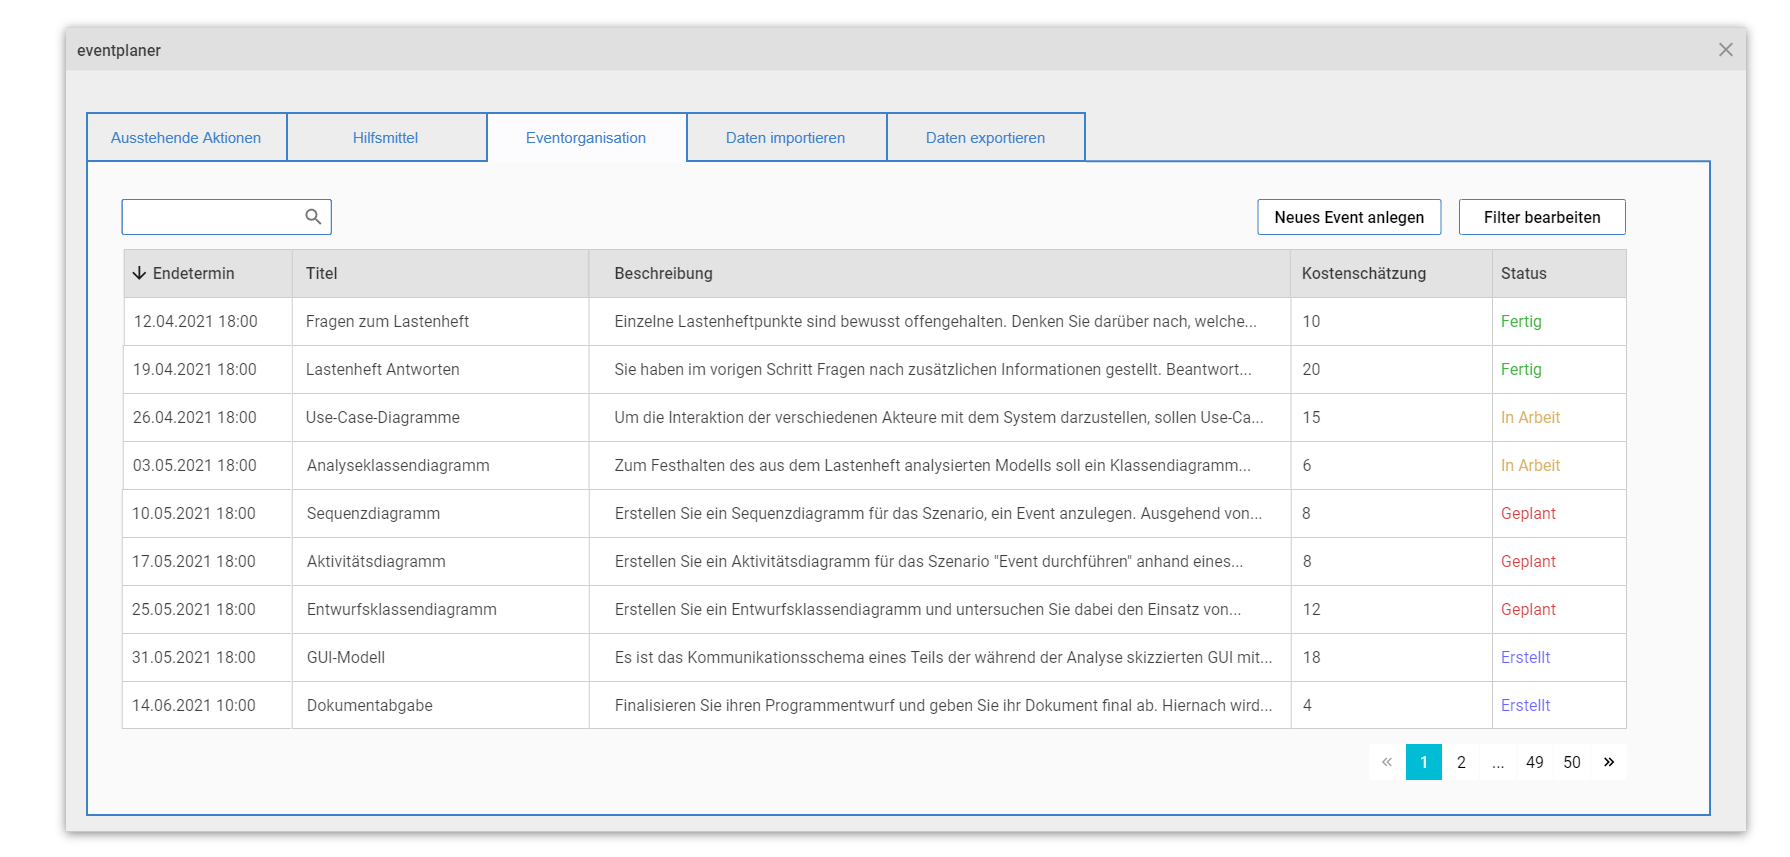
\includegraphics[width=0.98\columnwidth]{Bilder/mockup_eventorganisation.png}
    \caption{Übersicht der Events}
    \label{gui:übersicht-events}
\end{figure}
\newpage
\FloatBarrier
\subsection{Template auswählen}
Möchte ein Organisator ein neues Event anlegen, so hat er die Möglichkeit, dieses auf Basis eines Eventelements, also eines Templates, zu tun. Darum wird ihm beim Anlegen eines Events zunächst das in \autoref{gui:template-auswählen} modellierte GUI angezeigt, sodass er entweder eines der vorgefertigten Templates auswählen oder, falls er mit einem leeren Event starten möchte, \enquote{Blank} auswählen kann.

\begin{figure}[ht!]
    \centering
    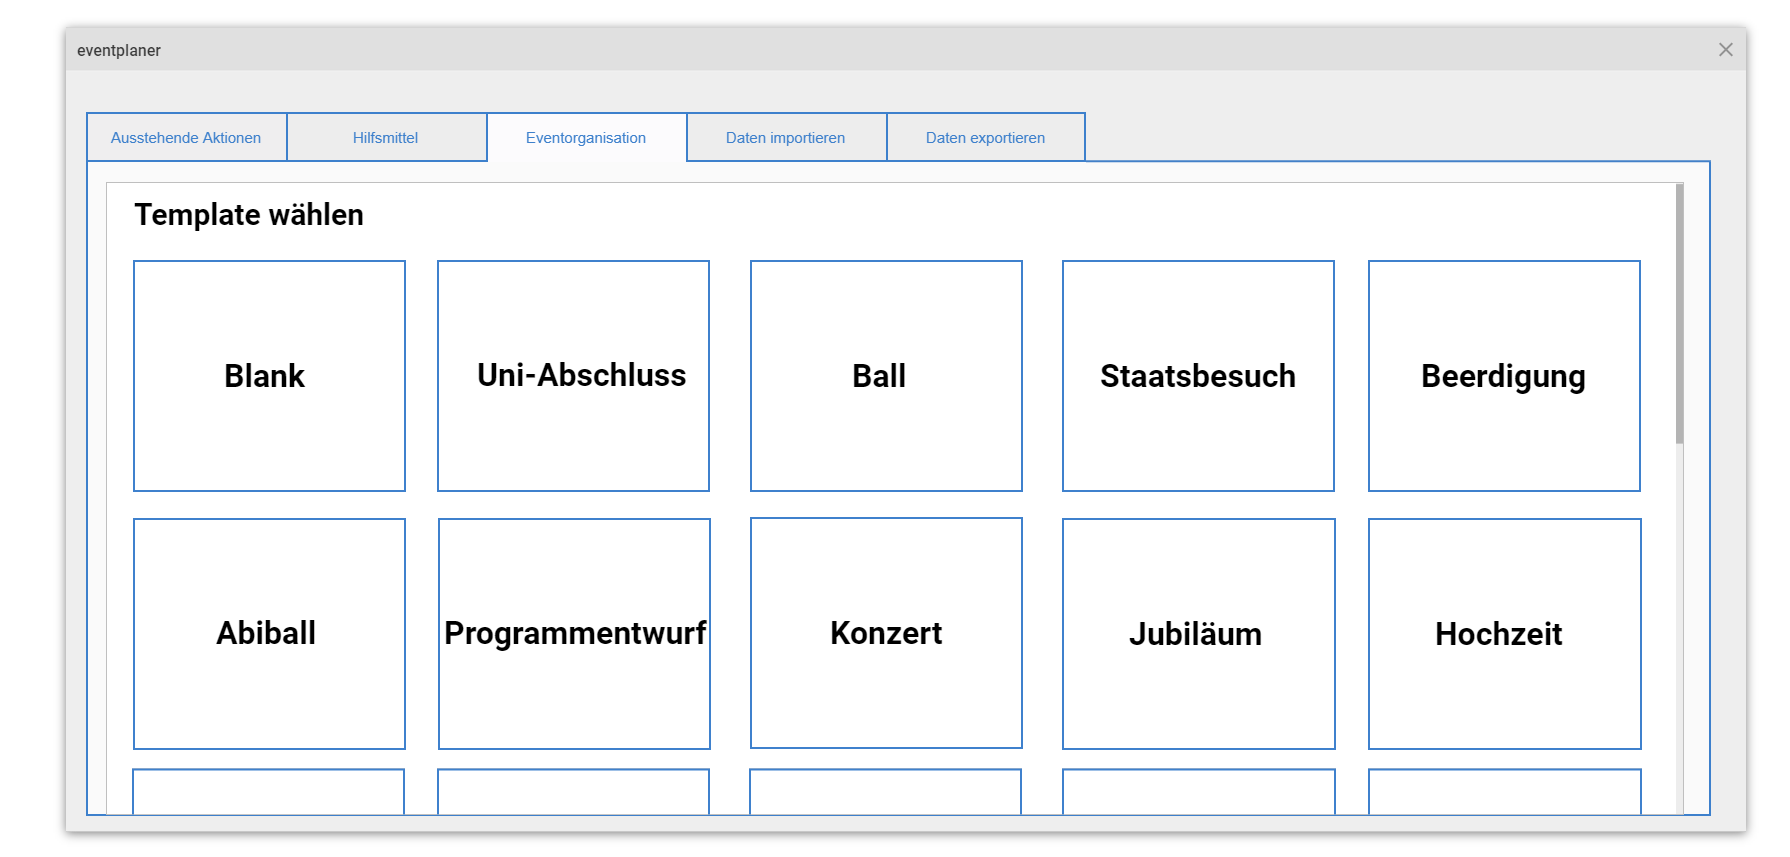
\includegraphics[width=0.98\columnwidth]{Bilder/mockup_neues_event_anlegen_templateauswahl.png}
    \caption{Template auswählen}
    \label{gui:template-auswählen}
\end{figure}

\newpage
\subsection{Neues Event anlegen und Attribute setzen}
Hat sich der Organisator für ein Template bzw. das leere Event entschieden, wird ihm der in \autoref{gui:event-anlegen} gezeigte Screen angezeigt. Hier kann der Organisator die primitiven Attribute Titel, Beschreibung und Kategorie des Events setzen, außerdem werden Start- und Endetermin sowie der Verantwortliche für das Event ausgewählt. Auf der rechten Seite hat der Organisator die Möglichkeit, dem Event in verschiedenen Tabs Verweise, Bilder und untergeordnete Teileinheiten hinzuzufügen.

\begin{figure}[ht!]
    \centering
    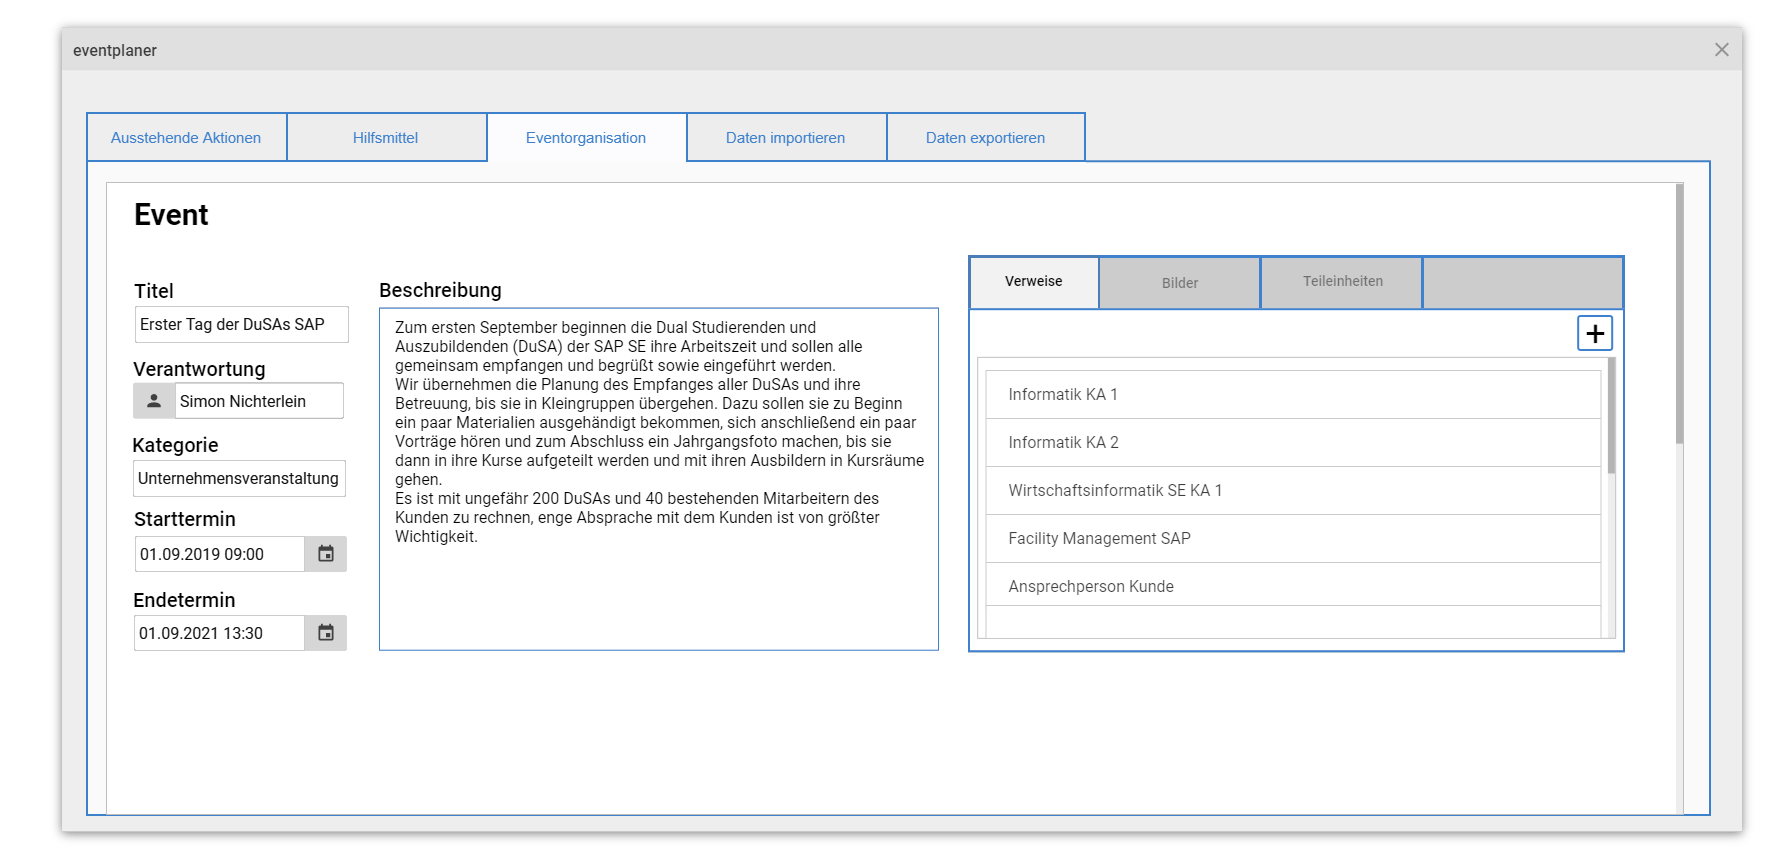
\includegraphics[width=0.98\columnwidth]{Bilder/mockup_neues_event_anlegen_attribute_setzen.png}
    \caption{Neues Event anlegen}
    \label{gui:event-anlegen}
\end{figure}

\newpage
\FloatBarrier
\subsection{Ausstehende Aktionen eines Mitarbeiters}
In der in \autoref{gui:ausstehende-teilevents} gezeigten Ansicht werden jedem Mitarbeiter individuell die ihm zugeordneten Aktionen angezeigt, welche noch nicht abgeschlossen wurden. Um ein einheitliches Look and Feel zu erreichen, werden auch die Aktionen tabellarisch mit den Attributen Endetermin, Titel, Beschreibung, Kostenschätzung und Status angezeigt. Diese können wie die Events im vorherigen Abschnitt ebenfalls gefiltert und durchsucht werden. Auch hier werden diese seitenweise geladen, außerdem sind die Events nach Endetermin sortiert, sodass diejenigen Event ganz oben stehen, welche als nächstes abgeschlossen werden müssen.

\begin{figure}[ht!]
    \centering
    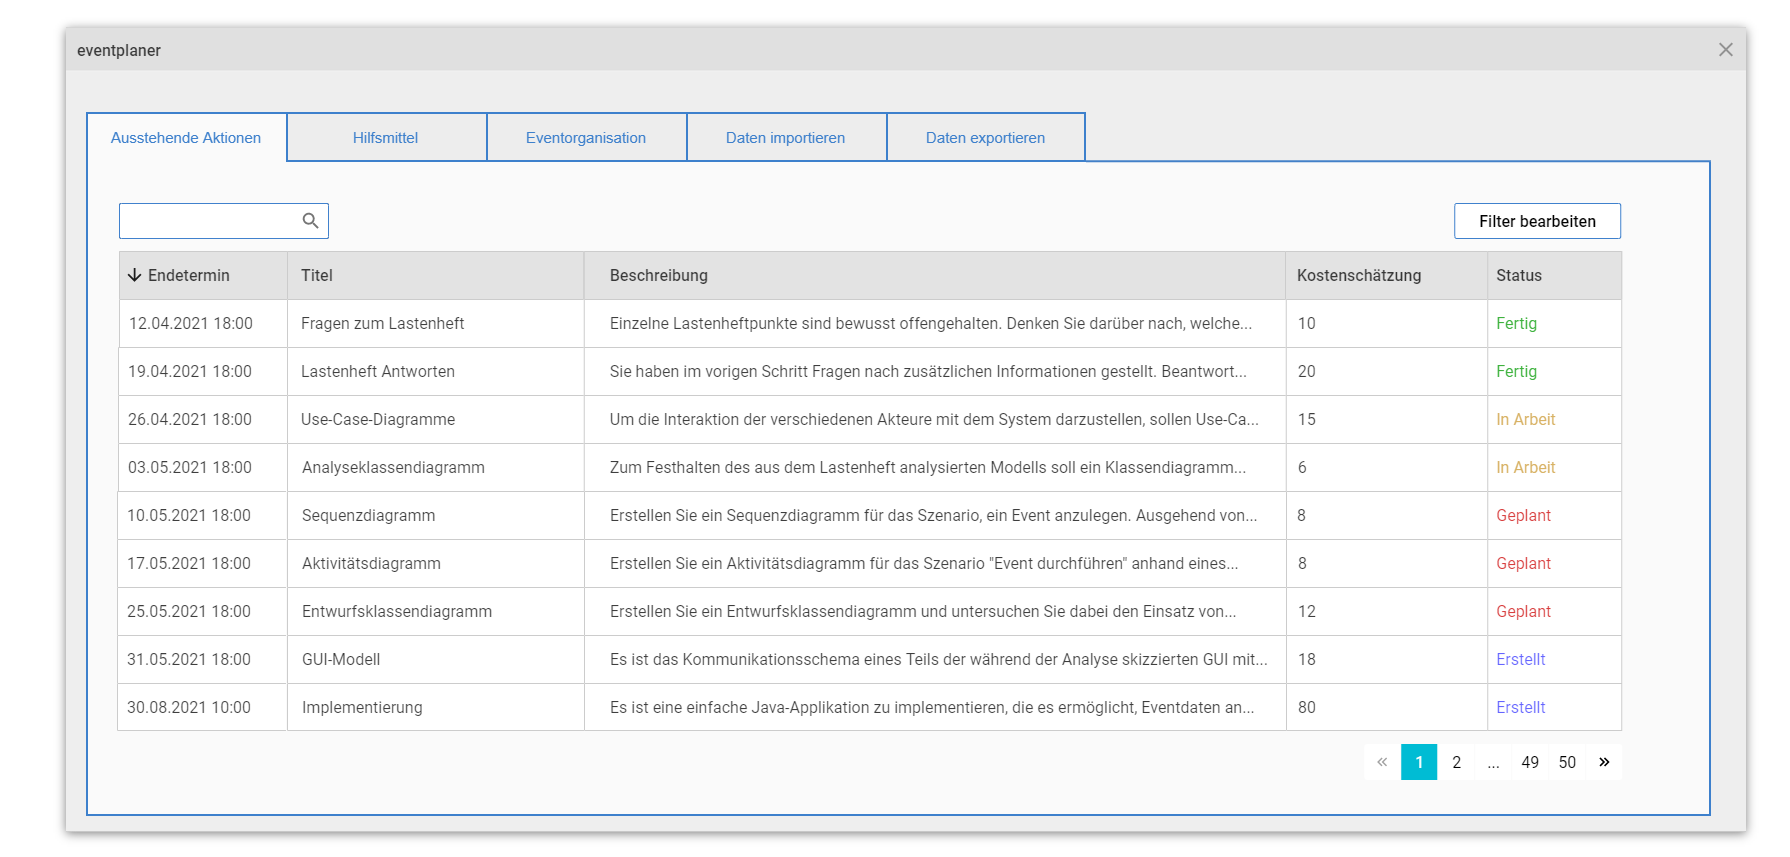
\includegraphics[width=0.98\columnwidth]{Bilder/mockup_ausstehende_teilevents.png}
    \caption{Ausstehende Aktionen eines Mitarbeiters}
    \label{gui:ausstehende-teilevents}
\end{figure}

\newpage
\FloatBarrier
\subsection{Übersicht der Hilfsmittel}
\autoref{gui:übersicht-hilfsmittel} zeigt die Hauptansicht der Hilfsmittelverwaltung, auf der die im System hinterlegten Hilfsmittel tabellarisch angezeigt werden. Zu sehen sind in der Übersicht die Attribute Materialnummer, Name, Lagerort, Menge sowie die Klasse des Hilfsmittels, also ob es sich um ein Gebrauchs- oder Verbrauchsgut handelt. Auch die Hilfsmittel werden seitenweise geladen und können durchsucht und gefiltert werden. Ferner kann mit Hilfe des Buttons \enquote{Gebrauchsgut anlegen} oder \enquote{Verbrauchsgut anlegen} ein neues Hilfsmittel angelegt werden.

\begin{figure}[ht!]
    \centering
    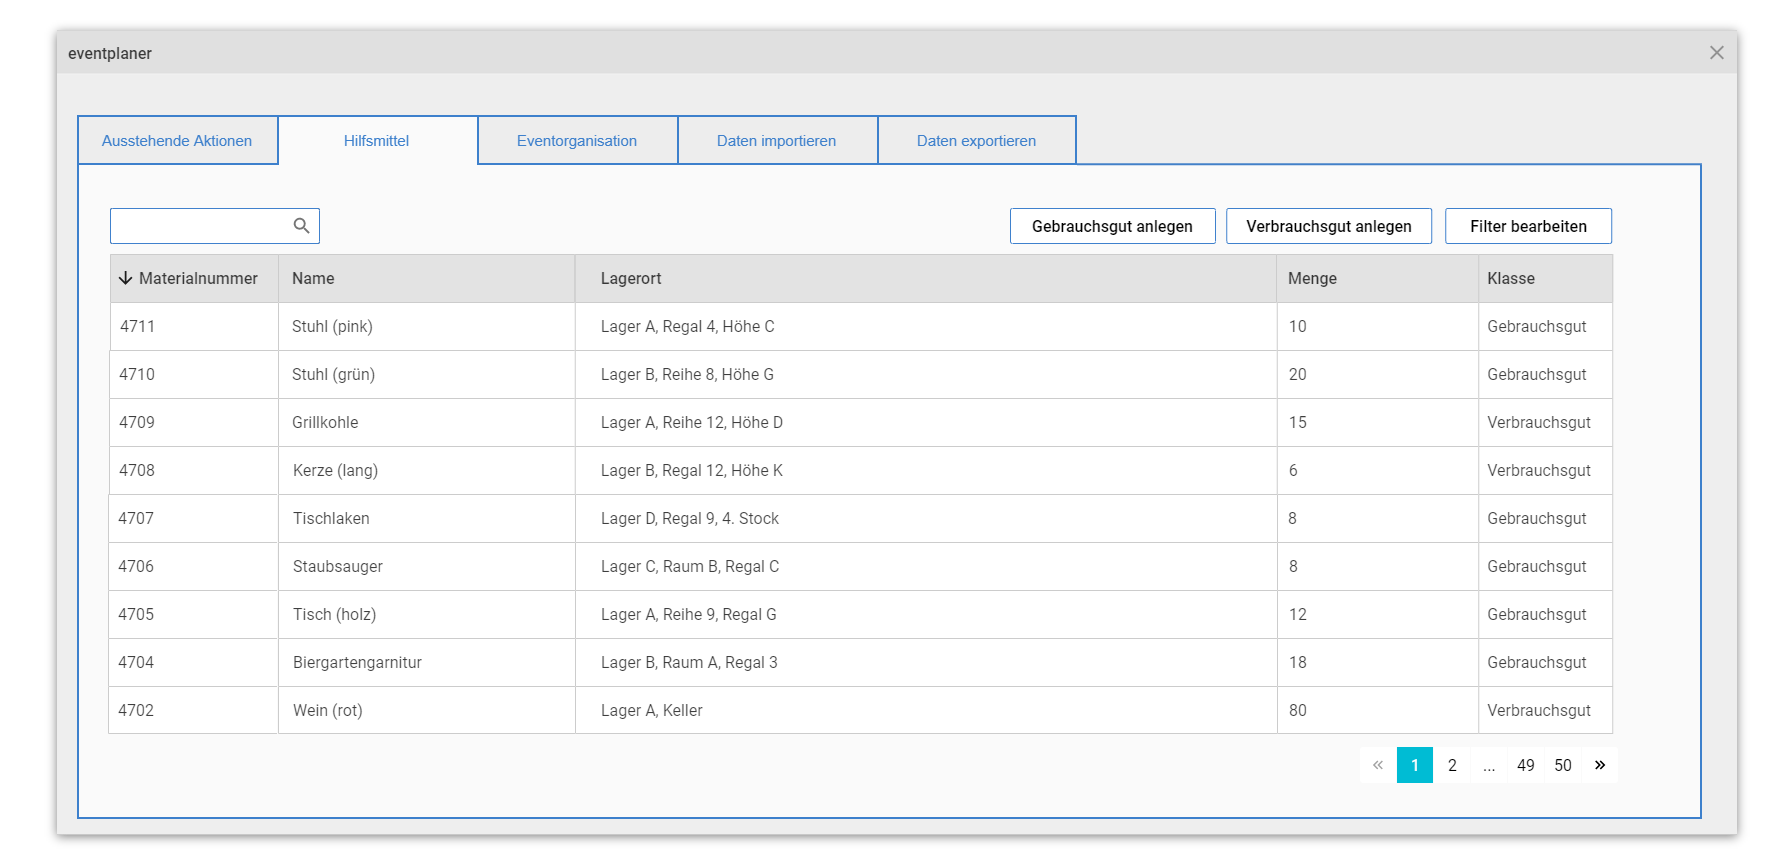
\includegraphics[width=0.98\columnwidth]{Bilder/mockup_hilfsmittel.png}
    \caption{Übersicht der Hilfsmittel}
    \label{gui:übersicht-hilfsmittel}
\end{figure}

\newpage
\FloatBarrier
\subsection{Datenimport}
Das UI für den Import von Events wurde in \autoref{gui:datenimport} modelliert. Hier kann der Nutzer mittels des Buttons \enquote{Datei auswählen} zunächst die CSV-Datei mit den für den Import vorgesehenen Daten auswählen. Diese werden anschließend geladen und in der Tabelle angezeigt, jedoch noch nicht importiert. Als nächstes hat der Nutzer die Möglichkeit, die Events zu filtern. Erfüllt ein Event nicht die Filterkriterien, so wird die entsprechende Checkbox in der Spalte \enquote{Ausgewählt?} ausgegraut und dahinter das Wort \enquote{Filter} angezeigt. Bei den restlichen Events kann der Nutzer mit Hilfe der Checkbox individuell entscheiden, ob er diese importieren möchte oder nicht. Standardmäßig sind alle nicht ausgefilterten Events ausgewählt.

\begin{figure}[ht!]
    \centering
    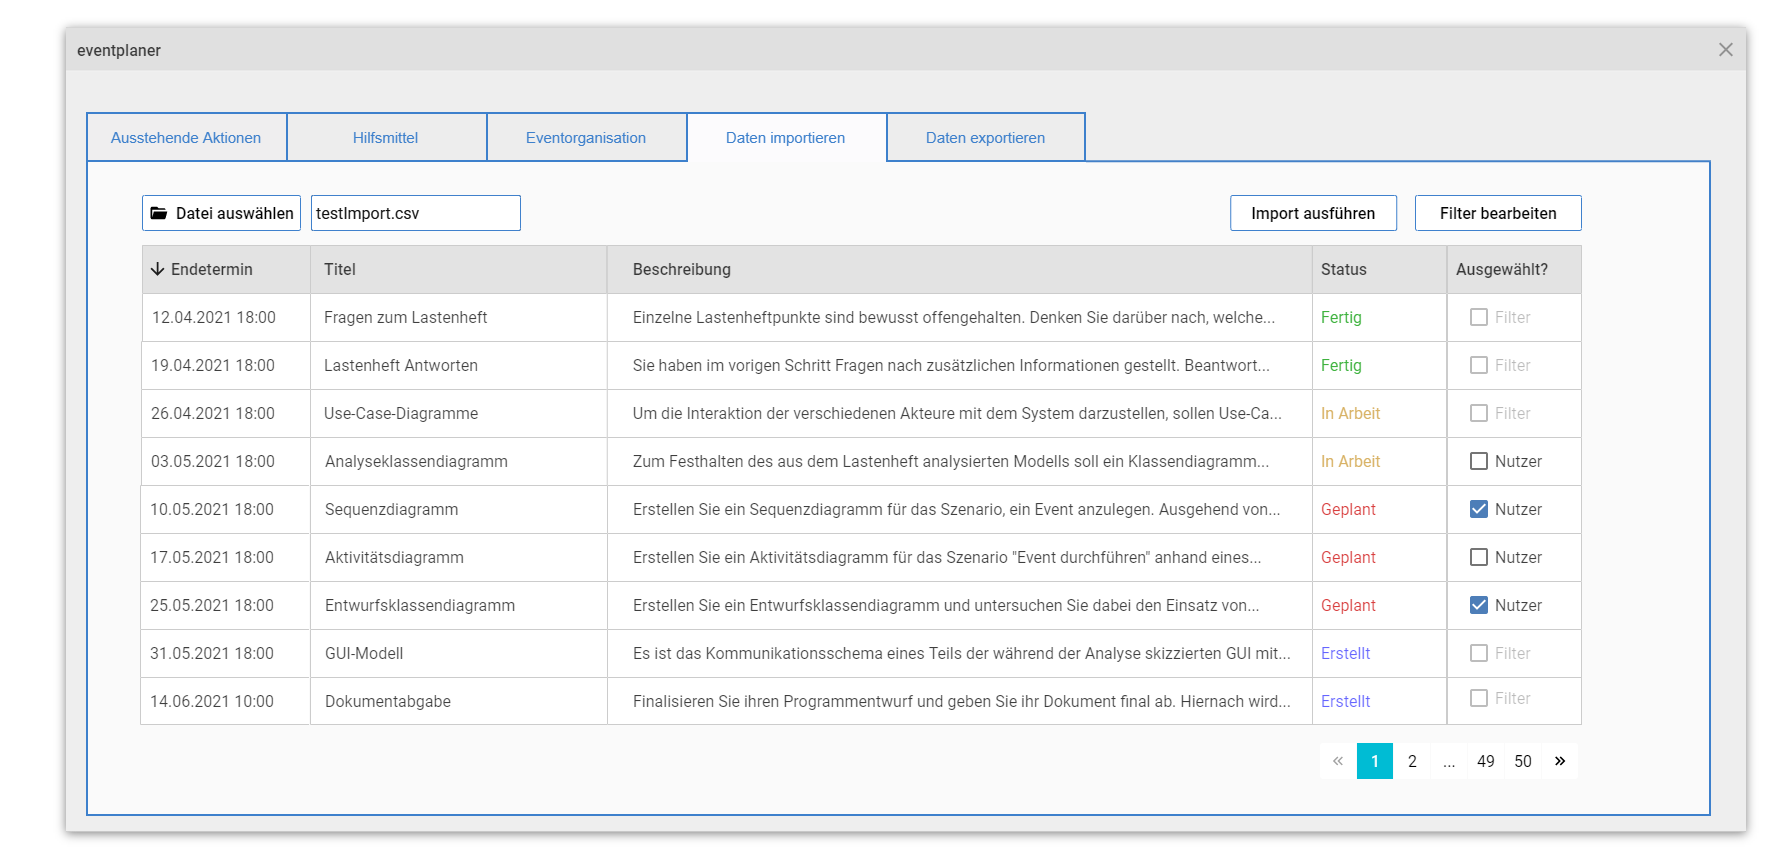
\includegraphics[width=0.98\columnwidth]{Bilder/mockup_daten_importieren.png}
    \caption{Datenimport}
    \label{gui:datenimport}
\end{figure}

\newpage
\FloatBarrier
\subsection{Datenimport mit Filtern}
Klickt der Nutzer während des Imports auf den Button \enquote{Filter bearbeiten}, so ändert sich die Anzeige wie in \autoref{gui:datenimport-filter} gezeigt: Rechts wird weiterhin die Tabelle mit den zu importierenden Events angezeigt, allerdings in kompakterer Form, links können die Filter bearbeitet werden. Dort wird jeder Filter durch eine Zeile repräsentiert. In der linken Zelle steht jeweils das Attribut, nach dem gefiltert werden soll, in der mittleren der logische Vergleichsoperator und ganz rechts der Wert, mit dem verglichen werden soll. Mit dem Button \enquote{Neuer Filter} kann eine weitere Zeile und damit ein weiterer Filter hinzugefügt werden und mit dem Button \enquote{Filter anwenden} wird das Bearbeiten der Filter beendet und diese angewendet.

\begin{figure}[ht!]
    \centering
    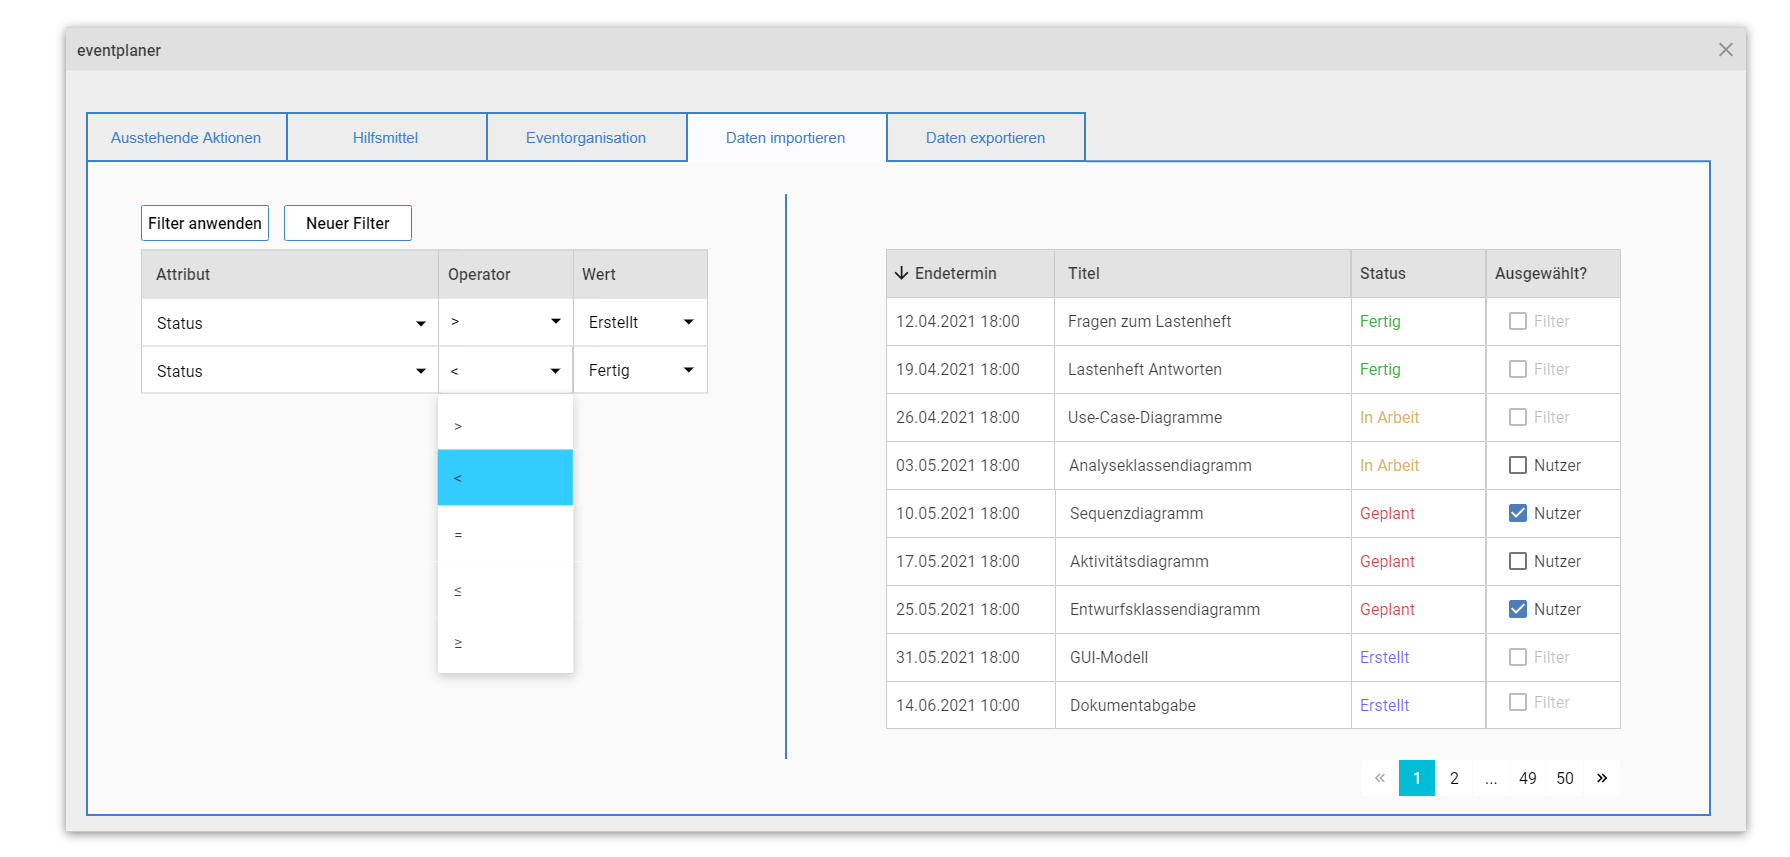
\includegraphics[width=0.98\columnwidth]{Bilder/mockup_daten_importieren_filter.png}
    \caption{Datenimport mit Filtern}
    \label{gui:datenimport-filter}
\end{figure}

\chapter{Use-Case-Diagramme}
\begin{figure}[ht!]
    \centering
    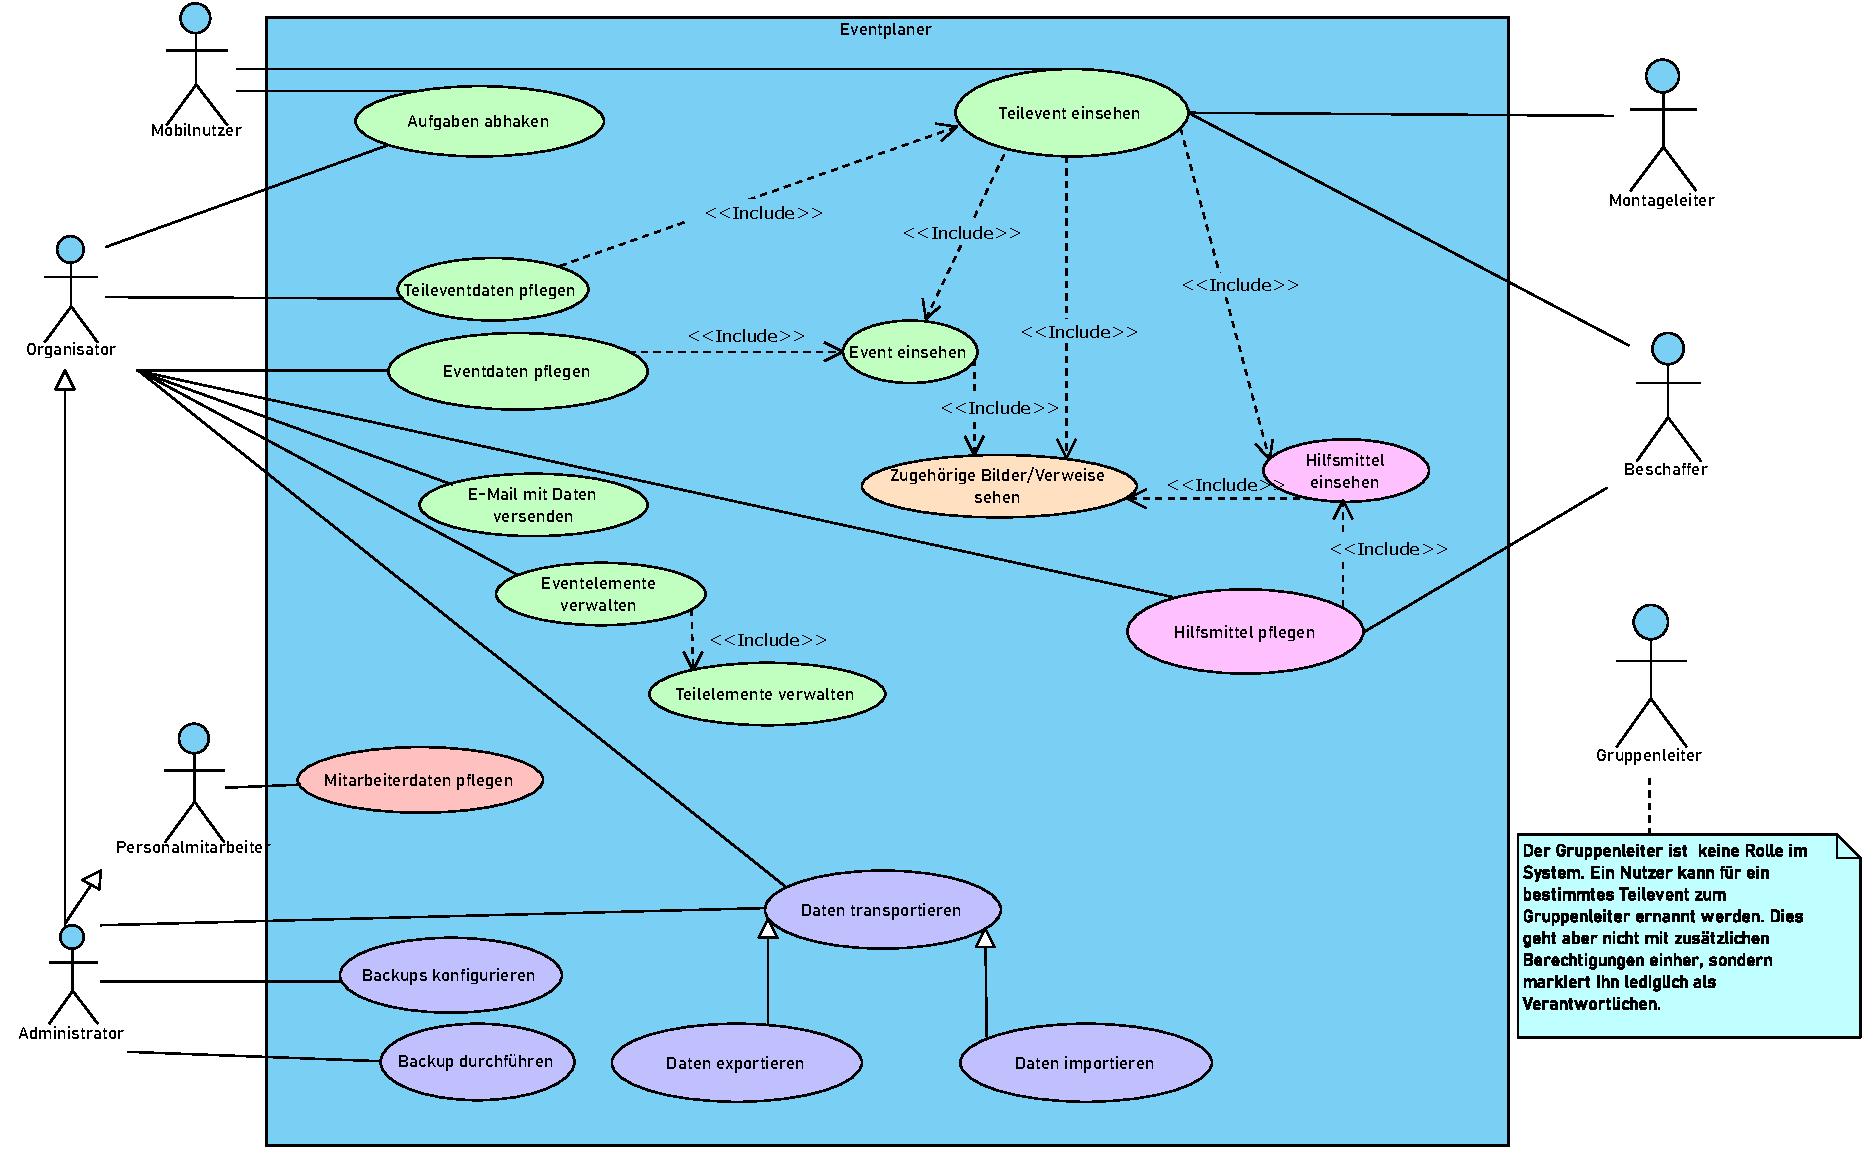
\includegraphics[width=0.98\columnwidth]{Bilder/use-case-diagramm-grob.pdf}
    \caption{Use-Case-Diagramm der gesamten Anwendung}
    \label{fig:uc:grob}
\end{figure}
Abbildung ~\ref{fig:uc:grob} zeigt die Use-Cases der gesamten Anwendung. Verschiedene Farben kennzeichnen die verschiedenen Themengebiete. Zuerst werden alle Use-Cases grob dargestellt und beschrieben sowie deren Zusammenhänge gezeigt.

\section{Erläuterung der Akteure}
Der Eventplaner besitzt fünf Rollen, die Nutzern zugewiesen werden können. Der Gruppenleiter und Mobilnutzer sind keine dem Nutzer zuweisbare Rollen. Durch die zugewiesene Rolle wird festgelegt, welche Zugriffsrechte ein Nutzer im System hat. Im Folgenden soll jeder in den Diagrammen auftauchende Akteur kurz erläutert werden. Es wird immer nur die männliche Formulierung der Rolle für alle Geschlechter verwendet.

\paragraph{Montageleiter}
Der Montageleiter hat lesenden Zugriff auf seinen Arbeitsbereich betreffende Objekte. Aus der Analyse ergibt sich, dass dieses die ihm zugewiesenen Teilevents sowie alle darüberstehenden Teilevents und Events sind. Damit kann der Montageleiter auch die dem Teilevent zugewiesenen Hilfsmittel, Bilder und Verweise betrachten. 

Zu beachten ist, dass der Montageleiter, auch wenn er für das Teilevent verantwortlich ist, es nicht als abgeschlossen markieren kann. Aus der Analyse ergibt sich, dass das durch einen Anruf an den Organisator geschieht, welcher es dann im System einträgt. Des Weiteren kann der Montageleiter keine Veränderungen an der Verantwortlichkeit des Teilevents tätigen. Ist dieser zum Beispiel auch der Gruppenleiter des Projektes und meldet sich eine weitere freiwillige Person, die helfen möchte, muss auch hier der Organisator diese eintragen.

\paragraph{Beschaffer}
Das Beschaffungspersonal besorgt und verwaltet Hilfsmittel. Dafür hat es Zugriff auf die zugewiesenen Teilevents, die übergeordneten Teilevents und Events, sowie zugewiesenen Hilfsmittel, Bilder und Verweise. Des Weiteren hat das Beschaffungspersonal aber auch noch Zugriff darauf, Hilfsmittel zu verwalten. 

Dadurch sollen Organisatoren davon entlastet werden, die genauen Details der Hilfsmittel zu verwalten. Trotzdem müssen auch Beschaffer dem Organisator manuell mitteilen, dass eine Aufgabe erledigt ist und abgehakt werden kann.

\paragraph{Administrator}
Der Administrator hat Zugriff auf jegliche Funktionalität. Er ist der einzige Akteur, der ein Backup ausführen kann und die automatischen wöchtenlichen Backups konfigurieren kann.

\paragraph{Personalmitarbeiter}
Der Personalmitarbeiter nutzt das System nur, um die Mitarbeiterdaten zu verwalten. Er benötigt keine Funktionalität, die mit dem Kerngeschäft der Eventplanung zu tun hat, da sein Aufgabenbereich nicht das Kerngeschäft beinhaltet.

\paragraph{Organisator}
Der Organisator hat als Leiter und Planer von Events die meisten Rechte. Er kann Events planen und somit auch alle Daten dazu, sowie zu untergeordneten Teilevents einsehen. Er kann diese Daten jedoch nicht nur einsehen, sondern auch in jeder Weise bearbeiten. Des Weiteren können Organisatoren E-Mails mit Informationen an Personen senden, die es betrifft sowie ausführliche Daten-Exporte und -Importe durchführen.

Eine wichtige Aufgabe des Organisators ist es, während der Durchführung eines Events die einzelnen Teilevents abzuhaken, sobald Mitarbeiter mitteilen mit einer Aufgabe fertig zu sein.

\paragraph{Mobilnutzer}
Der Mobilnutzer ist in diesem Konzept eine Person vor Ort, die entweder Informationen zu dem ihr zugewiesenen Teilevent einsehen möchte oder eines der zugewiesenen Teilevents abhaken möchte. Der Mobilnutzer kann somit ihm zugewiesene Teilevents einsehen, sowie die zugehörigen Daten. Auch kann dieser ihm direkt zugewiesene Teilevents als fertig markieren. Das ermöglicht es, ein Teilevent abzuschließen, ohne dass der Organisator involviert wird.

Der Mobilnutzer ist somit keine Rolle, die einem durch den Personalmitarbeiter zugewiesen wird, sondern man implizit ausübt, wenn durch die Mobilversion auf das System zugegriffen wird.

\paragraph{Gruppenleiter}
Der Gruppenleiter ist keine Rolle im System, die von einem Personalmitarbeiter einem Nutzer zugewiesen wird. Ein Mitarbeiter kann für ein bestimmtes Teilevent zum Gruppenleiter ernannt werden. Dieses gibt ihm keine weiteren Berechtigungen, aber markiert ihn als Verantwortlichen für dieses Teilevent.

\section{Erläuterung der Use-Cases}

\paragraph{Zugehörige Bilder sehen}
Ein wesentliches Feature der Software ist die Möglichkeit, verschiedensten Elementen wie Events oder Hilfsmitteln Bilder zuzuordnen. Diese im Nachhinein dann einsehen zu können, ist darum ein integraler Use-Case für den Eventplaner, welcher darum auch in einigen anderen Use-Cases verwendet wird.

\paragraph{Hilfsmittel einsehen}
Zur Planung und Durchführung von Events ist eine Vielzahl sogenannter Hilfsmittel notwendig. Dies können beispielsweise Kerzen bei einer Hochzeit oder Stühle und Tische für einen Kongress sein. Als Teil vieler anderer Use-Cases müssen diese eingesehen beziehungsweise gefiltert und durchsucht werden können.

\paragraph{Hilfsmittel pflegen}
Dieser Use-Case betrifft die Verwaltung der Hilfsmittel unabhängig von bestimmten Events. Er umfasst beispielsweise Funktionalitäten wie das Hinzufügen und entfernen von Hilfsmitteln aus der Datenbasis oder das pflegen der Lagerbestände. Dieser Use-Case ist nur Benutzern mit den Rollen \enquote{Beschaffer} oder \enquote{Organisator} zugänglich.

\paragraph{Teilevent einsehen}
Dieser Use-Case dient dem Einsehen der Daten eines Teilevents. Er setzt sich aus mehreren weiteren Use-Cases zusammen: Da der Nutzer das gewünschte Teilevent auch im Kontext des Übergeordneten Events betrachten können soll, beinhaltet dieser Use-Case auch das \enquote{Event einsehen}. Da einem Teilevent auch Bilder zugeordnet werden können, ist auch der Use-Case \enquote{Zugehörige Bilder sehen} Teil dieses Use-Cases. Ein weiterer wichtiger Bestandteil sind die Hilfsmittel eines Teilevents.

\paragraph{Teileventdaten pflegen}
Jedes Teilevent besitzt eine Vielzahl von Attributen. Diese können sowohl primitiv wie Name und Beschreibung als auch Assoziationen zu anderen Elementen wie beispielweise den Hilfsmitteln oder untergeordneten Teilevents sein. Diese müssen durch die Organisatoren bearbeitet werden können. Handelt es sich um Assoziationen, so soll die Auswahl möglichst mittels Auswahllisten erfolgen. Selbstverständlich umfasst dieser Use-Case auch das \enquote{Teilevent einsehen}.

\paragraph{Event einsehen}
Zur Verrichtung ihrer Tätigkeiten müssen Nutzer die Möglichkeit haben, die Daten der Events einzusehen. Dieses umfasst neben primitiven Attributen und Assoziationen auch das Einsehen der zugehörigen Bilder.

\paragraph{Eventdaten pflegen}
Analog zu den Attributen eines Teilevents müssen auch die Attribute der übergeordneten Events bearbeitet werden können. Dieses umfasst auch das \enquote{Event einsehen}. Auch dieser Use-Case ist lediglich den Organisatoren zugänglich.

\paragraph{E-Mail mit Daten versenden}
Zur besseren Kommunikation mit anderen Beteiligten haben Organisatoren die Möglichkeit E-Mails mit Daten eines Events oder Teilevents zu versenden. Diese werden durch die Software automatisch generiert und dann im Standardmailclient des verwendeten Endgeräts sendebreit geöffnet.

\paragraph{Mitarbeiterdaten pflegen}
Um die Mitarbeiter adäquat zu bestimmten Teilevents zuordnen zu können müssen bestimmte Informationen über die Mitarbeiter in der Software erfasst und ggf. geändert werden können. Diese Aufgabe und somit auch dieser Use-Case obliegt allein den Personalmitarbeitern.

\paragraph{Daten exportieren}
Die in der Software verwalteten Daten können in Form von CSV-Dateien exportiert werden. Hierbei hat der Nutzer die Möglichkeit, die zu exportierenden Daten nach den Attributen der gewünschten Objekte zu filtern.

\paragraph{Daten importierten}
Analog zum Expotieren von Daten ist auch ein Import von Daten aus CSV-Dateien möglich und auch hier hat der Nutzer die Möglichkeit, bevor er den Import ausführt die zu importierenden Daten nach deren Attributen zu filtern.

\paragraph{Daten transportieren}
Dieser Use-Case fasst die beinden ihm untergeordneten Use-Cases \enquote{Daten exportieren} und \enquote{Daten importieren} zusammen. Er ist, außer natürlich dem Administrator, lediglich den Organisatoren zugänglich.

\paragraph{Backups konfigurieren}
Der Administrator hat die Möglichkeit durch das System automatisch durchzuführende Backups zu konfigurieren. Dieser Use-Case umfasst das Festlegen des Zielverzeichnisses, in welchem die gesicherten Daten gespeichert werden sollen, sowie den Zeitpunkt, zu dem das Backup ausgeführt werden soll.

\paragraph{Backups durchführen}
Neben den automatischen Backups bietet das System auch die Möglichkeit, Backups manuell durchzuführen. Allerdings steht auch dieser Use-Case nur dem Administrator zur Verfügung.

\paragraph{Aufgaben abhaken}
Das Abhaken von Aufgaben ist ein Use-Case, welcher erst in der zweiten Ausbaustufe der Software von Interesse sein wird. Hier muss es dem Nutzer möglich sein, erledigte Aufgaben mittels einer Mobile-App abzuhaken, also als abgeschlossen zu markieren.

\section{Verfeinerung des Use-Case \enquote{Teileventdaten pflegen}}
\begin{figure}[ht!]
    \centering
    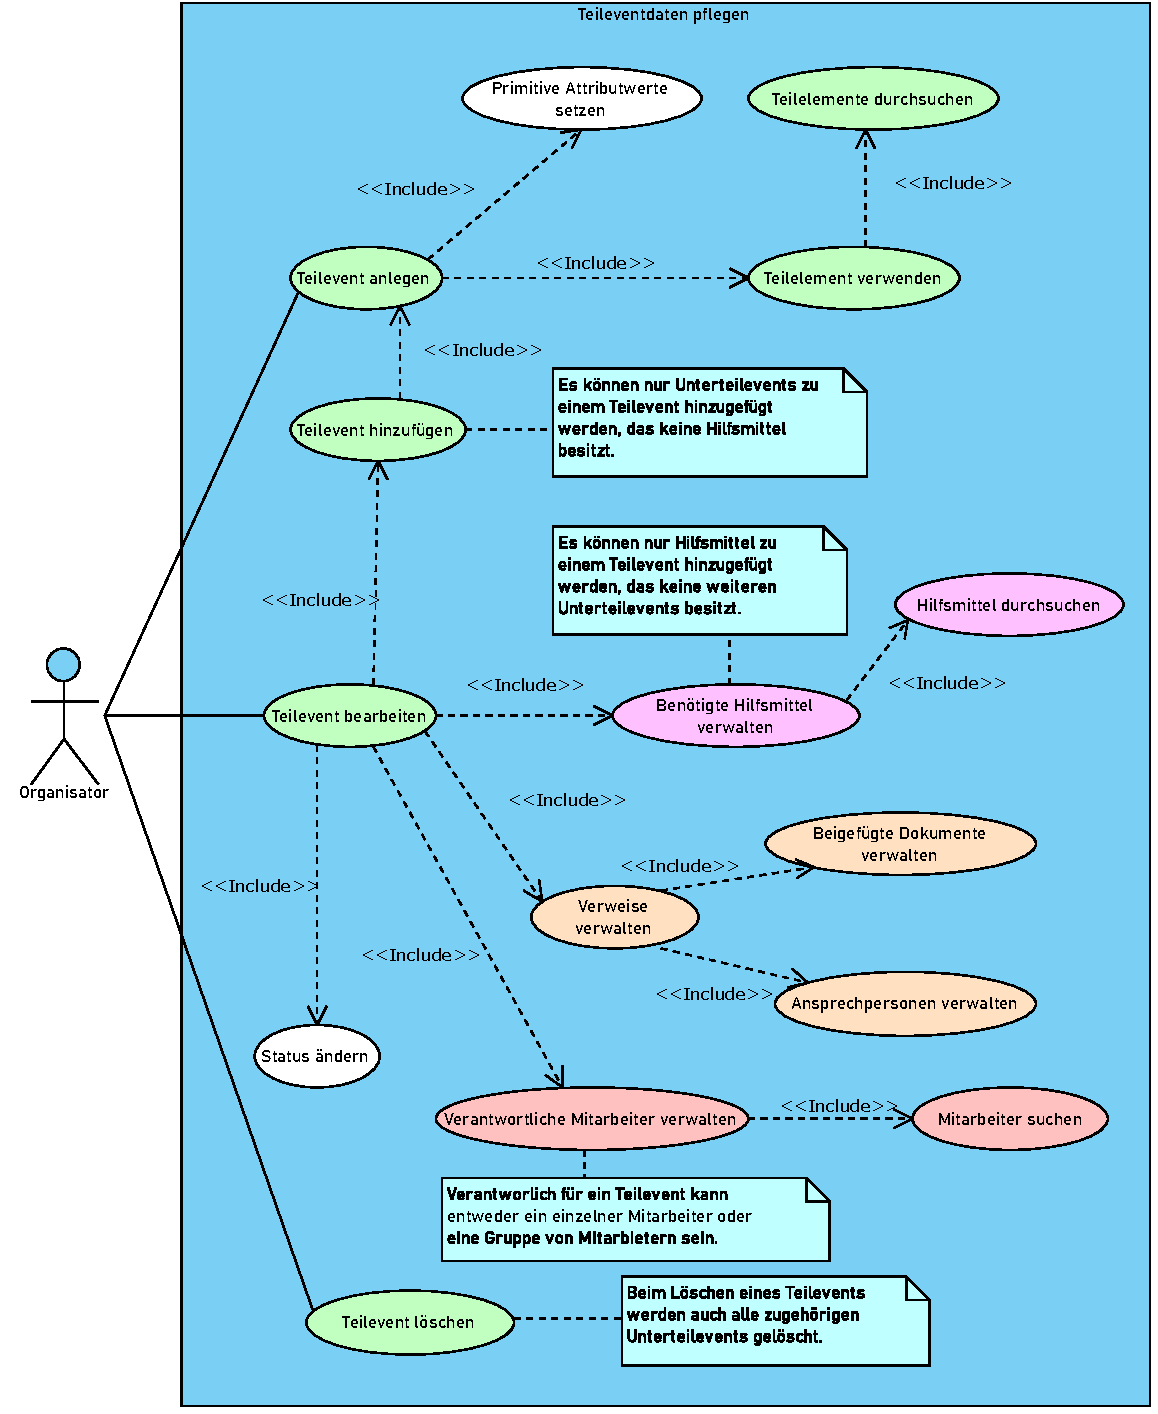
\includegraphics[width=0.98\columnwidth]{Bilder/use-case-diagramm-fein.pdf}
    \caption{Use-Case-Diagramm des Use-Case \enquote{Teileventdaten pflegen}}
    \label{fig:uc:fein}
\end{figure}

\paragraph{Teilelemente durchsuchen}
Die vorhandenen Teilelemente können durch Freitext durchsucht werden. Der Suchtext wird mit den Attributen des Teilelements verglichen und bei Übereinstimmung in der Ergebnisliste angezeigt. Dieses dient dazu, den Nutzer dabei zu unterstützen schnell die korrekten Teilelemente zu finden, um diese auswählen zu können.

\paragraph{Teilelement verwenden}
Es kann ein vorgefertigtes Teilelement als Vorlage für ein neues Teilevent verwendet werden. Dadurch kann die bereits bei anderen Events getane Arbeit wiederverwendet werden. Trotzdem müssen dann noch die primitiven Attribute vervollständigt werden.

\paragraph{Primitive Attribute setzen}
Beim Anlegen müssen die primitiven Attribute eines Teilevents gesetzt werden. Dazu gehören unter Anderem der Name, die Start- und Endtermine und die Beschreibung. Dadurch hat jedes Teilevent direkt nach dem Anlegen schon grundlegende Informationen und kann so weiterverwendet werden.

\paragraph{Teilevent anlegen}
Es können neue Teilevents angelegt werden. Dafür kann entweder ein Teilelement als Vorlage verwendet werden oder blank begonnen werden. Beim Anlegen werden die primitiven Attribute gesetzt und sobald dieses geschehen ist, kann angefangen werden, die weiteren Attribute und zugehörigen Objekte zu verwalten.

\paragraph{Teilevent hinzufügen}
Zu einem bestehenden Teilevent können Unterteilevents hinzugefügt werden. Dieses Teilevent stellt dann keine konkrete Aktion dar, die durchgeführt werden soll, sondern eine logische Gruppierung von Teilevents, die wiederum Gruppen an Aktionen sein könnten. Wird ein Unterteilevent hinzugefügt, so können diesem Teilevent keine Hilfsmittel hinzugefügt werden. Um ein Unterteilevent hinzuzufügen, muss dieses Unterteilevent dafür grundsätzlich neu angelegt werden.

\paragraph{Hilfsmittel durchsuchen}
Hilfsmittel können anhand einer Freitextsuche gefiltert werden. Der Suchtext wird dann mit den Attributen verglichen und bei Übereinstimmung wird das Hilfsmittel in der Ergebnisliste angezeigt. Dieses dient der Benutzerfreundlichkeit, da das Eventplanungsunternehmen eine große Basis an Hilfsmitteln hat, die nicht manuell komplett durchsucht werden soll.

\paragraph{Benötigte Hilfsmittel verwalten}
Ein Teilevent, welches keine Unterteilevents hat, stellt eine Aktion dar, die ausgeführt werden soll. Daher können diesem Teilevent Hilfsmittel zugeordnet werden, die zur Durchführung benötigt werden oder diese unterstützen. Hilfsmittel die einem Teilevent zugeordnet sind, sind für den Zeitraum des Teilevents gebucht. Die Zuordnung eines Hilfsmittel geschieht durch eine Suche mit anschließender Auswahl.

\paragraph{Beigefügte Dokumente verwalten}
Einem Verweis können beliebige Dokumente zugeordnet werden. Diese werden in dem Verzeichnis der zentralen Datenbasis abgelegt. In diesem Use-Case können diese Dokumente angelegt oder gelöscht werden. Ein Beispiel dafür wäre der Mietvertrag der Location eines Events, dadurch kann auch dieser im System verwaltet werden und geht nicht verloren.

\paragraph{Ansprechpersonen verwalten}
Einem Verweis können beliebig viele Ansprechpersonen zugeordnet werden, diese halten jeweils die Kontaktdaten dieser Person für zukünftige Zwecke fest. Ein Beispiel für eine Ansprechperson wäre der Hausmeister der Halle, die für ein Konzert verwendet wird. In diesem Use-Case können dann neue Ansprechpersonen angelegt, vorhandene bearbeitet oder gelöscht werden.

\paragraph{Verweise verwalten}
Zu jedem Teilevent können beliebig viele Verweise angelegt werden. In dem Verweis ist optional ein Firmenname eingetragen und dem Verweis können Dokumente und Ansprechpersonen zugeordnet werden.

\paragraph{Mitarbeiter suchen}
Mitarbeiter können in einer Freitextsuche gefunden werden. Der Freitext wird mit allen Attributen des Mitarbeiters verglichen und zutreffende Mitarbeiter in einer Ergebnisliste angezeigt. Dieses wird hier dafür verwendet, die Mitarbeiter für die Zuweisung der Verantwortlichkeit auszusuchen.

\paragraph{Verantwortliche Mitarbeiter verwalten}
Die Verantwortlichkeit für ein Teilevent kann bei der Bearbeitung festgelegt werden. Wird beim Erstellen keine Verantwortlichkeit festgelegt, so ist der Ersteller standardmäßig verantwortlich. Es kann ein einzelner Mitarbeiter oder eine Gruppe an Mitarbeitern als verantwortlich markiert werden. Wird eine Gruppe als verantwortlich markiert, muss einer der Mitarbeiter als Gruppenleiter markiert werden. Die Mitarbeiter werden durch eine Suche ausgewählt.

\paragraph{Status ändern}
Der Status eines Teilevents kann geändert werden. Dabei wird aus einer Auswahlliste einer der möglichen vordefinierten Status ausgewählt. Dieses ist eine Veränderung eines primitiven Attributes. Durch diese Funktionalität kann der Organisator zum Beispiel Aufgaben abhaken, sobald sie ihm als erledigt gemeldet werden oder als \enquote{geplant} markieren, um eine Übersicht darüber zu haben, was er bereits fertig geplant hat.

\paragraph{Teilevent bearbeiten}
Ein Teilevent kann nach der Erstellung immer noch bearbeitet werden. Dabei können alle primitiven Attribute verändert und zugehörige Objekte verwaltet werden. Dieses ermöglicht es, das Teilevent nachträglich noch zu ändern, falls sich die Umstände ändern oder bei der Planung Fehler geschehen sind.

\paragraph{Teilevent löschen}
Sollte ein Teilevent als unnötig angesehen werden, soll natürlich die Möglichkeit bestehen, dieses zu löschen. Wird es gelöscht, so müssen kaskadierend auch alle Unterteilevents des Teilevents gelöscht werden, da ein Teilevent nicht ohne Ober(teil)event existieren kann.


\chapter{Analyseklassendiagramm}
In Abbildung ~\ref{fig:akd} sind alle im Lastenheft erkannten Entitäten erfasst und es stellt die Beziehungen zwischen diesen umfassend dar. Diese Darstellungen sind durch die Analyse der Anwendungsfälle der Eventplanungssoftware sowie die Analyse des Lastenheftes entstanden.

\begin{figure}[ht!]
    \centering
    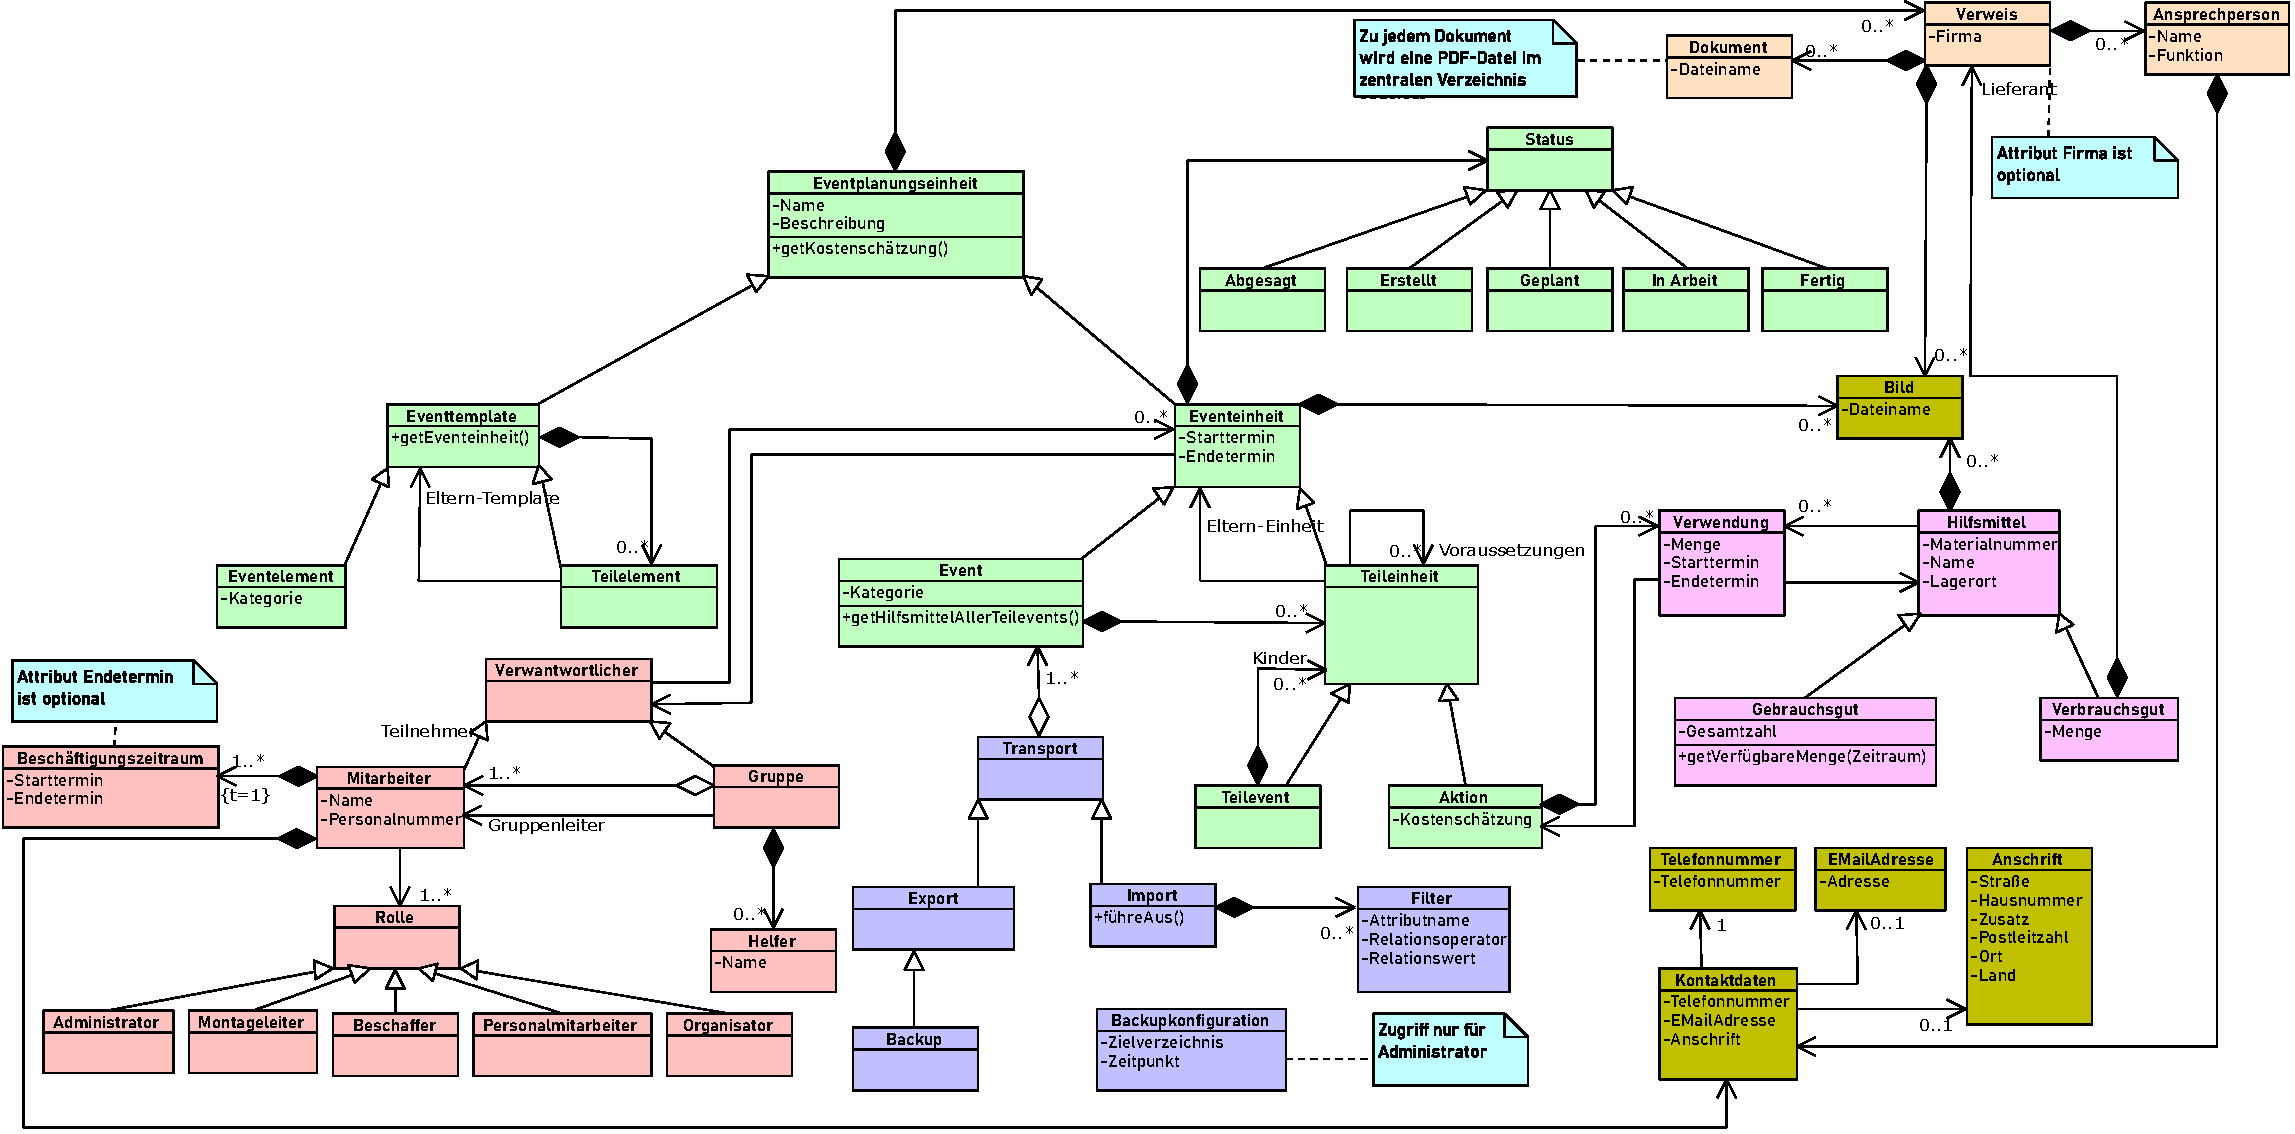
\includegraphics[width=0.98\columnwidth]{Bilder/akd.pdf}
    \caption{Analyseklassendiagramm mit Ansicht aller Objekte in der Eventplanung}
    \label{fig:akd}
\end{figure}

Zur Übersichtlichkeit wurden die Entitäten je nach Bereich eingefärbt. Alle dem Personal und der Verantwortlichkeit für eine Eventeinheit zuzuordnenden Entitäten sind rot eingefärbt, alle für Hilfsmittel wichtigen Klassen sind pink, alle das Transportsystem betreffenden Klassen sind violett. Die Klassen, welche die Struktur des Eventablaufes und dessen Planung betrachten sind grün eingefärbt, während Verweise und dazugehörendes orange sind. Alle Hilfsklassen, die zwischen zwei Bereichen stehen, sind grünbraun eingefärbt. Im Folgenden werden zuerst die einzelnen Entitäten erläutert und anschließend wird näher auf die verwendeten Analysemuster eingegangen.

\section{Analyse der verschiedenen Objekte}

\paragraph{Transport}
Ein Transportobjekt ist eine Aggregation von Events. Ein Transportobjekt sollte nie instantiiert werden, sondern nur die Unterklassen. Es beschreibt eine Menge an Events, die importiert, exportiert oder zur Datensicherung gespeichert werden sollen.
\paragraph{Export}
Exporte beschreiben eine Menge an Events im System, die exportiert werden sollen. Der Export findet zur Datensicherung im Falle eines Backups statt und sonst zur Weitergabe bestimmter Eventdaten. Die Events für den Export werden anhand von Filtern ausgewählt und dann in dem Exportobjekt gesammelt.
\paragraph{Import}
Ein Importobjekt ist eine aus einer Datei gelesene Ansammlung von Events, die dafür bestimmt sind, in das System hinzugefügt zu werden. Auf diesen Import können Filter angewendet werden, bevor dieser mit \code{führeAus()} die dann noch durch die Filter ausgewählten Events im System einpflegt.
\paragraph{Filter}
Ein Filterobjekt wird dafür verwendet, eine Teilmenge von Events aus einer Obermenge auszuwählen. Dafür werden jeweils der Name des Attributs gespeichert, mit dem verglichen werden soll, der Vergleichsoperator, der dafür verwendet werden soll und der Wert, mit dem verglichen werden soll. Damit können jegliche simple Filter realisiert werden, wie zum Beispiel, dass der Starttermin später als 2020 ist. Diese Filter können beispielsweise bei Export- und Import-Aktionen verwendet werden.
\paragraph{Backup}
Ein Backup ist eine spezielle Form des Exports, bei dem alle Events zur Datensicherung auf einem externen Medium gespeichert werden. Backups können automatisch wöchentlich durch die Backupkonfiguration festgelegt stattfinden oder manuell von einem Administrator ausgeführt werden.
\paragraph{Backupkonfiguration}
Die Backupkonfiguration legt zentral fest, wann wöchentliche Backups stattzufinden haben und in welchem Zielverzeichnis diese abgelegt werden sollen. Die Backupkonfiguration kann von einem Administrator verändert werden.

\paragraph{Verweis}
Ein Verweisobjekt ist eine zentrale Zusammenfassung aller Daten zu einem externen Objekt, häufig einer Firma. Er enthält ein einziges Attribut zum Festhalten des Firmennamens, welches optional ist, damit auch nicht-Firmen-Verweise dargestellt werden können. Ein Verweis enthält eine Sammlung an Dokumenten, Bildern und Ansprechpersonen. Diese Objekte sind jeweils nur vorhanden, solange auch der Verweis existiert. Sie werden also gelöscht, wenn der Verweis gelöscht wird. Ein Verweis muss kein weiteres Objekt enthalten, sondern kann auch vollkommen leer initialisiert werden. Der Hauptnutzen eines Verweises ist es, externe Dokumente und Objekte im System abzubilden, damit sie vom Nutzer eingesehen werden können.
\paragraph{Dokument}
Das Dokumentobjekt beschreibt ein von einem Nutzer zu einem Verweis hinzugefügtes Dokument, welches er für zukünftige Zwecke festhalten möchte. Dabei wird als Attribut der Dateiname gespeichert, den die Datei im zentralen Verzeichnis hat, auf dem Dokumente und Bilder abgelegt werden. Dokumente können nur einem Verweis hinzugefügt werden, jedoch nicht einem Event direkt. Beispielhaft für ein Dokument wäre ein Mietvertrag, der einem Verweis auf die verwendete Halle einer Hochzeit zugeordnet wird.
\paragraph{Ansprechperson}
Das Ansprechpersonobjekt beschreibt eine Kontaktperson zu einem Verweis. Dieses ist zum Beispiel der Hausmeister einer Halle oder der Verkäufer bei einem Lieferanten. Dafür werden der volle Name sowie die Funktionsbezeichnung dieser Kontaktperson gespeichert. Der Name wird als einzelnes Attribut gespeichert, damit jegliche Kombination von Name, Vorname und Mittelnamen vollständig und ohne Probleme abgebildet werden kann, ohne dass jede Besonderheit einzeln im Modell beachtet werden muss. Zu der Kontaktperson werden auch noch Kontaktdaten gespeichert, damit gesichert ist, dass diese immer kontaktiert werden kann.

\paragraph{Verantwortlicher}
Eine Eventeinheit benötigt immer exakt einen Verantwortlichen, der die Verantwortung dafür trägt, dass diese Eventeinheit erfolgreich und vollständig abgeschlossen wird. Diese Verantwortung kann von einer Einzelperson oder einer Gruppe mit Gruppenleiter getragen werden. Damit ist immer eine Einzelperson identifizierbar, die dafür verantwortlich ist, aber auch abgebildet, dass mehrere Personen an der Erfüllung der Aufgabe beteiligt sein können.
\paragraph{Gruppe}
Ein Gruppenobjekt beschreibt, dass eine Menge an Menschen an dem Teilevent oder Event arbeitet. Jede Gruppe hat exakt einen Gruppenleiter, der gleichzeitig auch ein Teilnehmer der Gruppe ist, daher hat jede Gruppe mindestens einen Teilnehmer. Die Teilnehmer einer Gruppe sind Mitarbeiter des Unternehmens. Des Weiteren kann eine Gruppe noch Helfer beinhalten, die auch an der Eventeinheit beteiligt sind.
\paragraph{Helfer}
Ein Helferobjekt stellt einen Helfer dar, der nicht bei dem Unternehmen angestellt ist. Zu diesen Helfern wird nur der Name gespeichert. Dadurch ist es möglich, schnell und einfach externe Hilfskräfte im System festzuhalten. Da sich externe Hilfskräfte in der Vergangenheit als äußerst unzuverlässig erwiesen haben, wird sich in der Planung nicht auf deren Anwesenheit verlassen. Externe Hilfskräfte sind zum Beispiel die Mutter der Braut, die gerne dabei helfen möchte, die Stühle aufzubauen. Dafür wird sie im System als Helfer eingetragen, sodass der verantwortliche Gruppenleiter darüber Bescheid weiß.
\paragraph{Mitarbeiter}
Über jeden Mitarbeiter werden im System Daten zu Name, Personalnummer, den Berechtigungen, Kontaktdaten und Beschäftigungszeiträumen gespeichert. Es müssen nicht viele Daten über diesen gespeichert werden, da der Großteil bereits im Personalbuchhaltungssystem verwaltet wird und für die Eventplanung nicht notwendig ist. Jeder Mitarbeiter kann befristet oder unbefristet eingestellt sein. Zur Zeit nicht eingestellte Mitarbeiter werden weiter im System behalten, um so zum Beispiel Saisonarbeiter verwalten zu können, die immer wieder ein befristetes Verhältnis mit dem Unternehmen eingehen.
\paragraph{Beschäftigungszeitraum}
Im Beschäftigungszeitraumobjekt werden jeweils der Starttermin und der Endetermin eines Beschäftigungsverhältnisses zwischen einem Mitarbeiter und dem Unternehmen festgehalten. Dieses ist wichtig, um planen zu können, ob befristete Mitarbeiter bei einem zukünftigen Event noch zur Verfügung stehen oder bereits nicht mehr eingestellt sind. Dadurch sind auch Saisonarbeiter gut unterstützt, die nur während der Hochsaison für Events eingestellt werden.
\paragraph{Rolle}
Die Rollen eines Mitarbeiters beschreiben seine Berechtigungen im System. Jeder Mitarbeiter hat mindestens eine Rolle und kann jede Rolle höchstens einmal haben. 
\begin{itemize}
    \item \textbf{Administrator} - Die Administratorrolle gibt dem Mitarbeiter die Berechtigung alles zu tun, was eine andere Rolle kann und noch die Backups zu konfigurieren und auszuführen. Diese Rolle ist nur zum Aufsetzen und für administrative Zwecke im System erforderlich.
    \item \textbf{Montageleiter} - Der Montageleiter hat das Recht, ihm zugewiesene Teilevents im Kontext zu sehen, um die ihm damit zugewiesenen Aufgaben erledigen zu können.
    \item \textbf{Beschaffer} - Der Beschaffer hat das Recht, ihm zugewiesene Teilevents im Kontext zu sehen, um die ihm damit zugewiesenen Aufgaben erledigen zu können. Des Weiteren kann dieser Hilfsmittel verwalten.
    \item \textbf{Personalmitarbeiter} - Personalmitarbeiter sind für die Verwaltung des Personals zuständig. Sie können Mitarbeiter verwalten, ihnen Rollen zuweisen oder ihre Beschäftigung verändern. Sie sind auch dafür verantwortlich, relevante Daten aus dem Personalbuchhaltungsprogramm in dem Eventplanungssystem festzuhalten.
    \item \textbf{Organisator} - Der Organisator plant Events, daher kann er Eventplanungseinheiten verwalten. Dazu zählt es, diese anzulegen, zu bearbeiten oder auch zu löschen. Des Weiteren kann der Organisator Events importieren und exportieren.
\end{itemize}

\paragraph{Status}
Die Klasse Status bildet die Oberklasse aller Status, in welchen sich eine Eventeinheit, also ein Event oder Teilevent befinden kann. Damit besitzt der Status die folgenden Unterklassen, welche jeweils einen konkreten Status repräsentieren:
\begin{itemize}
    \item \textbf{Erstellt} - In diesem Status befindet sich eine Eventeinheit unmittelbar nach dem Anlegen und während der Planungsaktivitäten.
    \item \textbf{Geplant} - Ist die Planung einer Eventeinheit sowie ihrer untergeordneten Teilevents vollständig abgeschlossen, so befindet sich die Eventeinheit im Status \enquote{Geplant}.
    \item \textbf{In Arbeit} - Während der eigentlichen Durchführung einer Eventeinheit befindet sich diese im Status \enquote{In Arbeit}.
    \item \textbf{Fertig} - Ist eine Eventeinheit vollständig abgeschlossen, so befindet sie sich im Status \enquote{Fertig}. 
    \item \textbf{Abgesagt} - Ist eine Eventeinheit nicht mehr durchzuführen, so wird diese in den Status \enquote{Abgesagt} gesetzt.
\end{itemize}

\paragraph{Bild}
Da einer Vielzahl von Objekten auch Bilder zugeordnet werden können, bedarf es für diese auch eine programmatische Repräsentation. Dies geschieht mittels der Klasse Bild, welche jedoch als Attribut lediglich den Namen der zugehörigen Bilddatei besitzt, anhand welchem das Bild geladen werden kann, sobald notwendig.

\paragraph{Verwendung}
Die Klasse Verwendung bildet die Zuweisung von Hilfsmitteln zu Aktionen ab. Hilfsmittel werden durch eine Verwendung jeweils in einer bestimmten Menge über einen bestimmten Zeitraum gebucht. Darum besitzt die Verwendung als Attribute die Menge sowie einen Start- und einen Endetermin. Sie verweist außerdem jeweils auf das gebuchte Hilfsmittel sowie auf das Teilevent, für welches das Hilfsmittel gebucht wird.

\paragraph{Kontaktdaten}
Da sowohl zu Ansprechpersonen als auch zu Mitarbeitern Kontaktdaten gespeichert werden müssen, werden diese durch eine separate Klasse abgebildet. Diese besitzt Assoziationen zu Telefonnummer, EMailAdresse und Anschrift. Allerdings sind EMailAdresse und Anschrift optional, lediglich eine Telefonnummer ist verpflichtend.

\paragraph{Eventplanungseinheit}
Die Eventplanungseinheit ist die Oberklasse der nachfolgend beschriebenen Klassen Eventtemplate und Eventeinheit. Sie liefert die primitiven Attribute Name und Beschreibung sowie eine Getter-Methode für die Kostenschätzung der jeweiligen Einheit. Hierbei haben Instanzen der Eventplanungseinheit ohne weitere Untereinheiten (Unterteilevents oder Unterteilelemente) eine manuell einzutragende Kostenschätzung, bei allen anderen ist die Kostenschätzung die Summe der Kosten der Untereinheiten. Ferner besitzt jede Eventplanungseinheit beliebig viele Verweise.

\paragraph{Eventemplate}
Das Eventtemplate bildet wiederum die Oberklasse des Eventelements und des Teilelements, da es sich bei beiden um vorgefertigte Templates für Eventeinheiten, also Events bzw. Teileinheiten handelt. Jedes Eventtemplate besitzt beliebig viele untergeordnete Teilelemente. Es handelt sich hierbei um eine Komposition, da die Existenz der untergeordneten Teilelemente von der des Eventtemplates abhängt. Ferner besitzt das Eventtemplate die Methode \code{getEventeinheit()}, welche aus dem Template ein Eventelement bzw. ein Teilelement mit voreingestellten Attributwerten generiert.

\paragraph{Eventelement}
Bei dem Eventelement handelt es sich um ein Template für ein Event. Es besitzt außer den von den Überklasssen Eventplanungseinheit und Eventtemplate geerbten Attributen noch das Attribut Kategorie. Dieses ermöglicht es, dem Event ein Schlagwort wie \enquote{Hochzeit} oder \enquote{Kongress} zuzuordnen.

\paragraph{Teilelement}
Bei einem Teilelement handelt es sich um ein Template für eine Teileinheit. Es besitzt ebenfalls die Attribute der Oberklassen Eventplanungseinheit und Eventtemplate. Darüber hinaus besteht eine Assoziation zu seinem Eltern-Template. Hierbei kann es sich entweder um ein weiteres Teilelement oder ein Eventelement handeln.

\paragraph{Eventeinheit}
Die zweite Unterklasse der Eventplanungseinheit ist die Eventeinheit. Sie wiederum bildet die Oberklasse des Events sowie der Teileinheit und liefert die Attribute Starttermin und Endetermin. Beide Attribute beinhalten jeweils ein Datum und eine minutengenaue Uhrzeit. Ferner besitzt jede Eventeinheit stets einen Status. Bei dieser Assoziation handelt es sich um eine Komposition, da ein einzelner Status ohne zugehöriges Objekt keinen Sinn ergeben würde. Des weiteren können jeder Eventeinheit beliebig viele Bilder zugewiesen werden. Da die Bilder mit einer Eventeinheit fest verknüpft sind und nicht unabhängig von diesen existieren können, handelt es sich auch bei dieser Assoziation um eine Komposition.

\paragraph{Event}
Die Klasse Event erbt von der Oberklasse Eventeinheit. Sie erweitert diese um das Attribut \enquote{Kategorie}, welches analog zum gleichnamigen Attribut des Eventelements die Möglichkeit bietet, dem Event ein bestimmtes Schlagwort zuzuordnen. Ein Event hat beliebig viele untergeordnete Teileinheiten, welche nur gekoppelt mit dem Event existieren können. Daher ist diese Assoziation als Komposition modelliert worden. Da das Event keine eigenen Hilfsmittel besitzt, sondern lediglich die Hilfsmittel der ihm untergeordneten Teilevents kumuliert, besitzt es die Methode \code{getHilfsmittelAllerEvents()}, welche eine Liste aller den untergeordneten Teileinheiten zugewiesenen Hilfsmitteln liefert.

\paragraph{Teileinheit}
Ebenso wie das Event erbt auch die Teileinheit von der Oberklasse Eventeinheit und ist selbst Oberklasse von Teilevent und Aktion. Da jede Teileinheit einer weiteren Teileinheit oder einem Event untergeordnet ist, besitzt es eine Assoziation zu einer Eventeinheit, nämlich die ihm übergeordnete Elterneinheit. Ferner können einzelne Teileinheiten von anderen Teileinheiten abhängig sein. So müssen beispielsweise vor dem Aufbau der Tischdekoration bei einer Hochzeit erst die Tische aufgebaut werden. Um derartige Umstände abzubilden, besitzt jede Teileinheit beliebig viele Voraussetzungen, also Teileinheiten, welche zuvor abgeschlossen sein müssen.

\paragraph{Teilevent}
Das Teilevent stellt eine Menge an Teileinheiten dar, die inhaltlich zusammen gehören und somit zusammen geplant werden. Es erbt von der Teileinheit und hat beliebig viele Teileinheiten als Kinder.

\paragraph{Aktion}
Eine Aktion ist eine konkrete Tätigkeit, die durchgeführt wird und nicht weiter in kleinere Tätigkeiten zu zerteilen ist. Daher hat diese Aktion dann auch eine konkrete, manuell eingetragene Kostenschätzung und der Aktion können Hilfsmittel zugeordnet werden. Um dieses zu tun, verweist diese auf beliebig viele Verwendungen, die jeweils die Buchung eines bestimmten Hilfsmittels darstellen. Folglich werden diese beim Löschen eines Teilevents ebenfalls gelöscht, daher handelt es sich bei dieser Assoziation um eine Komposition.

\paragraph{Hilfsmittel}
Für die meisten Events werden Hilfsmittel benötigt. Dies können beispielsweise Tische und Stühle, Kerzen auf einer Hochzeit oder ein Rednerpult für einen Kongress sein. Jedes Hilfsmittel besitzt als Attribute eine eindeutige Materialnummer sowie einen Namen und einen Lagerort. Ferner verweist jedes Hilfsmittel auf beliebig viele Verwendungen, welche die Buchung eines Hilfsmittels für einen bestimmten Zeitraum in einer bestimmten Menge darstellen. Es werden allerdings zwei verschiedene Arten von Hilfsmitteln unterschieden, welche über die beiden Unterklassen Gebrauchsgut und Verbrauchsgut der Klasse Hilfsmittel unterschieden werden. 

\paragraph{Gebrauchsgut}
Die Klasse Gebrauchsgut erbt von der Klasse Hilfsmittel und repräsentiert Hilfsmittel, welche mehrmals verwendet werden und der Abnutzung unterliegen. Zu jedem Gebrauchsgut wird die vorhandene Gesamtzahl gespeichert, außerdem besitzt es die Methode \code{getVerfügbareMenge()}, welche die in einem gegebenen Zeitraum verfügbare Menge des Hilfsmittels bestimmt.

\paragraph{Verbrauchsgut}
Die Klasse Verbrauchsgut erbt ebenfalls von der Klasse Hilfsmittel und repräsentiert Hilfsmittel, welche nur einmal verwendet werden können, wie beispielsweise Kerzen. Da diese direkt nach der Buchung als verbraucht gelten, ist für die Verbrauchsgüter keine besondere Methode zur Mengenberechnung nötig, sondern es wird lediglich die derzeit verfügbare Menge gespeichert. Da diese Hilfsmittel außerdem regelmäßig nachbestellt werden müssen, verweist jedes Verbrauchsgut auf einen Lieferanten.

\section{Verwendete Analysemuster}
Es wurden verschiedene Analysemuster verwendet, um die Objekte der Analyse zu modellieren. Analysemuster sind schematische Lösungen für eine Klasse verwandter Probleme. Es wurden die nachfolgenden fünf Analysemuster im Analyseklassendiagramm verwendet.
\paragraph{Rollen}
Das Analysemuster der Rollen wurde bei der Assoziation von Gruppe auf Mitarbeiter verwendet, um den Gruppenleiter von restlichen Teilnehmern zu differenzieren. Ein Mitarbeiter, der Teilnehmer einer Gruppe ist, kann zugleich der Gruppenleiter einer anderen oder der gleichen Gruppe sein. Daher ist es sinnvoll diese Unterscheidung durch Rollen vorzunehmen.

\paragraph{Koordinator}
Bei der Verwendung wurde das Analysemuster des Koordinators angewendet, um zu speichern, in welchem Zeitraum und welcher Menge ein Hilfsmittel bei der Aktion verwendet wird. Damit beinhaltet die Verwendung Attribute, die für die Beziehung zwischen den Objekten wichtig sind, aber in keinem der Objekte richtig aufgehoben wären.

\paragraph{Historie}
Mit der Klasse Beschäftigungszeitraum wurde das Analysemuster Historie verwendet. Die einem Mitarbeiter zugeordneten Instanzen dieser Klasse bilden den zeitlichen Verlauf seines Anstellungsverhältnisses bei der Firma ab. Durch die Attribute \enquote{Starttermin} und \enquote{Endetermin} ist für jede Instanz der Zeitraum festgelegt. Zwar ist hierbei der Endetermin optional, dies ist jedoch notwendig, um unbefristete Beschäftigungsverhältnisse abzubilden. In diesem Fall ist der Endetermin implizit noch nicht eingetroffen oder geplant.   

\paragraph{Liste}
Das Analysemuster Liste wurde im vorliegenden Analyseklassendiagramm an zwei Stellen verwendet. Im folgenden werden diese genauer erläutert.
\begin{itemize}
    \item Jedes Event beinhaltet eine Liste von ihm untergeordneter Teileinheiten. Die Teileinheiten eines Events sind diesem fest zugeordnet und können nicht ohne es existieren, lassen sich aber löschen ohne dabei das gesamte Event zu löschen. Abweichend von der Norm kann das Event jedoch auch keine Teileinheit beinhalten, also leer sein.
    \item Analog zum Event beinhaltet das Eventtemplate eine Liste von ihm untergeordneten Teilelementen. Auch diese sind dem Eventtemplate fest zugeordnet und können nicht ohne sie existieren, lassen sich aber löschen ohne dabei das gesamte Eventtemplate zu löschen. Allerdings kann auch das Eventtemplate keine Teileinheit enthalten und weicht in dieser Hinsicht leicht von der Norm ab.
\end{itemize}

\paragraph{Stückliste}
Das Analysemuster der Stückliste wurde bei der Aufteilung der Teileinheit in Teilevent und Aktion als Ganzes und Teil in einer Baumstruktur verwendet. Dadurch können die Bedürfnisse des Kunden optimal abgebildet werden, da einer Aktion eine Kostenschätzung und Hilfsmittel zugeordnet werden, dem Teilevent als Menge mehrerer Teileinheiten jedoch nicht direkt. Hier ist nur ein Typ an Blättern, die Aktionen, vorhanden.
\chapter{Sequenzdiagramme}
Im Folgenden wird das Szenario \enquote{Event anlegen} ausführlich mit Pseudocode entwickelt, um eine Reihe an Sequenzdiagrammen zu erstellen, die den Sachverhalt visualisieren.

Bei der Darstellung der Sequenzdiagramme wurde auf die exakte Interaktion mit einer Datenbankschnittstelle oder CSV-Dateien verzichtet, da diese Details hier nicht von Relevanz sind. Stattdessen wird ein Datenbasisobjekt verwendet, welches abstrakt für alle Interaktionen des Datenschreibens und -lesens zuständig ist. Es wird auch angenommen, dass der Nutzer bereits eingeloggt ist und die entsprechende Benutzeroberfläche bereits geöffnet hat. Das setzen der grundlegenden Attribute von Objekten wird unter dem Begriff der \enquote{primitiven Attribute} zusammengefasst, wenn es möglich ist. Der Fokus liegt auf den Nachrichten und den Interaktionen dazwischen, weniger auf Details des Entwurfs.

\section{Szenariobetrachtung: Event anlegen}
In diesem Szenario wird von einem Organisator ein neues Event angelegt. Hierbei wird allerdings noch eine Vielzahl weiterer Objekte erzeugt, welche vom eigentlichen Eventobjekt referenziert werden. Hierzu zählen beispielsweise Bilder, Verweise oder Teileinheiten, welche ihrerseits wieder auf weitere Objekte verweisen können.

Das Szenario setzt sich aus mehreren Teilschritten zusammen: Zunächst muss ein initiales Eventobjekt erzeugt werden. Hierbei hat der Organisator die Möglichkeit, entweder mit einem leeren Eventobjekt zu starten oder aber ein Eventelement als Template für die Erstellung des Events zu verwenden. In diesem Fall würde das Event bereits mit einer Beschreibung, einer Kategorie und eventuell vordefinierten Teileinheiten sowie den zugehörigen Kostenschätzungen initialisiert. 

Im nächsten Schritt hat der Organisator die Möglichkeit, das Event mit Leben zu füllen, indem er ihm nach belieben Bilder, Verweise - beispielsweise auf beteiligte Firmen - sowie untergeordnete Teileinheiten zuweist und diese unter Umständen auch erstellt. Ferner weist er dem gesamten Event einen Start- und einen Endetermin sowie einen Verantwortlichen zu. Bei dem Verantwortlichen kann es sich sowohl um eine Einzelperson als auch eine Gruppe von Personen handeln.

Abschließend besteht für den Organisator noch die Möglichkeit, Änderungen an den primitiven Attributen des Events, also beispielsweise Name, Beschreibung oder Kategorie, vorzunehmen. Ist der Organisator mit dem Event zufrieden, kann es anschließend gesichert und damit seine Arbeit persistiert werden.

Aus Gründen der Übersichtlichkeit wurden die meisten der oben genannten Operationen, nämlich das Anlegen von Bildern, Verweisen und Teileinheiten sowie das Finden eines Verantwortlichen im Pseudo-Code in separate Funktionen ausgelagert und darum auch als separate Sequenzdiagramme modelliert, welche dann im Hauptdiagramm des Szenarios durch Interaktionsreferenzen aufgerufen werden. 

\section{Pseudo-Code}
Um Übersichtlichkeit und klare Struktur zu ermöglichen, wurde der Pseudocode in kleinere Unterprogramme geteilt, die aufgerufen werden. Dieses ermöglicht es ebenfalls, Abläufe nicht redundant darzustellen.

Der Kunde ist Auftraggeber und hat Wissen über die gewünschten Details des Events. Der Organisator ist Nutzer des Systems und plant die konkreten Details des Events.

\lstinputlisting[style=Pseudocode, firstline=3, lastline=43, caption={Szenario Event anlegen}]{Quellcode/sequence_diagram_pseudo.txt}

Deutlich zu erkennen sind die vielen Aufrufe zu Unterprogrammmen für das Anlegen und Hinzufügen der verschiedenen Objekte, die das Event ausmachen.

\lstinputlisting[style=Pseudocode, firstline=45, lastline=98, caption={Szenario Teileinheit anlegen}]{Quellcode/sequence_diagram_pseudo.txt}

Hier ist deutlich die Ähnlichkeit zu \code{EVENT-ANLEGEN} zu sehen. Besonders ist jedoch der rekursive Aufruf auf sich selbst, der es ermöglicht, einen Baum an Teileinheiten aufzubauen. Auch zu beachten ist, dass einer Teileinheit entweder Hilfsmittel oder Teileinheiten hinzugefügt werden können. Es ist nicht möglich, beides hinzuzufügen.

\lstinputlisting[style=Pseudocode, firstline=100, lastline=122, caption={Szenario Verantwortlichen finden}]{Quellcode/sequence_diagram_pseudo.txt}

Als Verantwortlicher kann eine Gruppe oder eine Einzelperson gewählt werden, dadurch sind die zwei verschiedenen Ausführungspfade vorhanden.

\lstinputlisting[style=Pseudocode, firstline=124, lastline=135, caption={Szenario Mitarbeiter finden}]{Quellcode/sequence_diagram_pseudo.txt}

Beim Finden eines Mitarbeiters für die Verantwortlichkeit werden nur die zu der Zeit verfügbaren Mitarbeiter angezeigt. Solange der Organisator die Suchkriterien dabei ändert, wird die Liste immer wieder aktualisiert. Wenn der Organisator sich für einen Mitarbeiter aus der Liste entscheiden sollte, wird dieser zurückgegeben. Stattdessen gibt es noch die Möglichkeit, dass der Organisator einen neuen Mitarbeiter anlegen möchte, da dieser bisher nicht im System erfasst ist. Dann wird das Unterprogramm \code{MITARBEITER-ANLEGEN} aufgerufen.

\lstinputlisting[style=Pseudocode, firstline=137, lastline=162, caption={Szenario Verweis anlegen}]{Quellcode/sequence_diagram_pseudo.txt}

Beim Anlegen eines Verweises sind alle Attribute optional. Dieses ist deutlich dadurch zu sehen, dass das Hinzufügen immer an die Bedingung geknüpft ist, dass dieses vom Nutzer gewünscht ist.

\lstinputlisting[style=Pseudocode, firstline=164, lastline=172, caption={Szenario Bild anlegen}]{Quellcode/sequence_diagram_pseudo.txt}

Hier ist deutlich zu sehen, dass in einem Bildobjekt keine Bilddaten gespeichert werden. Stattdessen ist in dem Objekt bloß der Dateiname der entsprechenden Datei im zentralen Verzeichnis hinterlegt. Auch interessant ist, dass zum Verhindern von Namensdopplungen in einer Schleife ein einzigartiger Name gesucht wird.

\lstinputlisting[style=Pseudocode, firstline=174, lastline=189, caption={Szenario Ansprechperson anlegen}]{Quellcode/sequence_diagram_pseudo.txt}

Beim Anlegen einer Ansprechperson handelt es sich um einen recht einfachen Vorgang ohne besondere Logik, da ein Ansprechpersonenobjekt nur aus seinen primitiven Attributen sowie den Kontaktdaten besteht, welche in einem separaten Unterprogramm festgelegt werden.

\lstinputlisting[style=Pseudocode, firstline=191, lastline=214, caption={Szenario Verwendung anlegen}]{Quellcode/sequence_diagram_pseudo.txt}

Um ein Hilfsmittel für eine Teileinheit zu buchen, wird das Koordinatorobjekt \enquote{Verwendung} erstellt. Diese Verwendung speichert Informationen über die Relation zwischen Teileinheit und Hilfsmittel.

\lstinputlisting[style=Pseudocode, firstline=216, lastline=239, caption={Szenario Hilfsmittel anlegen}]{Quellcode/sequence_diagram_pseudo.txt}

Beim Anlegen eines Hilfsmittels ist die Unterscheidung zwischen Gebrauchs- und Verbrauchsgut zu beachten. Zum einen muss der Organisator bei einem Gebrauchsgut die vorhandene Gesamtzahl angeben, während bei einem Verbrauchsgut die aktuell verfügbare Menge einzutragen ist. Ferner wird bei der Erstellung eines Verbrauchsgutes auch ein Verweis angelegt, da zu jedem Verbrauchsgut ein Verweis auf den Lieferanten des jeweiligen Hilfsmittels gehört.

\lstinputlisting[style=Pseudocode, firstline=241, lastline=274, caption={Szenario Mitarbeiter anlegen}]{Quellcode/sequence_diagram_pseudo.txt}

Wie man sieht, werden beim Anlegen eines Mitarbeiters nicht nur die primitiven Attribute des Mitarbeiters und dessen Kontaktdaten gepflegt, sondern auch die ihm zugewiesenen Rollen vergeben. Das Hinzufügen weiterer Rollen ist natürlich nur möglich, solange der Mitarbeiter noch nicht alle im System verfügbaren Rollen besitzt. Anschließend werden dem Mitarbeiter ein oder mehrere Beschäftigungszeiträume zugewiesen. Auch bei diesen wird stets überprüft, ob Start- und Endetermin plausibel sind.

\section{Diagramme}

In den Diagrammen werden Interaktionsreferenzen verwendet, um sich auf Unterdiagramme mit Verfeinerungen zu beziehen. In den verfeinerten Diagrammen taucht das Objekt \enquote{Observer} auf, welches jeweils den aufrufenden View darstellen soll. Es wurde sich für diese Umsetzung in den Diagrammen entschieden, da das gleiche Diagramm von verschiedenen Diagrammen aus referenziert werden kann. Ein Beispiel dafür ist das Diagramm \enquote{Teileinheit anlegen}, welches von \enquote{Teileinheit anlegen} und \enquote{Event anlegen} referenziert wird. Je nachdem, wird die angelegte Teileinheit der \enquote{TeileinheitGUI} oder \enquote{EventGUI} zurückgegeben, aber im Diagramm wird dafür einfach der \enquote{Observer} als abstrakte Darstellung verwendet.

\subsection{Event anlegen}

\begin{figure}[ht!]
    \centering
    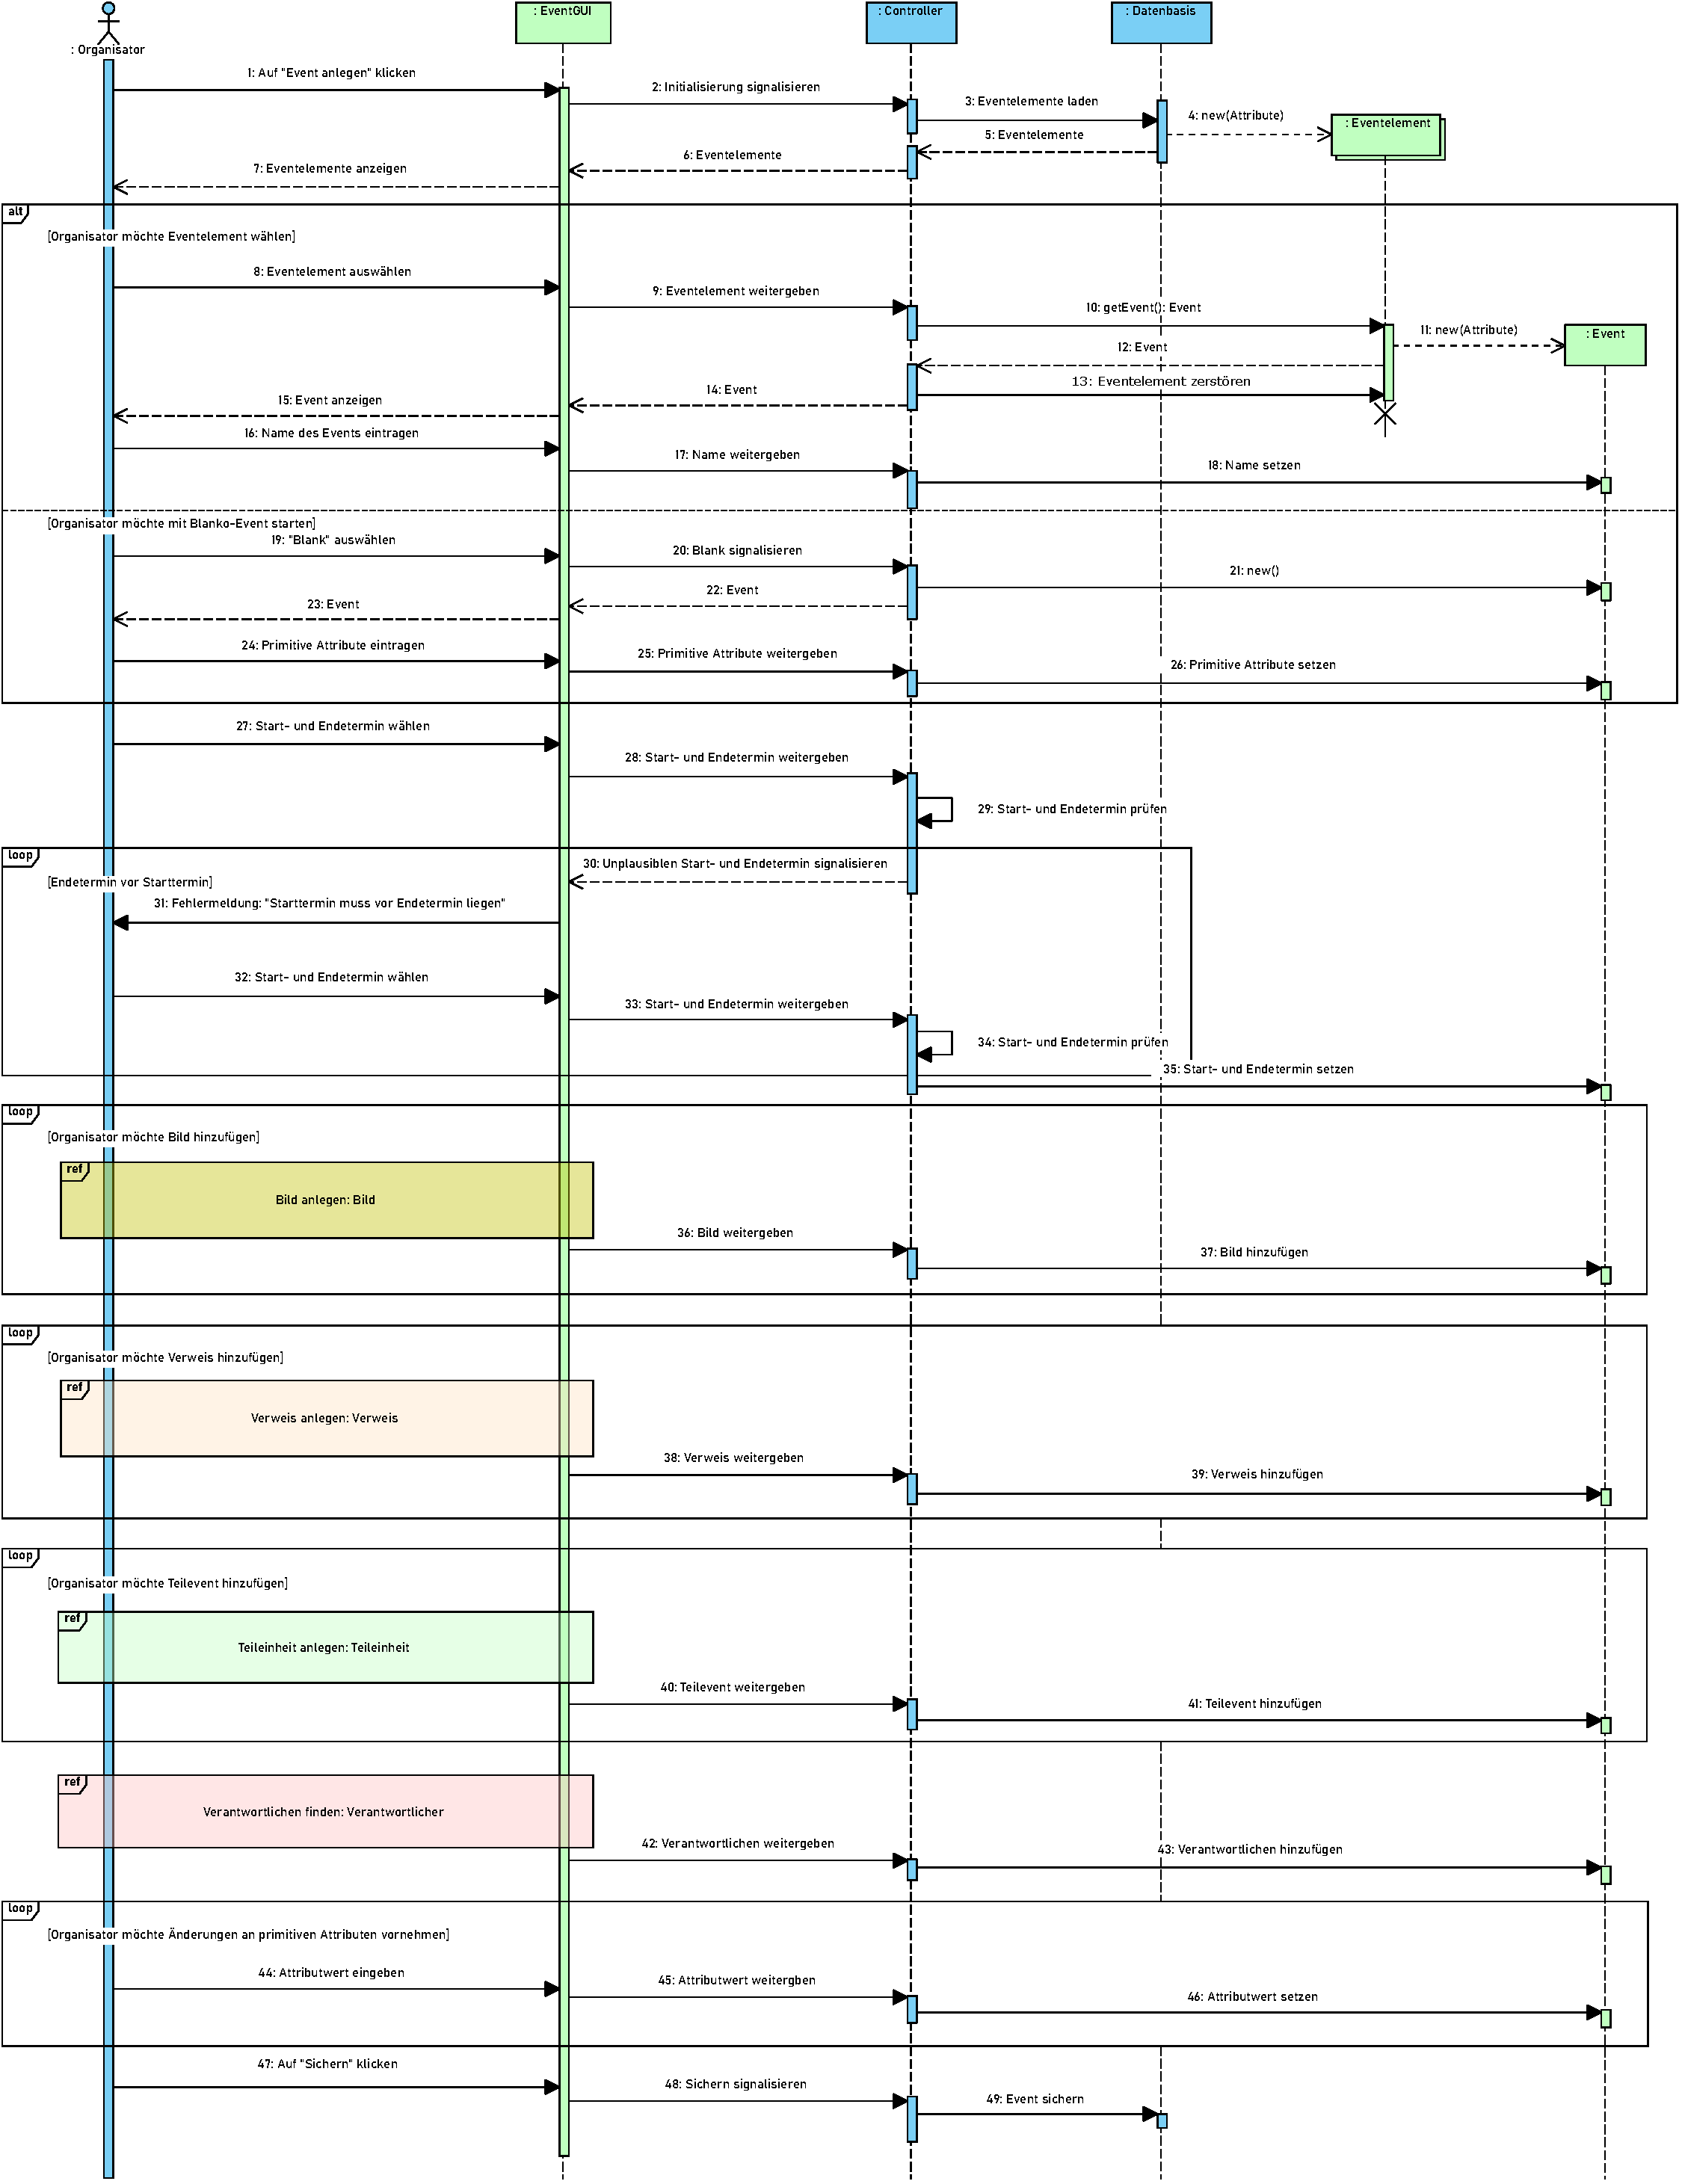
\includegraphics[width=0.98\columnwidth]{Bilder/seq_Event_anlegen.pdf}
    \caption{Szenario Event anlegen}
    \label{seq:event-anlegen}
\end{figure}

Das in \autoref{seq:event-anlegen} modellierte Szenario \enquote{Event anlegen} wird dadurch begonnen, dass der Organisator sich entschließt ein Event anzulegen und dieses dem System mitteilt. Zu Beginn muss entschieden werden, ob ein Eventelement als Vorlage verwendet werden soll oder mit einem leeren Event gestartet wird. Dafür werden zuerst alle verfügbaren Eventelemente aus der Datenbasis geladen und dem Nutzer angezeigt.

Möchte der Organisator mit einem Eventelement als Vorlage starten, so wählt er eine dieser Optionen und es beginnt der Prozess, aus dieser Vorlage ein Event zu erstellen. Jegliche primitiven Attribute des Eventelementes sowie alle dem Eventelement zugewiesenen Objekte werden dem neuen Event bei der Erschaffung direkt zugewiesen. Lediglich der Name muss durch den Nutzer noch manuell gesetzt werden, um zu vermeiden, dass sehr viele Events mit dem Namen des Eventelementes erstellt werden, denn generische Namen helfen dem Nutzer nicht, das Event von anderen zu unterscheiden.

Möchte der Organisator stattdessen mit einem leeren Eventobjekt starten, so wird zuerst ein leeres Eventobjekt erstellt, welches vom Organisator manuell mit primitiven Attributen befüllt werden muss. In beiden Fällen ist jetzt ein Eventobjekt vorhanden, welches vollständig befüllte primitive Attribute besitzt.

Anschließend werden Start- und Endetermin des Events vom Organisator eingetragen. Sollte der Endetermin vor dem Starttermin liegen, wird der Nutzer mit einer Fehlermeldung darüber unterrichtet. Diese Bedingung wird in einer Schleife wiederholt geprüft, bis der Fehler korrigiert wurde. Abschließend können dieser Start- und Endetermin gesetzt werden.

Das Hinzufügen der Objekte Teileinheit, Verweis und Bild ist hier auf gleiche Weise dargestellt. Es wird jeweils solange in einer Schleife verweilt, bis alle Objekte des gleichen Typs angelegt wurden. In der Schleife wird durch eine Interaktionsreferenz gezeigt, dass auf ein Unterprogramm verwiesen wird. Diese sind jeweils in den weiteren Diagrammen verfeinert dargestellt. Das Unterprogramm gibt jeweils ein Objekt des entsprechenden Typs zurück, welches dann zum Eventobjekt hinzugefügt wird.

Nachdem dieses getan ist, wird noch der Verantwortliche gesetzt. Dafür wird in einem Unterprogramm der Verantwortliche gefunden und anschließend hier nur noch als solcher im Eventobjekt gesetzt.

Zum Schluss kann der Organisator noch Änderungen an Attributen des Eventobjektes vornehmen, solange dieses nötig ist. Diese werden jeweils auf dem Eventobjekt gesetzt. Ist der Organisator vorerst fertig mit dem Bearbeiten des Events, so bestätigt er die Sicherung des Events. Dieses führt dazu, dass das Event auf der Datenbasis gesichert und damit persistent gespeichert wird.

\FloatBarrier

\subsection{Teileinheit anlegen}

\begin{figure}[ht!]
    \centering
    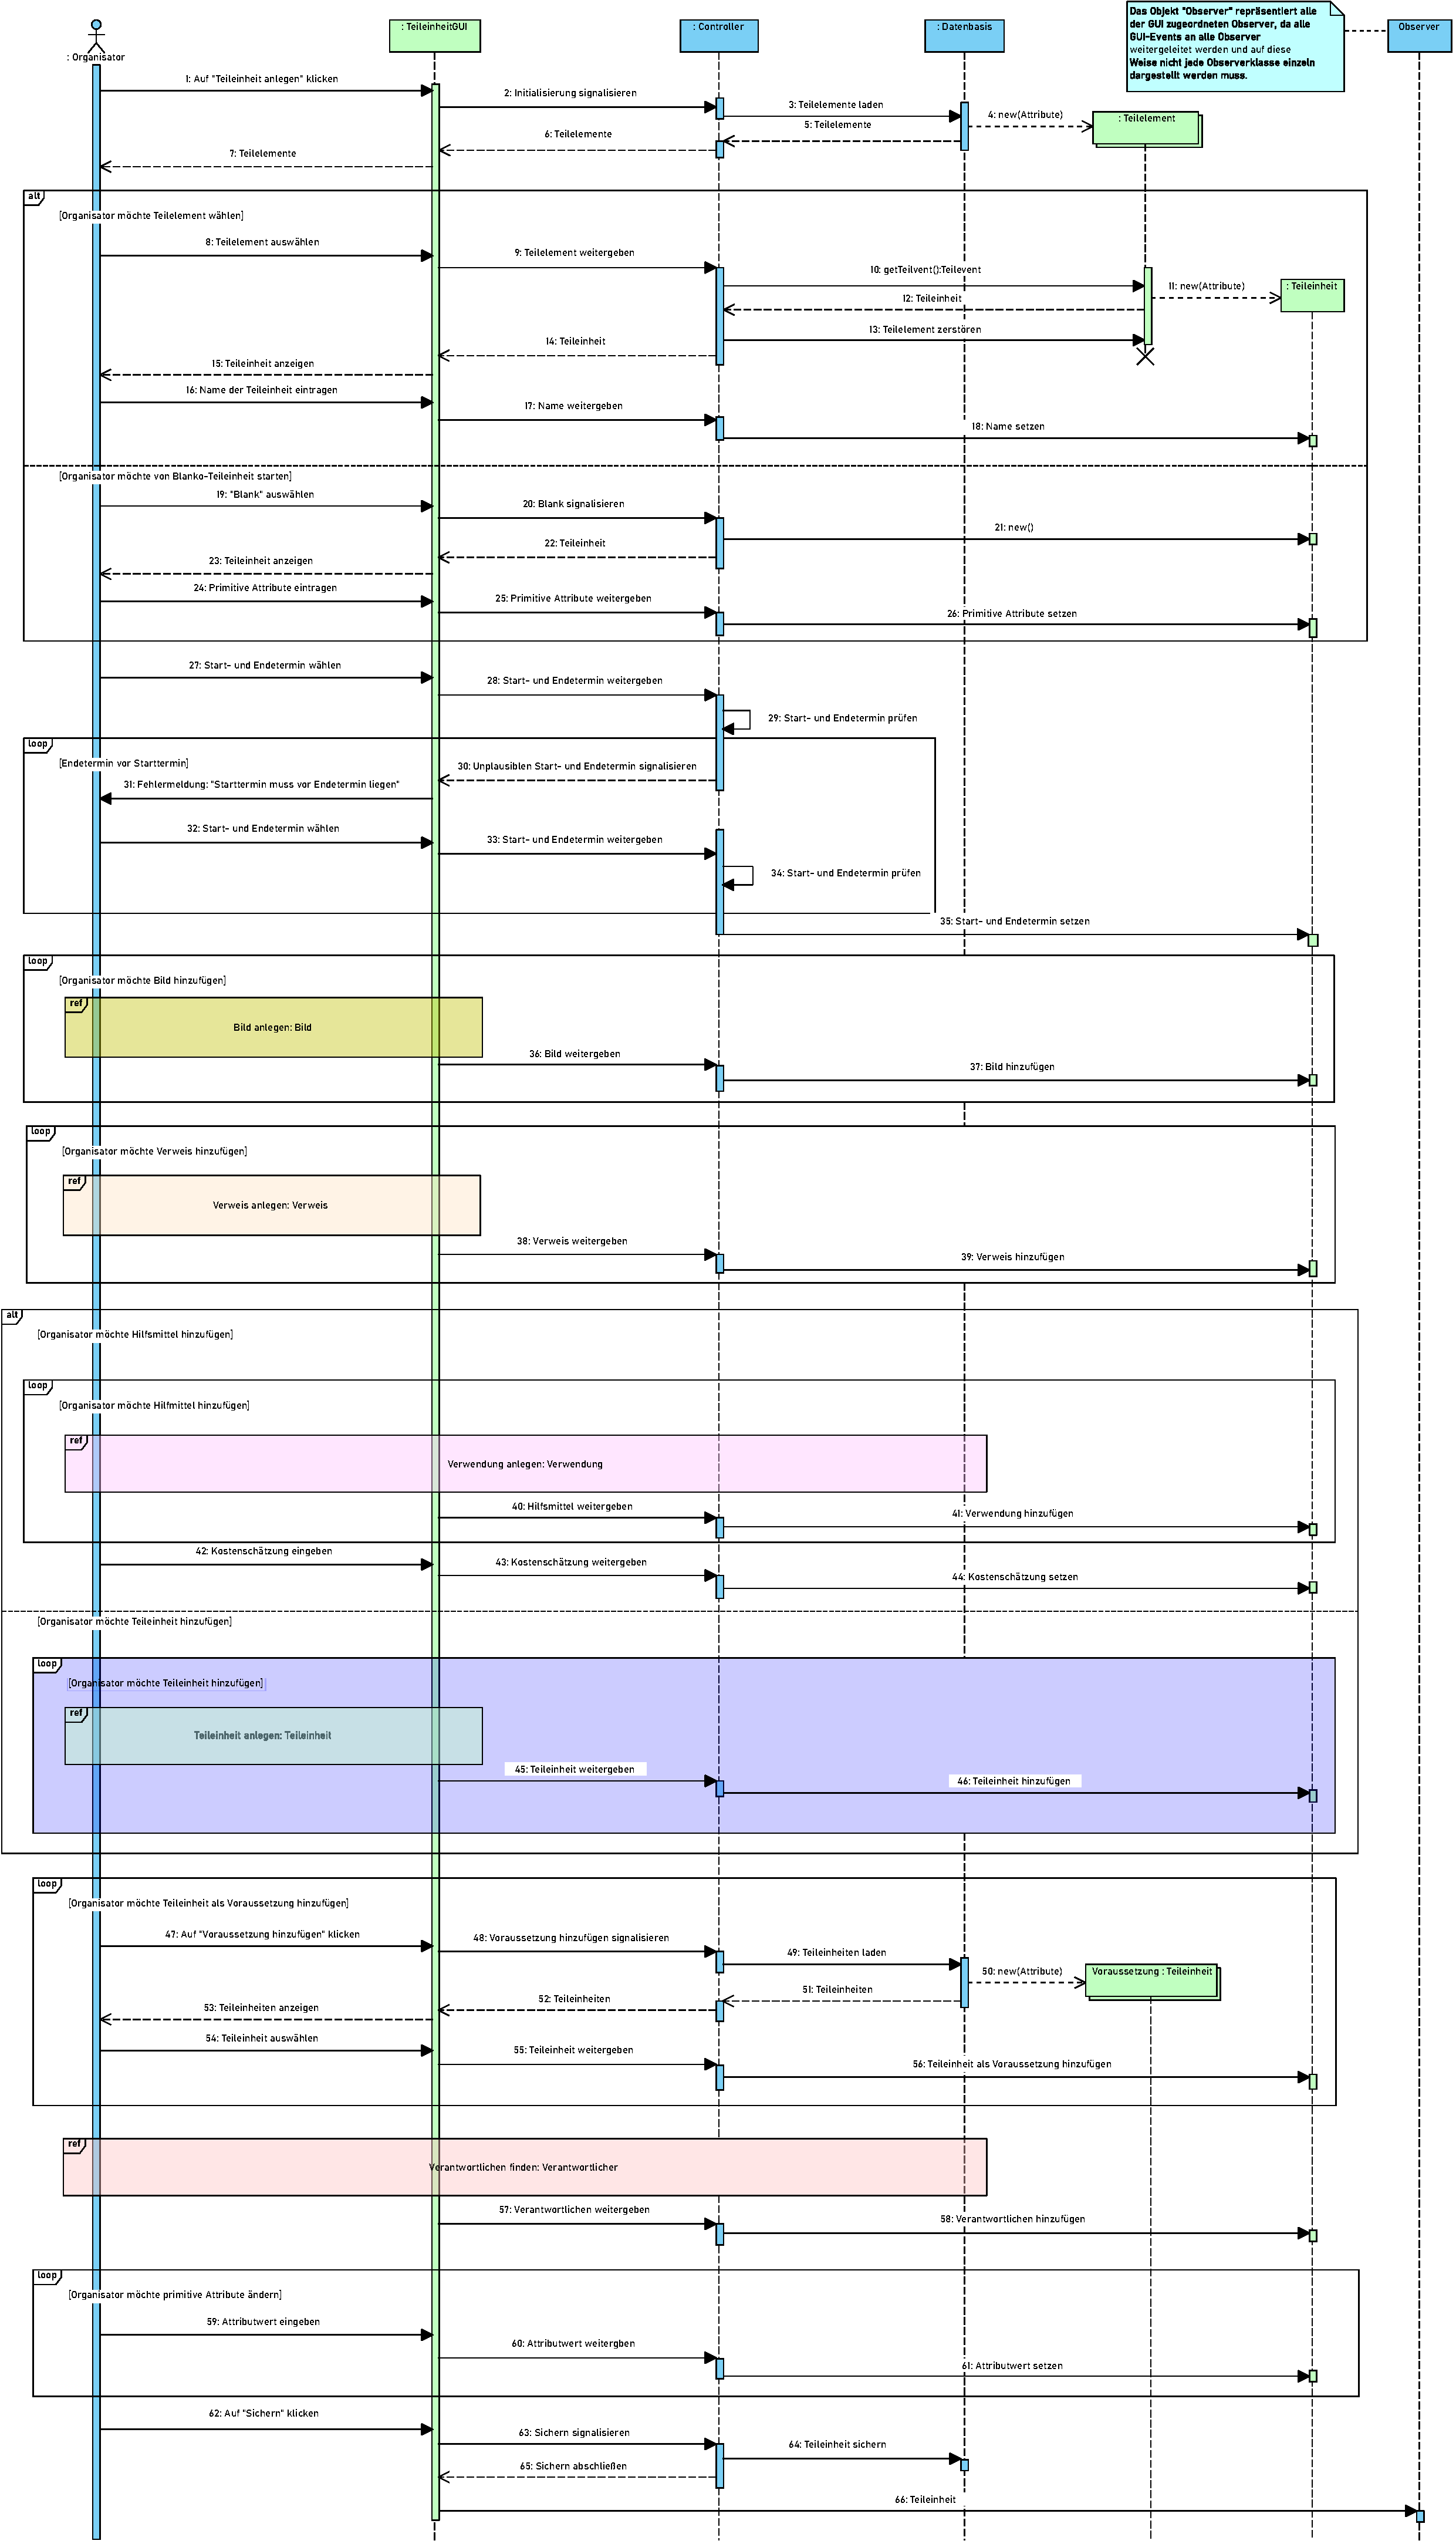
\includegraphics[width=0.7\columnwidth]{Bilder/seq_Teilevent_anlegen.pdf}
    \caption{Szenario Teileinheit anlegen}
    \label{seq:teileinheit-anlegen}
\end{figure}

Das Anlegen einer Teileinheit wurde in \autoref{seq:teileinheit-anlegen} modelliert. Hier klickt der Organisator zunächst auf \enquote{Teileinheit anlegen}, anschließend werden alle verfügbaren Teilelemente geladen und dem Organisator angezeigt. Nun hat der Organisator folgende mittels eines alt-Fragments modellierte Möglichkeiten: Im ersten Fall kann er die neue Teileinheit auf Basis eines der angezeigten Teilelemente erstellen, indem er dieses auswählt. In diesem Fall wird dann ein Teileinheitobjekt auf dem Teilelement generiert, anschließend werden die beim Laden erzeugten Teilelementobjekt zerstört. Nun muss der Organisator nur noch den Namen der Teileinheit eintragen, dann wird ihm die neue Teileinheit angezeigt. Im zweiten Fall, bei dem der Organisator kein Teilelement auswählt, wird mittels eines Konstruktoraufrufs eine leere Teileinheit erzeugt und dem Organisator angezeigt, sodass er die Möglichkeit hat, die primitiven Attribute der Teileinheit zu befüllen, welche anschließend im Teileinheitobjekt gesetzt werden.

Die folgenden Schritte sind nun wieder für beide der oben beschriebenen Pfade identisch. Zunächst wählt der Organisator einen Start- und einen Endetermin. Liegt der Starttermin vor dem Endetermin wird ihm eine Fehlermeldung angezeigt und er wird aufgefordert, einen neuen Start- und Endetermin auszuwählen. Dieser Vorgang wiederholt sich solange, bis der Starttermin vor dem Endetermin liegt, daher wurde diese Aktion als loop-Fragment modelliert.

Als nächstes hat der Organisator die Möglichkeit, der Teileinheit Bilder und Verweise hinzuzufügen. Hierzu müssen die Bild- und Verweisobjekte jedoch erst angelegt werden. Diese beiden Szenarien wurden allerdings in separaten Sequenzdiagrammen modelliert, welche hier mit Hilfe von Interaktionsreferenzen aufgerufen werden. Da der Organisator einer Teileinheit Bilder und Verweise in beliebiger Anzahl hinzufügen kann, finden das Anlegen und hinzufügen der Verweis- und Bildobjekte jeweils innerhalb eines loop-Fragmentes statt.

Im nächsten Schritt muss der Organisator wählen: Er kann der Teileinheit entweder weitere untergeordnete Teileinheiten hinzufügen oder er kann der Teileinheit Hilfsmittel hinzufügen. Diese beiden Möglichkeiten wurden durch ein alt-Fragment modelliert. Möchte der Organisator Hilfsmittel hinzufügen, so wird das Sequenzdiagramm \enquote{Verwendung anlegen} mittels einer Interaktionsreferenz aufgerufen und die entstandene Verwendung der Teileinheit hinzugefügt. Wie auch bei den Bildern und Verweisen, können einer Teileinheit beliebig viele Hilfsmittel hinzugefügt werden, daher befindet sich auch dieser Vorgang in einem loop-Fragment. Entscheidet sich der Organisator für das Hinzufügen weiterer Teileinheiten, müssen auch diese zuerst angelegt werden. Dies geschieht mittels eines rekursiven Aufrufs des hier beschrieben Sequenzdiagramms \enquote{Teileinheit anlegen}. Nun kann die erstellte Teileinheit der aktuellen hinzugefügt werden. Da jede Teileinheit beliebig viele Teileinheiten besitzen kann, befinden sich auch diese beiden Vorgänge innerhalb eines loop-Fragments.

Da Teileinheiten auch von einander abhängig sein können, hat der Organisator nun die Möglichkeit, vorhandene Teileinheiten als Voraussetzung für die aktuelle hinzuzufügen. Hierzu klickt er auf \enquote{Teileinheit als Voraussetzung hinzufügen}. Anschließend werden die vorhandenen Teileinheiten aus der Datenbasis geladen und angezeigt, sodass er die Möglichkeit hat, die gewünschte Teileinheit auszuwählen, welche der aktuellen dann als Voraussetzung hinzugefügt wird. Auch dieser Vorgang kann sich beliebig oft wiederholen und befindet sich darum in einem loop-Fragment.

Als nächstes muss ein Verantwortlicher für die Teileinheit gefunden werden. Dies geschieht mittels einer Interaktionsreferenz auf das Sequenzdiagramm \enquote{Verantwortlichen finden}. Der gefundene Verantwortliche, bei dem es sich sowohl um einen einzelnen Mitarbeiter, als auch um eine Gruppe von Mitarbeiter handeln kann, wird der Teileinheit als Verantwortlicher hinzugefügt.

Zuletzt hat der Organisator noch einmal die Möglichkeit, die primitiven Attribute der Teileinheit zu ändern. Dies kann beliebig oft geschehen und findet darum in einem loop-Fragment statt. Hierzu gibt der Organisator den neuen Attributwert ein, welcher anschließend in der Teileinheit gesetzt wird.
Abschließend klickt der Organisator auf \enquote{sichern}, sodass diese in der Datenbasis gespeichert wird.

\FloatBarrier

\subsection{Verantwortlichen finden}

\begin{figure}[ht!]
    \centering
    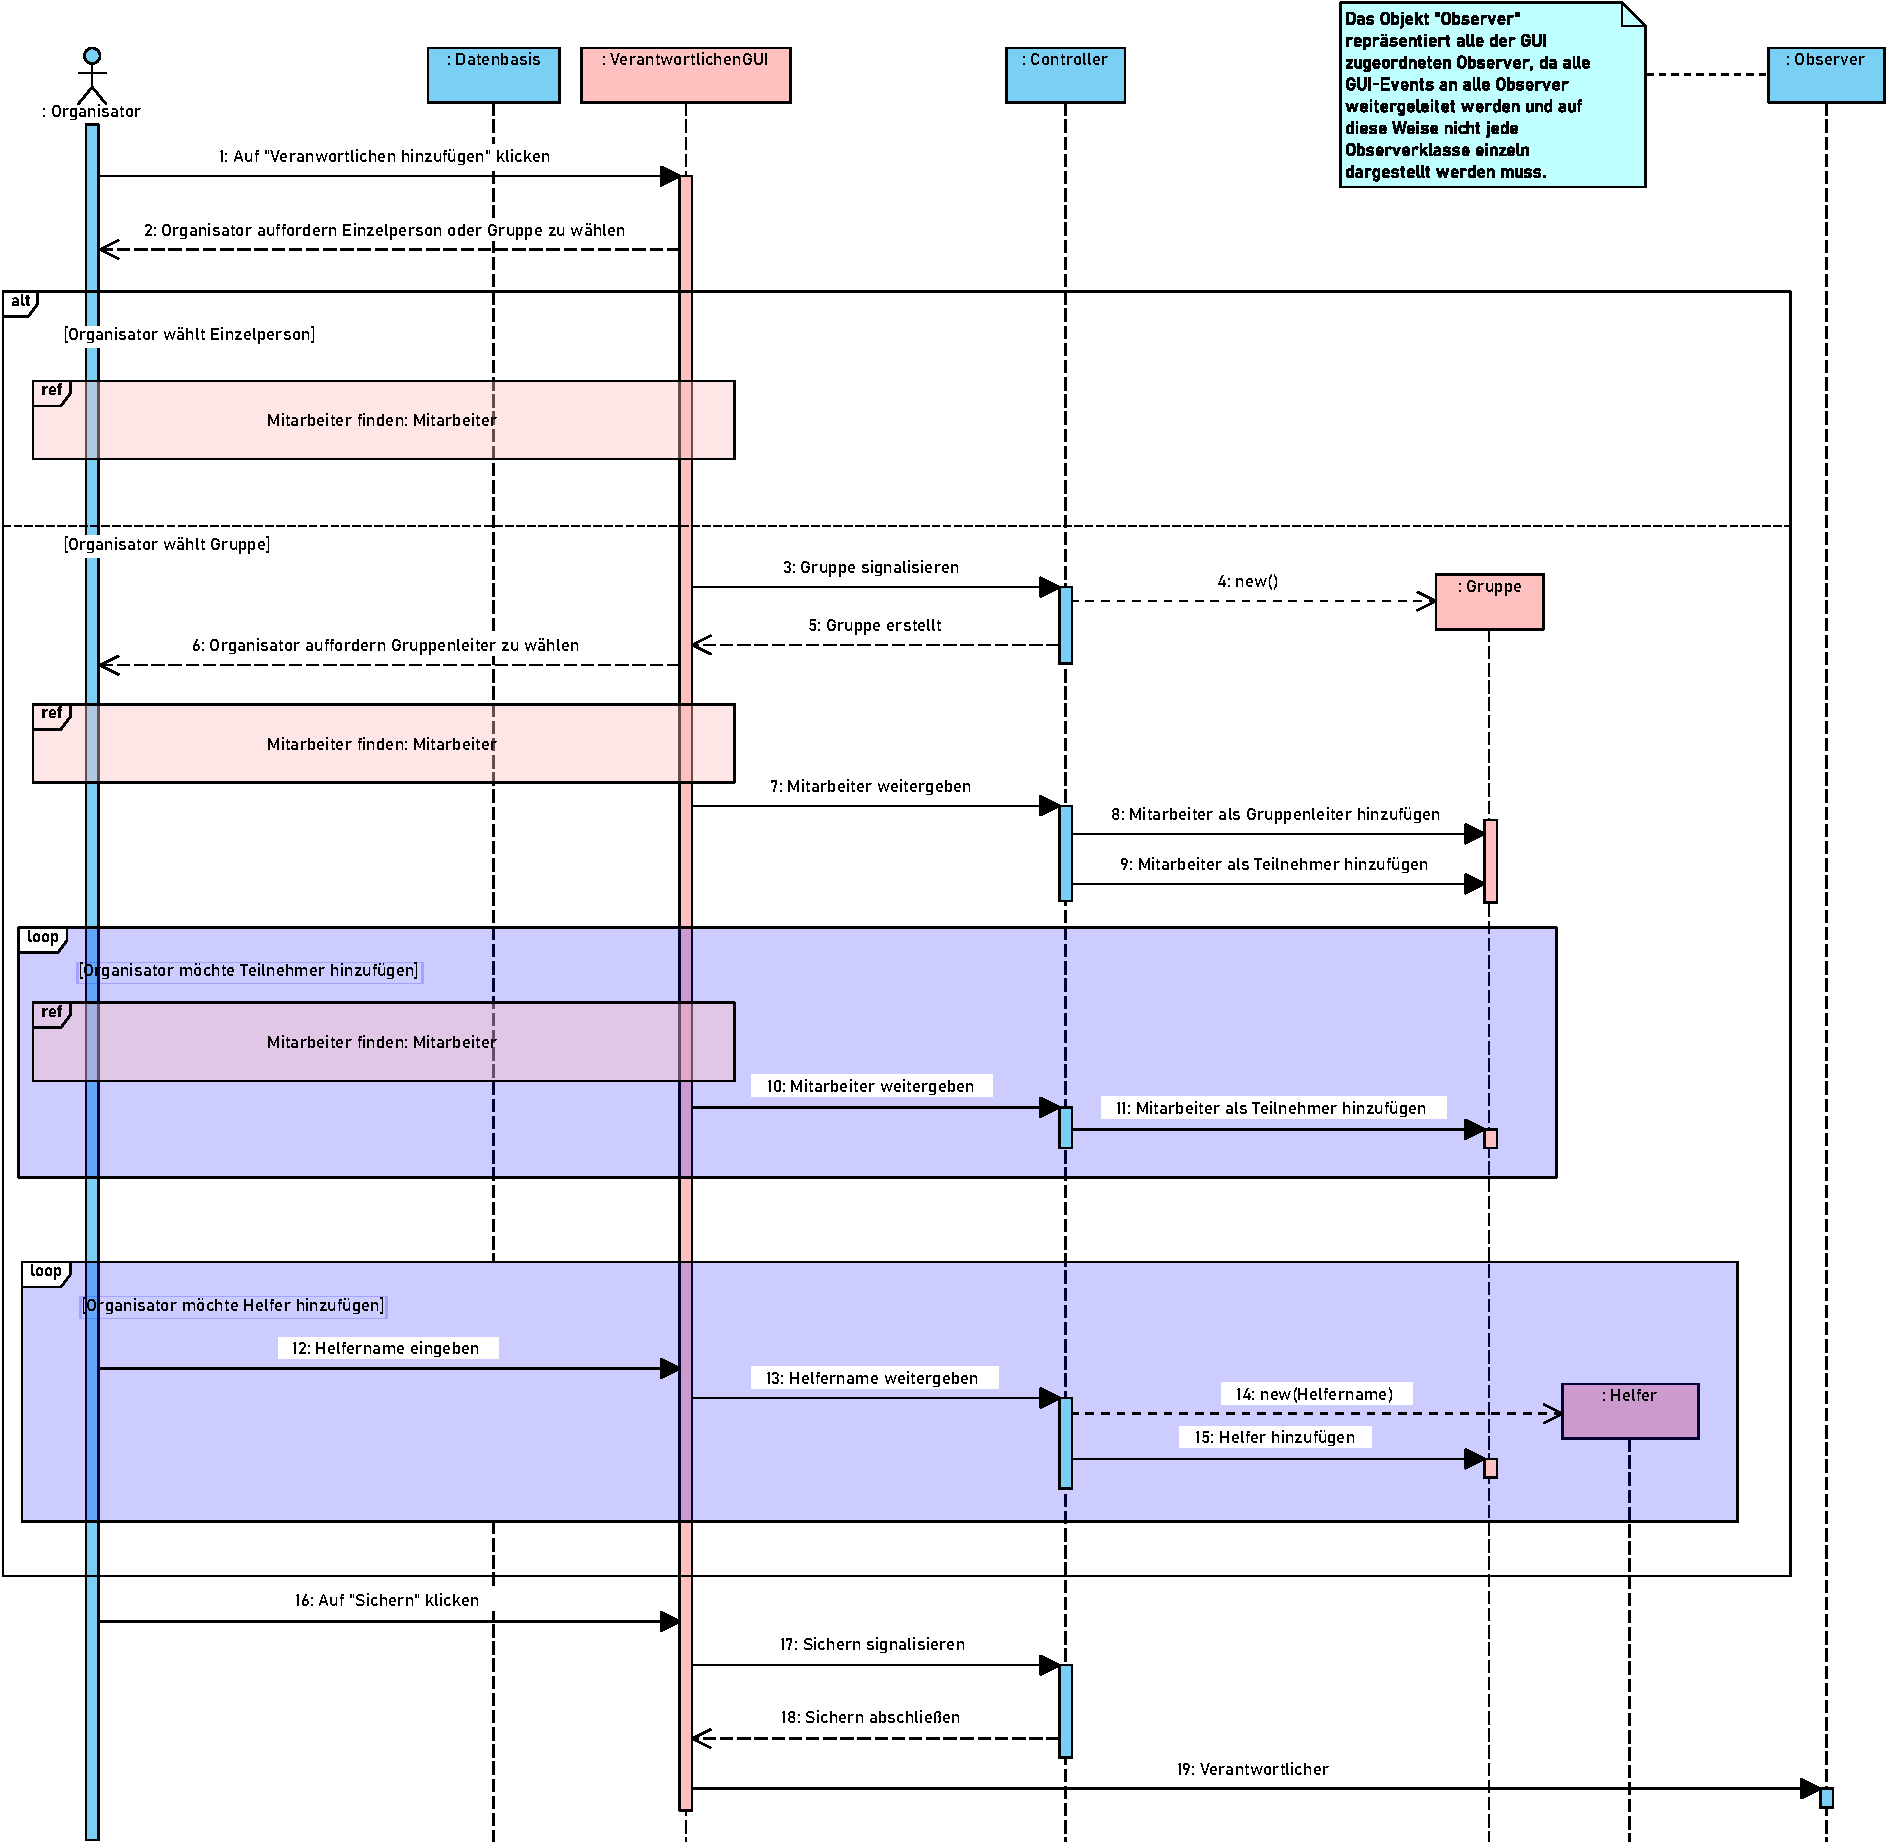
\includegraphics[width=0.98\columnwidth]{Bilder/seq_Verantwortlichen_finden.pdf}
    \caption{Szenario Verantwortlichen finden}
    \label{seq:verantwortlichen-finden}
\end{figure}

Beim Finden eines Verantwortlichen, was in \autoref{seq:verantwortlichen-finden} modelliert wurde, wird der Organisator zunächst aufgefordert, zu wählen, ob es sich bei dem Verantwortlichen um eine Gruppe oder eine Einzelperson handeln soll. Von hier an gibt es zwei mögliche Pfade: Entscheidet sich der Organisator für eine Einzelperson, so wird das Sequenzdiagramm \enquote{Mitarbeiter finden} mittels einer Interaktionsreferenz aufgerufen. Im zweiten Fall, wenn der Organisator sich für eine Gruppe als Verantwortlichen entscheidet, wird zunächst ein neues Gruppenobjekt erzeugt und der Organisator aufgefordert, einen Gruppenleiter zu bestimmen. Auch dies geschieht mit Hilfe des Sequenzdiagramms \enquote{Mitarbeiter finden}. Der so gefundene Mitarbeiter wird dem Gruppenobjekt dann sowohl als Gruppenleiter als auch als Teilnehmer hinzugefügt. Nun können der Gruppe noch beliebig viele weitere Teilnehmer hinzugefügt werden. Darum finden die beiden folgenden Schritte in einem loop-Fragment statt: Zunächst wird das Sequenzdiagramm \enquote{Mitarbeiter hinzufügen} aufgerufen. Der gefundene Mitarbeiter wird dann dem Gruppenobjekt als Teilnehmer hinzugefügt. Zuletzt hat der Organisator noch die Möglichkeit der Gruppe externe Helfer hinzuzufügen. Hierzu muss der Organisator lediglich den Namen des Helfers eingeben, anschließend wird eines neues Helferobjekt erzeugt, welches dann dem Gruppenobjekt hinzugefügt wird. Da in einer Gruppe auch beliebig viele Helfer sein können, findet auch dieser Vorgang innerhalb eines loop-Fragments statt. 

\FloatBarrier

\subsection{Mitarbeiter finden}

\begin{figure}[ht!]
    \centering
    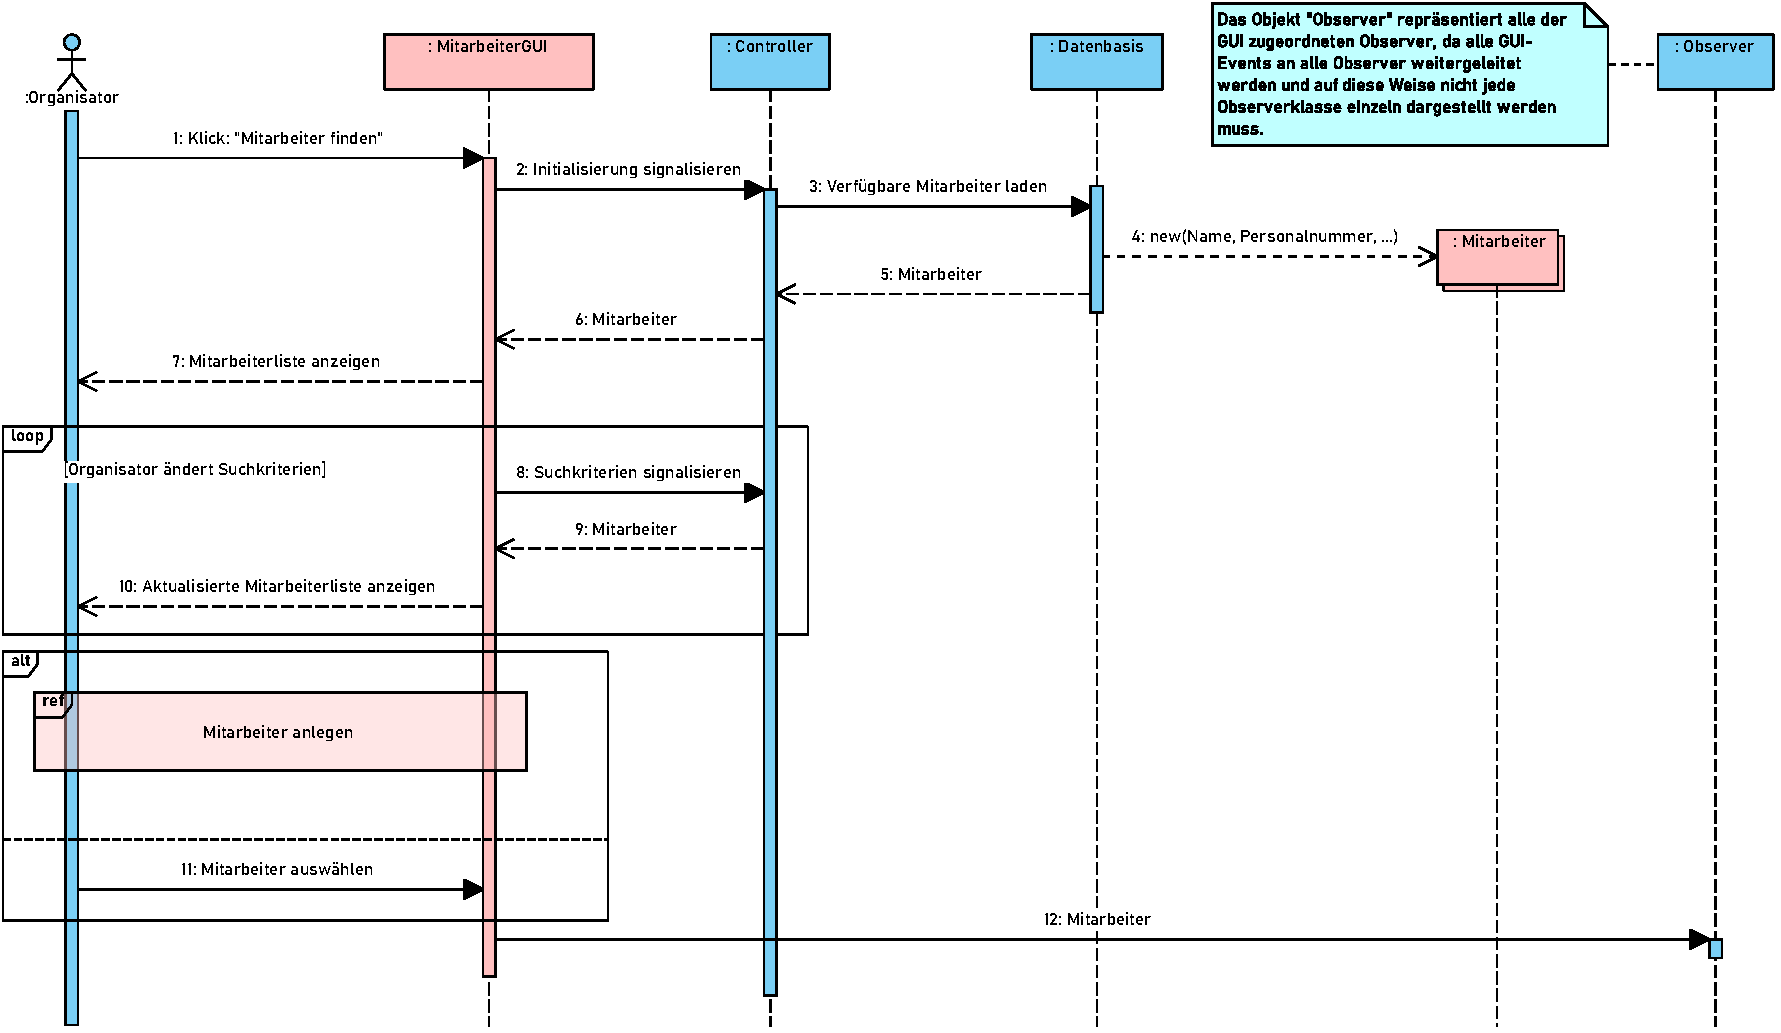
\includegraphics[width=0.98\columnwidth]{Bilder/seq_Mitarbeiter_finden.pdf}
    \caption{Szenario Mitarbeiter finden}
    \label{seq:mitarbeiter-finden}
\end{figure}

Um einen Mitarbeiter zu finden, klickt der Organisator zunächst auf \enquote{Mitarbeiter finden} wie man in \autoref{seq:mitarbeiter-finden} erkennen kann. Anschließend werden alle zwischen Start- und Endetermin verfügbaren Mitarbeiter aus der Datenbasis geladen und dem Organisator angezeigt. Nun kann der Organisator die verfügbaren Mitarbeiter nach ihren Attributen filtern. Hierzu ändert er die Suchkriterien, dann wird ihm eine aktualisierte Liste der Mitarbeiter angezeigt. Dieser Vorgang wiederholt sich, so oft der Organisator die Suchkriterien ändert, weshalb sich dieser in einem loop-Fragment befindet.

Nun gibt es zwei Möglichkeiten: Hat der Organisator einen passenden Mitarbeiter gefunden, wählt er diesen aus. Findet er keinen passenden Mitarbeiter, kann ein neuer angelegt werden und das Sequenzdiagramm \enquote{Mitarbeiter anlegen} wird aufgerufen.

\FloatBarrier
\newpage

\subsection{Verweis anlegen}

\begin{figure}[ht!]
    \centering
    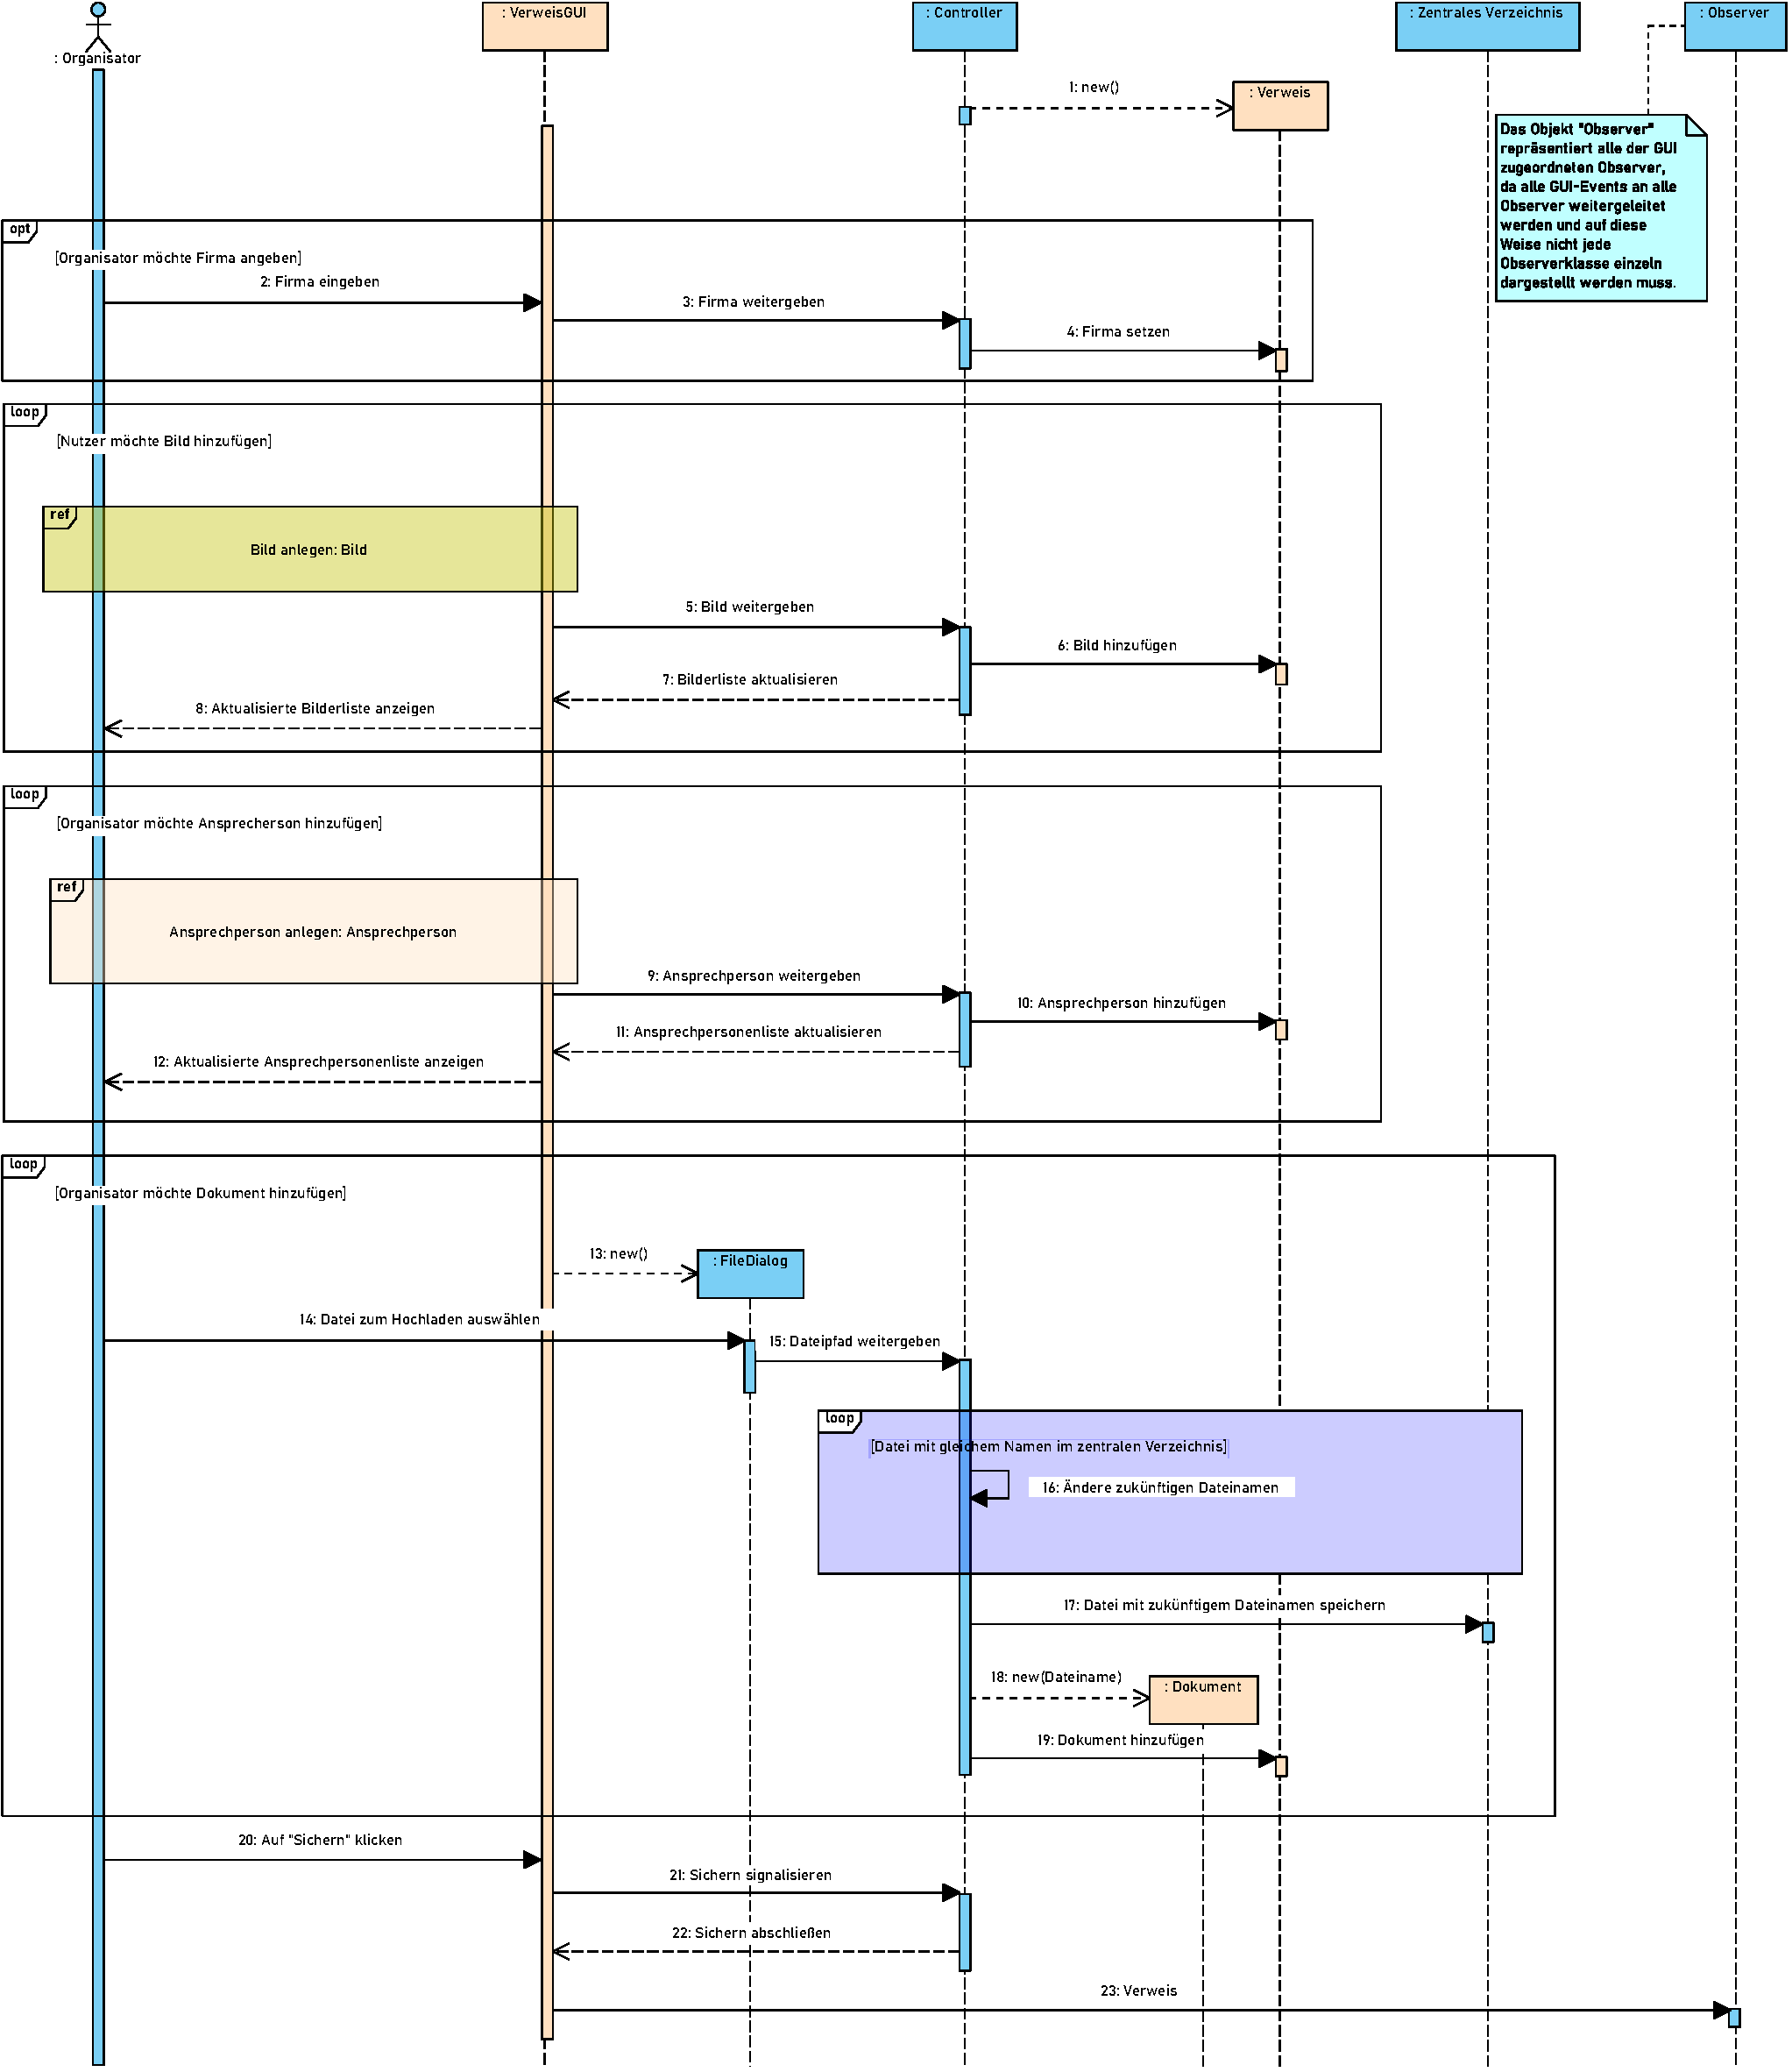
\includegraphics[width=0.98\columnwidth]{Bilder/seq_Verweis_anlegen.pdf}
    \caption{Szenario Verweis anlegen}
    \label{seq:verweis-anlegen}
\end{figure}

\FloatBarrier

Das Szenario \enquote{Verweis anlegen} ist in \autoref{seq:verweis-anlegen} dargestellt. Besonders am Verweisobjekt ist, dass jegliche seiner Attribute optional sind und es nicht alleine vorhanden sein kann. Daher wird das Objekt nicht zum Ende selbst in der Datenbasis, sondern nur als Teil des Events gesichert.

Zu Beginn des Szenarios wird ein vollständig leeres Verweisobjekt angelegt. Es besteht die Option, eine Firma anzugeben, zu der dieser Verweis gehört. Dieses primitive Attribut wird dann gesetzt.

Anschließend können in drei Schleifen die referenzierten Objekte Bild, Ansprechperson und Dokument angelegt und zum Verweis hinzugefügt werden. Das Bild und die Ansprechperson werden jeweils in anderen Unterprogrammen angelegt und hier dann nur noch zum Verweis hinzugefügt.

Da keine andere Entität Dokumente beinhalten kann, wurde sich dafür entschieden, das Anlegen eines Dokumentes nicht auf ein weiteres Unterprogramm auszulagern, sondern direkt hier zu beschreiben. Dazu wird vom Organisator eine Datei zum Hochladen ausgewählt. Es wird geprüft, ob im zentralen Verzeichnis bereits eine Datei mit dem gleichen Namen existiert. Sollte das der Fall sein, so wird der Name der Datei angepasst. Dieses wird in einer Schleife wiederholt, bis ein einzigartiger Name gefunden wurde. Dadurch wird garantiert, dass keine vorhandene Datei überschrieben wird. Wurde ein Name gefunden, so wird die Datei im zentralen Verzeichnis mit dem entsprechenden Namen abgelegt und ein Dokumentobjekt mit der Referenz auf diese Datei angelegt. Dieses Dokumentobjekt wird abschließend dem Verweis hinzugefügt.

\FloatBarrier
\newpage

\subsection{Bild anlegen}

\begin{figure}[ht!]
    \centering
    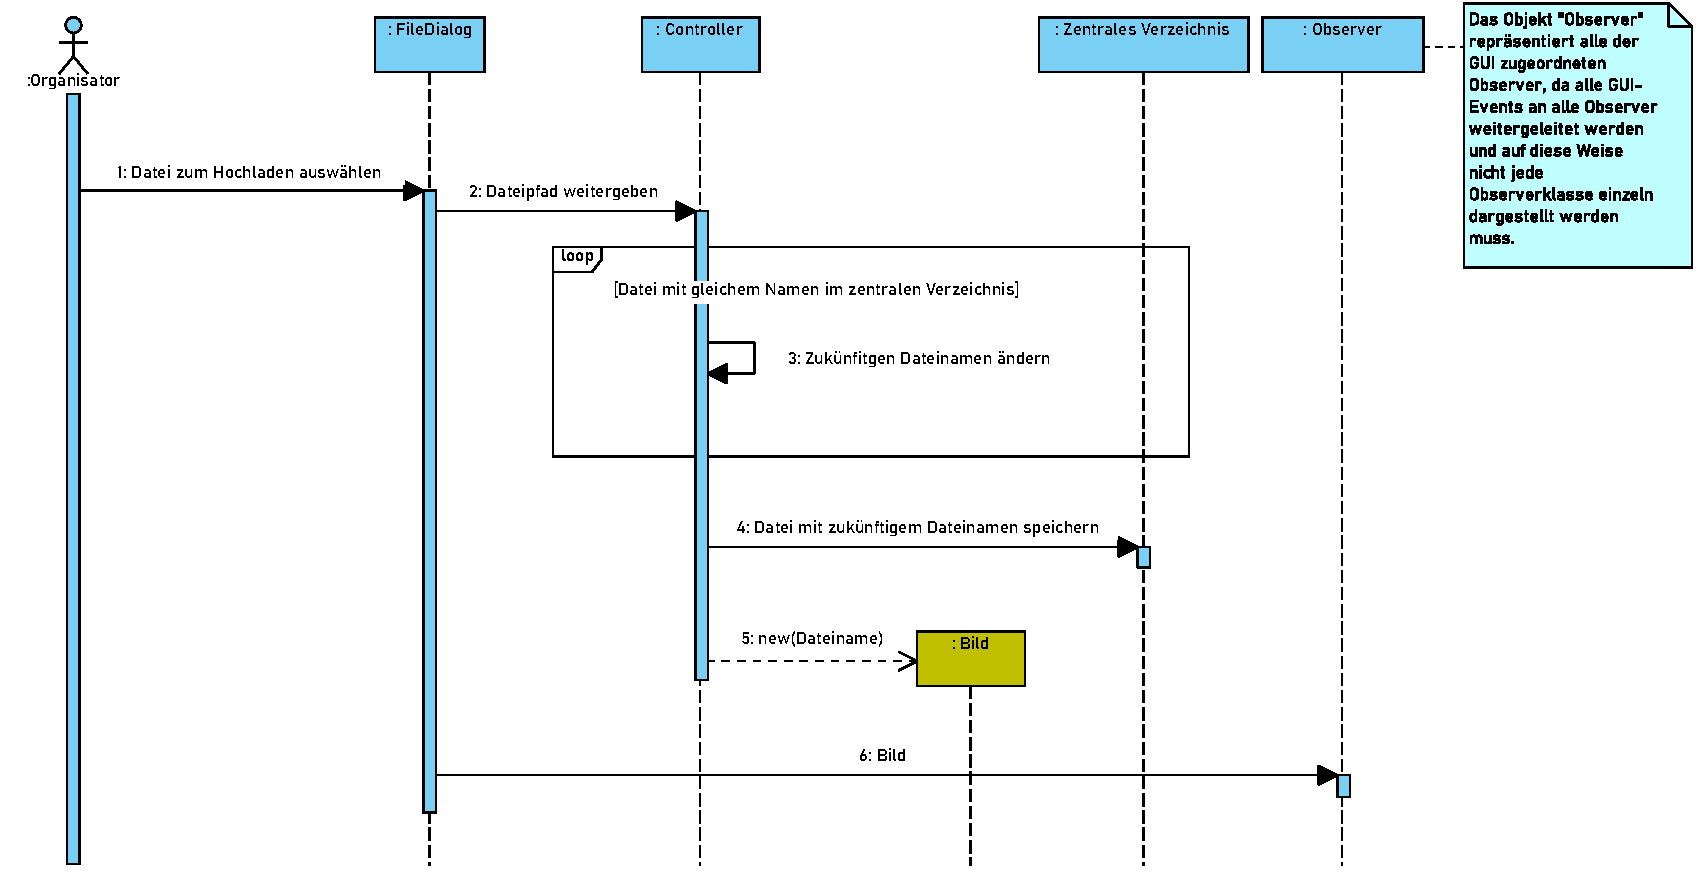
\includegraphics[width=0.98\columnwidth]{Bilder/seq_Bild_anlegen.pdf}
    \caption{Szenario Bild anlegen}
    \label{seq:bild-anlegen}
\end{figure}

In \autoref{seq:bild-anlegen} ist das Anlegen eines Bildes dargestellt. Dieses verläuft analog zu dem Prozess, ein Dokument anzulegen. Es wird ebenfalls eine Datei zum Hochladen gewählt, ein einzigartiger Name gefunden und anschließend die Datei im zentralen Verzeichnis abgelegt. Abschließend wird ein Bildobjekt mit Referenz auf die neu erstellte Datei erzeugt.

\FloatBarrier

\subsection{Ansprechperson anlegen}

In \autoref{seq:ansprechperson-anlegen} ist das Anlegen einer Ansprechperson dargestellt. Es werden zuerst die primitiven Attribute gesetzt und anschließend ein Kontaktdatenobjekt angelegt und dieses als Kontaktdaten der Ansprechperson gesetzt. Da die Telefonnummer ein verpflichtendes Attribut der Kontaktdaten ist, wird diese zu Beginn direkt vom Organisator eingegeben. Anschließend gibt es die Möglichkeit, die E-Mail-Adresse und die Anschrift anzugeben. Diese Möglichkeiten werden jeweils durch einen opt-Frame dargestellt. Zum Schluss wird das Kontaktdatenobjekt mit allen zuvor eingegebenen Daten erstellt.

\begin{figure}[ht!]
    \centering
    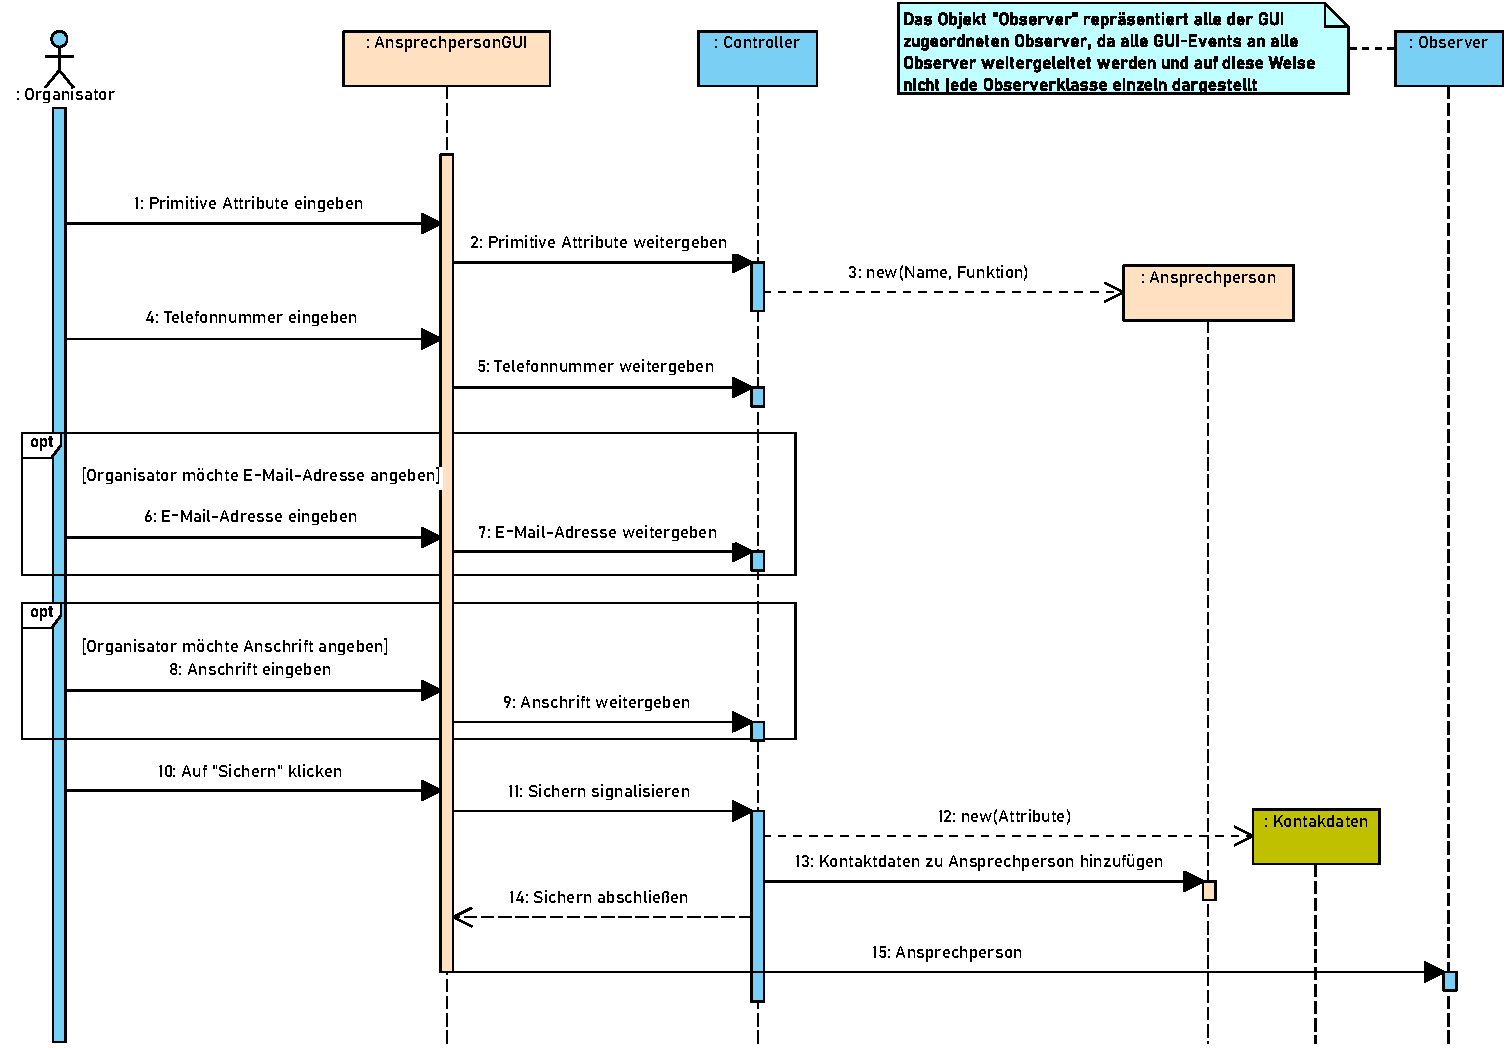
\includegraphics[width=0.98\columnwidth]{Bilder/seq_Ansprechperson_anlegen.pdf}
    \caption{Szenario Ansprechperson anlegen}
    \label{seq:ansprechperson-anlegen}
\end{figure}

\FloatBarrier

\subsection{Verwendung anlegen}

\begin{figure}[ht!]
    \centering
    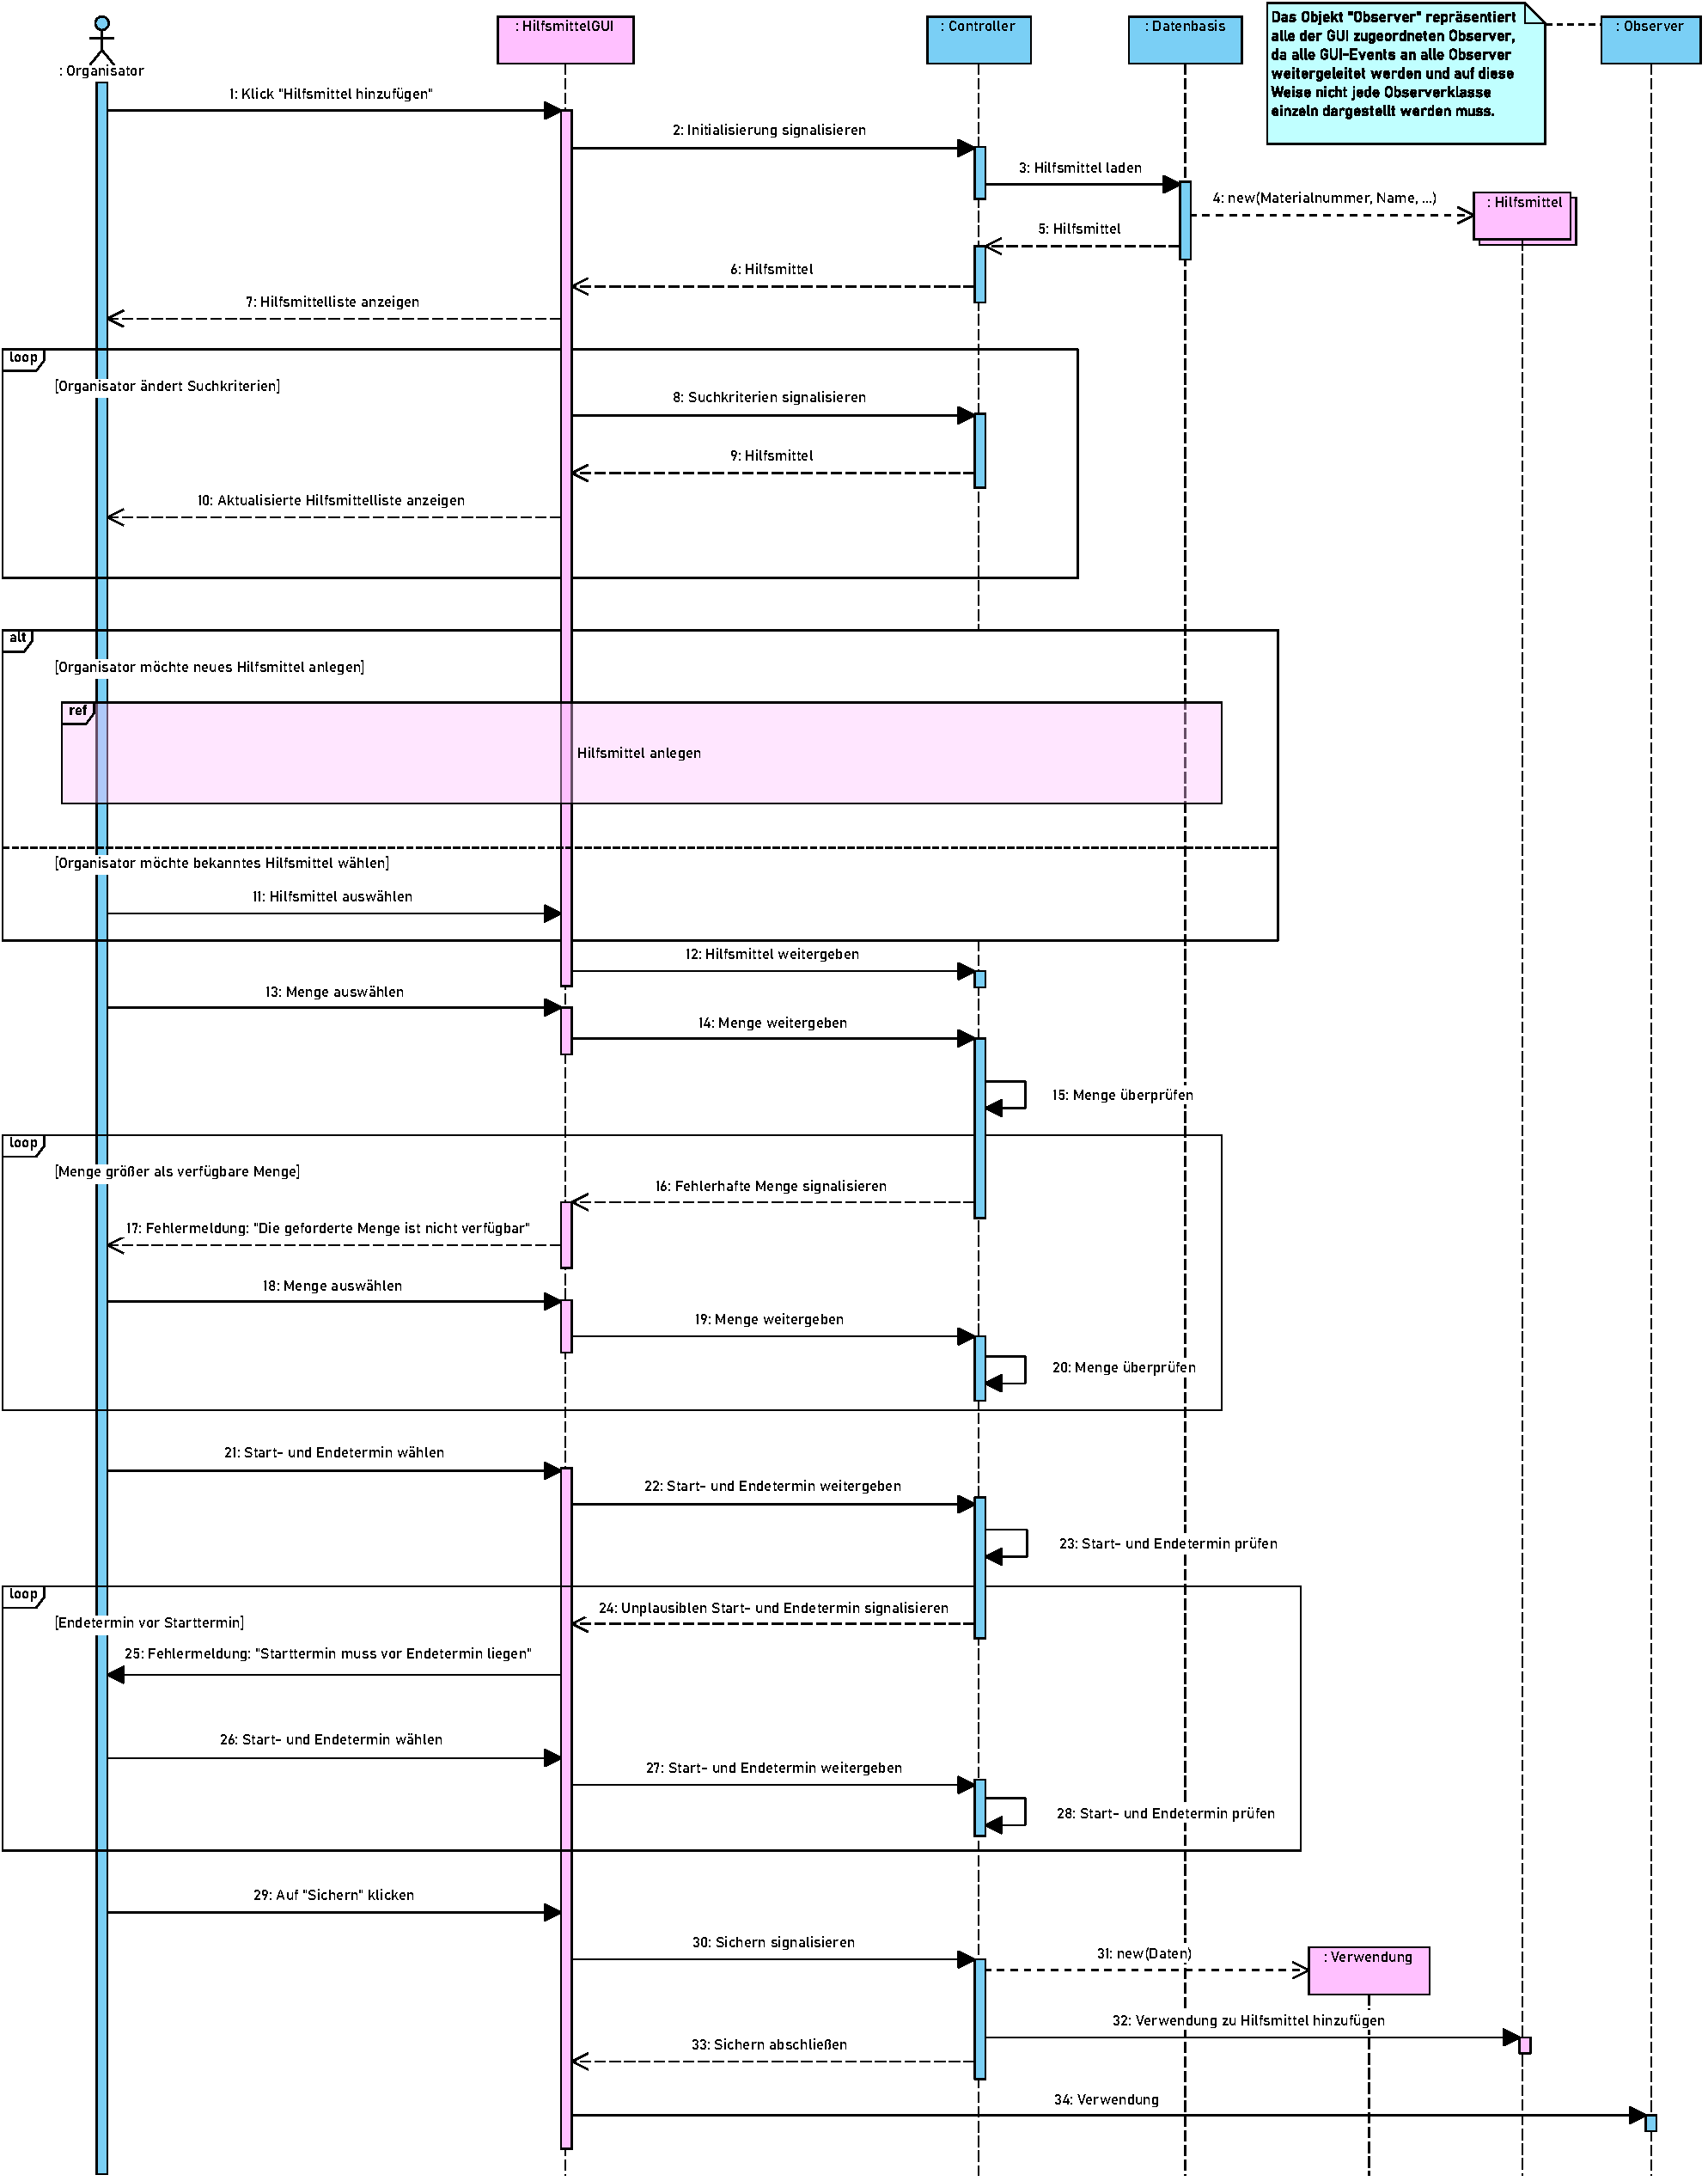
\includegraphics[width=0.9\columnwidth]{Bilder/seq_Verwendung_anlegen.pdf}
    \caption{Szenario Verwendung anlegen}
    \label{seq:verwendung-anlegen}
\end{figure}

Beim Anlegen einer Verwendung werden, wie in \autoref{seq:verwendung-anlegen} gezeigt, zunächst alle verfügbaren Hilfsmittel aus der Datenbasis geladen und dem Organisator als Liste angezeigt. Als nächstes kann der Organisator innerhalb eines loop-Fragments die Mitarbeiterliste filtern, in dem er beliebig oft die Sucherkriterien ändert und ihm eine aktualisierte Hilfsmittelliste angezeigt wird. Nun muss der Organisator wählen, ob er die Verwendung für ein neues oder ein vorhandenes Hilfsmittel anlegen möchte. Dieses wurde mit Hilfe eines alt-Fragmentes modelliert. Möchte er die Verwendung für ein neues Hilfsmittel anlegen, so wird das Sequenzdiagramm \enquote{Hilfsmittel anlegen} aufgerufen. Soll die Verwendung für ein vorhandenes Hilfsmittel sein, wählt er dieses aus der Hilfsmittelliste. Als nächstes muss die zu buchende Menge des Hilfsmittels gewählt werden. Ist die gewählte Menge größer als die vorhandene, wird eine Fehlermeldung angezeigt und der Organisator aufgefordert, eine kleinere Menge zu wählen. Dieses wiederholt sich in einem loop-Fragment solange, bis die gewählte Menge nicht mehr größer ist, als die vorhandene. Als letzte Attribute werden Start- und Endetermin gewählt. Auch hier wird solange eine Fehlermeldung gezeigt und der Organisator aufgefordert Start- und Endetermin zu ändern, bis Start- und Endetermin plausibel sind. Plausibel bedeutet in diesem Zusammenhang, dass Start- und Endetermin innerhalb des Zeitraums der Teileinheit liegen und der Starttermin vor dem Endetermin liegt. Schließlich wird ein neues Verwendungsobjekt aus den Eingaben erzeugt und dieses zu den Hilfsmitteln hinzugefügt.

\FloatBarrier

\subsection{Mitarbeiter anlegen}

\begin{figure}[ht!]
    \centering
    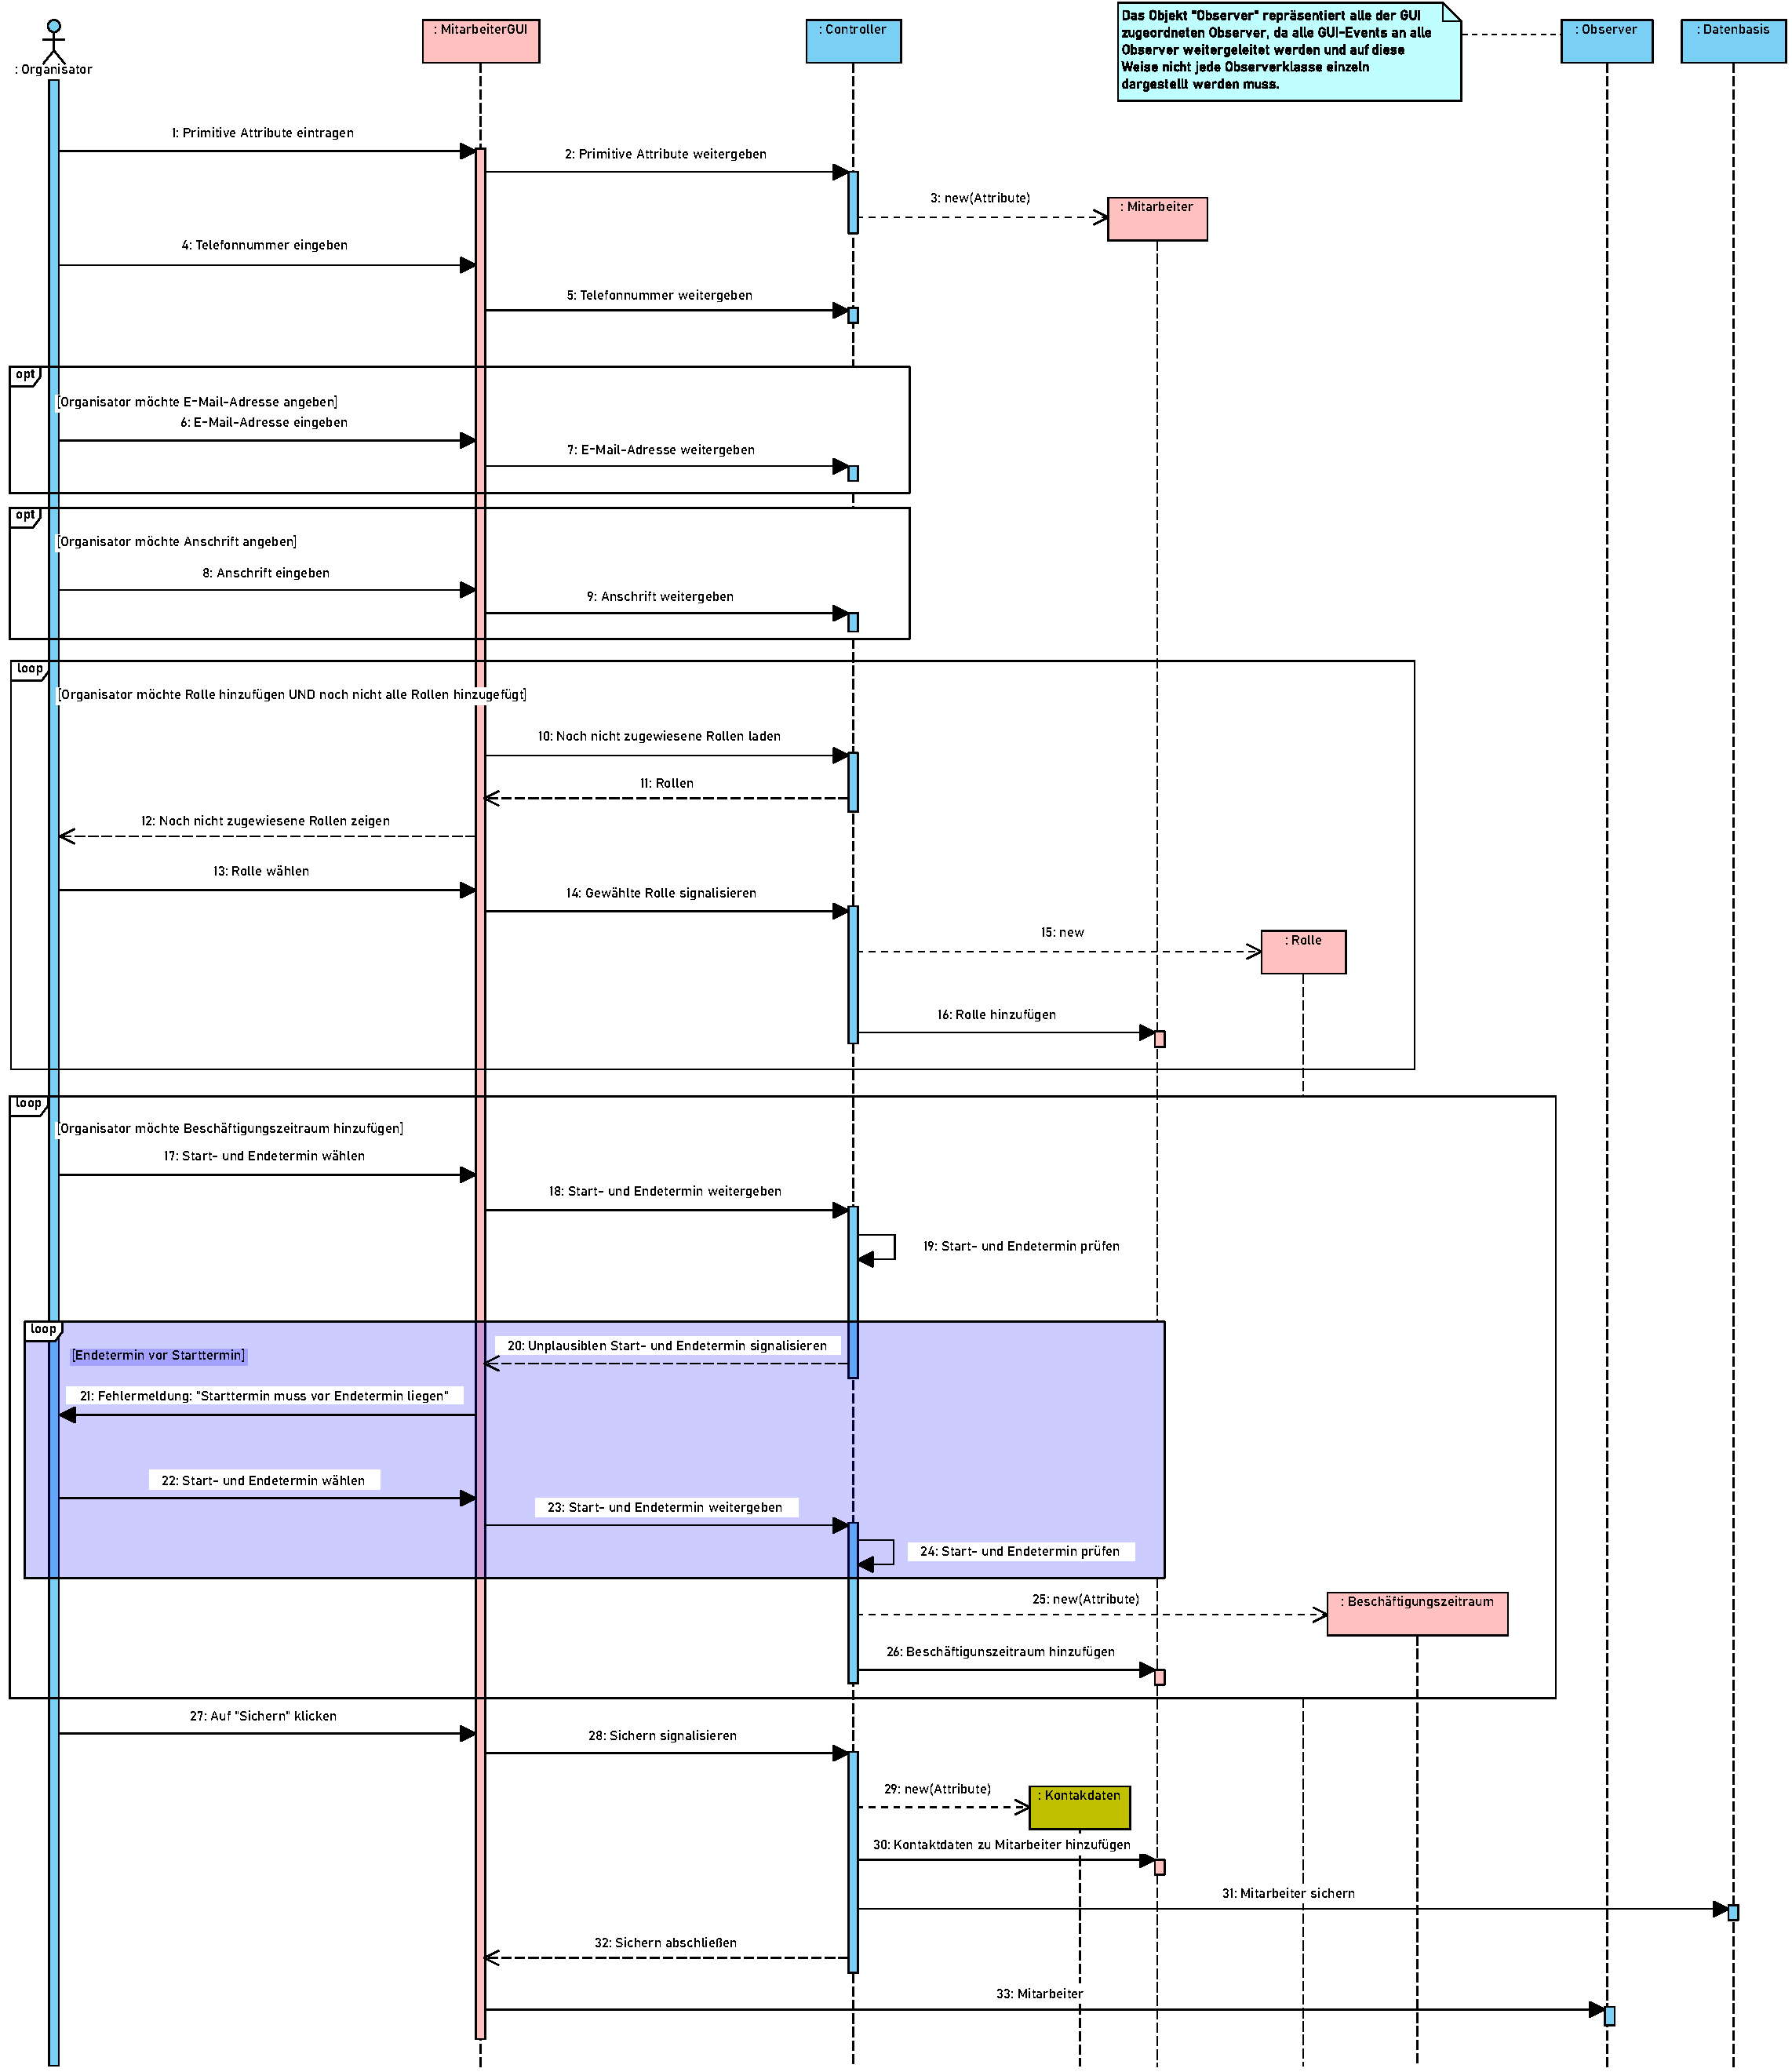
\includegraphics[width=0.98\columnwidth]{Bilder/seq_Mitarbeiter_anlegen.pdf}
    \caption{Szenario Mitarbeiter anlegen}
    \label{seq:mitarbeiter-anlegen}
\end{figure}

Das Anlegen eines Mitarbeiters wurde in \autoref{seq:mitarbeiter-anlegen} modelliert. Hier trägt der Organisator zunächst die primitiven Attribute des Mitarbeiters ein, aus denen dann ein Mitarbeiterobjekt erzeugt wird. Dann werden dessen Kontaktdaten hinterlegt. Hierzu wird ebenso vorgegangen wie in \autoref{seq:ansprechperson-anlegen} und dann das erstellte Kontaktdatenobjekt dem Mitarbeiterobjekt hinzugefügt. Als nächstes werden dem Mitarbeiter Rollen hinzugefügt. Dazu werden die dem Mitarbeiter noch nicht zugewiesenen Rollen angezeigt und der Organisator wählt die gewünschte Rolle aus. Basierend auf der Auswahl des Organisators wird ein neues Rollenobjekt erzeugt und dem Mitarbeiterobjekt hinzugefügt. Dieser Vorgang wird solange wiederholt, bis der Organisator dem Mitarbeiter keine Rollen mehr hinzufügen möchte oder er dem Mitarbeiter alle verfügbaren Rollen zugewiesen hat. Darum befindet sich dieser Vorgang in einem loop-Fragment. Als letztes werden dem Mitarbeiter Beschäftigungszeiträume zugewiesen. Auch derer kann ein Mitarbeiter beliebig viele besitzen, sodass auch die nachfolgenden Schritte Teil eines loop-Fragmentes sind. Der Organisator wählt zunächst Start- und Endetermin des Beschäftigungszeitraumes. Liegt der Starttermin vor dem Endetermin, wird eine Fehlermeldung angezeigt und der Organisator wird aufgefordert einen neuen Start- und Endetermin anzugeben. Dies wiederholt sich solange, bis der Starttermin vor dem Endetemin liegt, weshalb es sich auch hier um ein loop-Fragment handelt. Als nächstes wird aus den eben gewählten Attributen ein Beschäftigungszeitraumobjekt erzeugt und dieses dem Mitarbeiter hinzugefügt. Als letztes wird das Mitarbeiterobjekt gesichert und auf der Datenbasis gespeichert.

\FloatBarrier

\subsection{Hilfsmittel anlegen}

\begin{figure}[ht!]
    \centering
    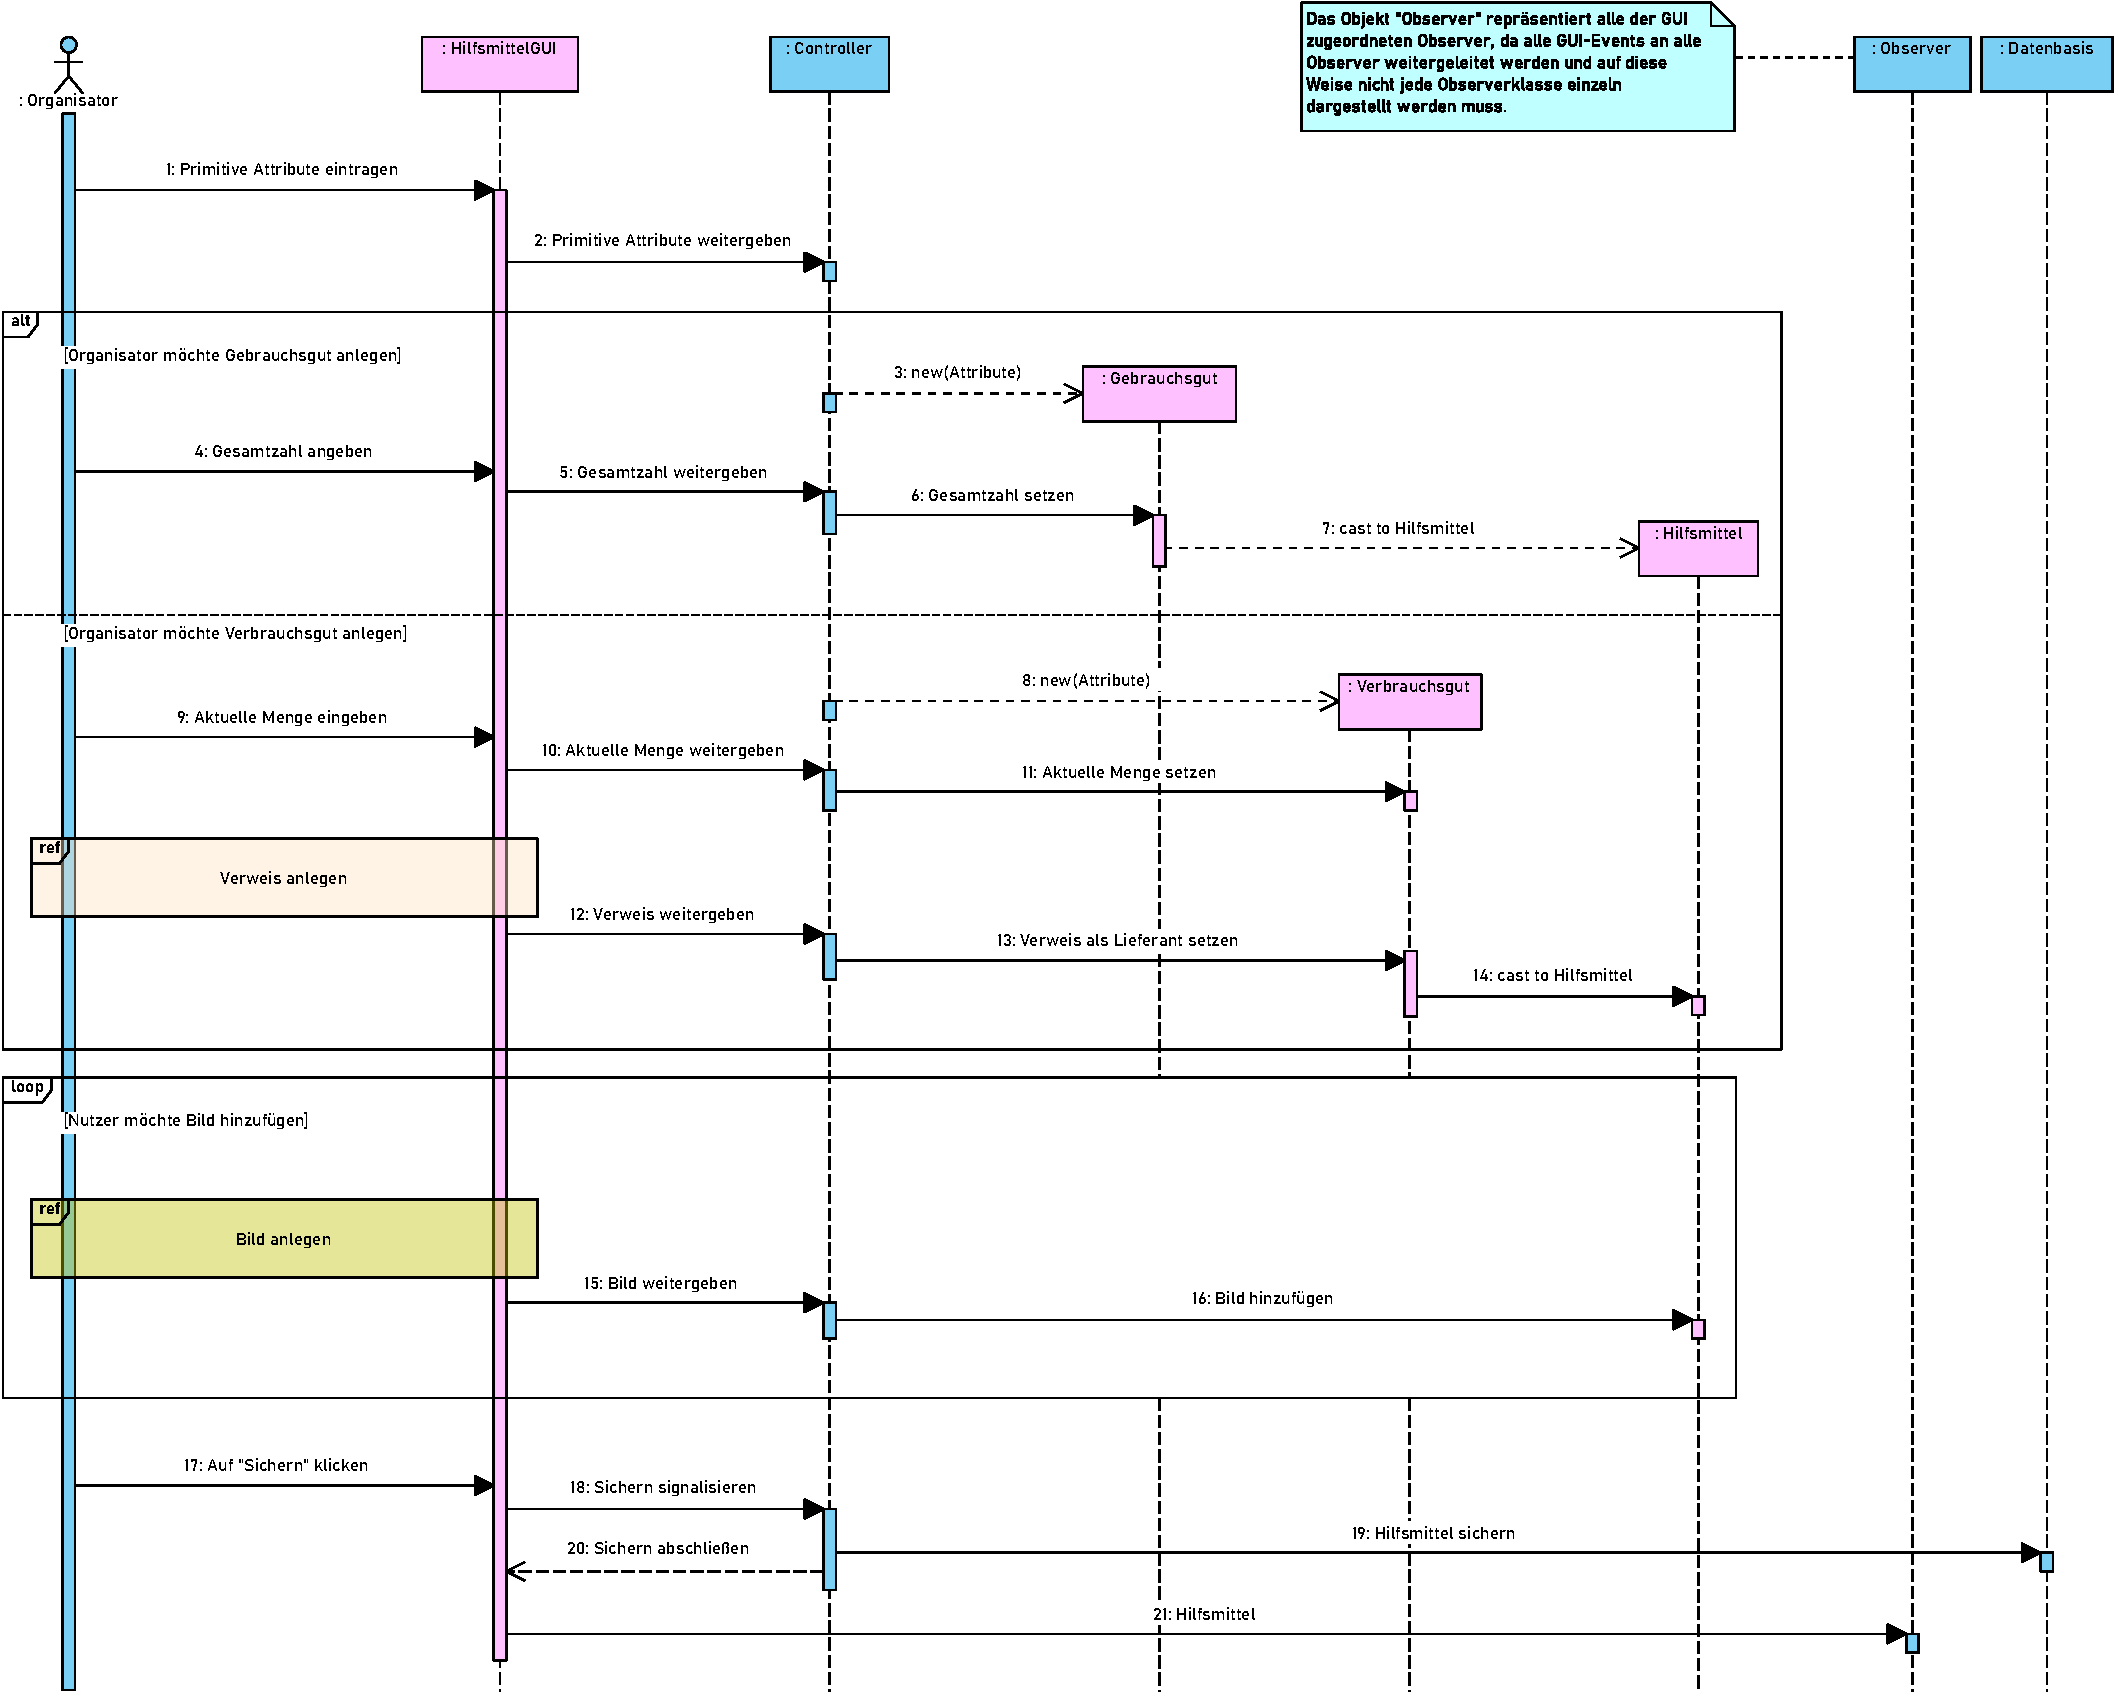
\includegraphics[width=0.98\columnwidth]{Bilder/seq_Hilfsmittel_anlegen.pdf}
    \caption{Szenario Hilfsmittel anlegen}
    \label{seq:hilfsmittel-anlegen}
\end{figure}

Wie man in \autoref{seq:hilfsmittel-anlegen} erkennen kann, trägt der Organisator beim anlegen eines Hilfsmittels zunächst die primitiven Attribute des Hilfsmittels ein. Nun gibt es zwei in einem alt-Fragment dargestellte Pfade: Handelt es sich bei dem anzulegenden Hilfsmittel um ein Gebrauchsgut, so gibt der Organisator zunächst die Gesamtzahl an. Dann wird ein neues Gebrauchsgutobjekt erzeugt, welches zu einem Hilfsmittelobjekt gecastet wird. Handelt es sich um ein Verbrauchsgut, so gibt der Organisator die aktuelle Menge ein, sodass ein Verbrauchsgutobjekt erzeugt werden kann. Nun wird mittels einer Interaktionsreferenz das Sequenzdiagramm \enquote{Verweis anlegen} aufgerufen. Der entstandene Verweis wird dann dem Verbrauchsgutobjekt als Lieferant hinzugefügt und das Verbrauchsgutobjekt zu einem Hilfsmittelobjekt gecastet. Zuletzt hat der Organisator die Möglichkeit dem Hilfsmittel Bilder hinzuzufügen. Hierzu wird innerhalb eines loop-Fragments zunächst das Sequenzdiagramm \enquote{Bild anlegen} aufgerufen und das angelegte Bild dann dem Hilfsmittelobjekt hinzugefügt. Abschließend wird das Hilfsmittel gesichert und auf die Datenbasis geschrieben. 

\include{Inhalt/04_Inhalt/Aktivitätsdiagramm}
\chapter{Entwurfsklassendiagramm}
In diesem Kapitel wird das Entwurfsklassendiagramm erläutert. Es basiert im Wesentlichen auf dem Analyseklassendiagramm, allerdings wurden zusätzlich zu den im Analyseklassendiagramm identifizierten Klassen noch weitere für die Umsetzung nötige Elemente eingeführt und eine Einteilung in Pakete vorgenommen. Im Sinne der Übersichtlichkeit wurden im Entwurfsklassendiagramm statt der einzelnen Klassen die Packages eingefärbt. Lediglich die Klassen, welche persistiert werden sollen und darum das Interface \enquote{IPersistable} implementieren, wurden gelb eingefärbt. Es wird zunächst das Paket \enquote{model} beschrieben bzw. dessen Unterpakete, welche die Klassen aus dem Analyseklassendiagramm enthalten, gefolgt von den Packages der mit dem Entwurfsklassendiagramm eingeführten Klassen. Abschließend werden die im Entwurfsklassendiagramm verwendeten Entwurfsmuster beschrieben.
\FloatBarrier
\begin{figure}[ht!]
    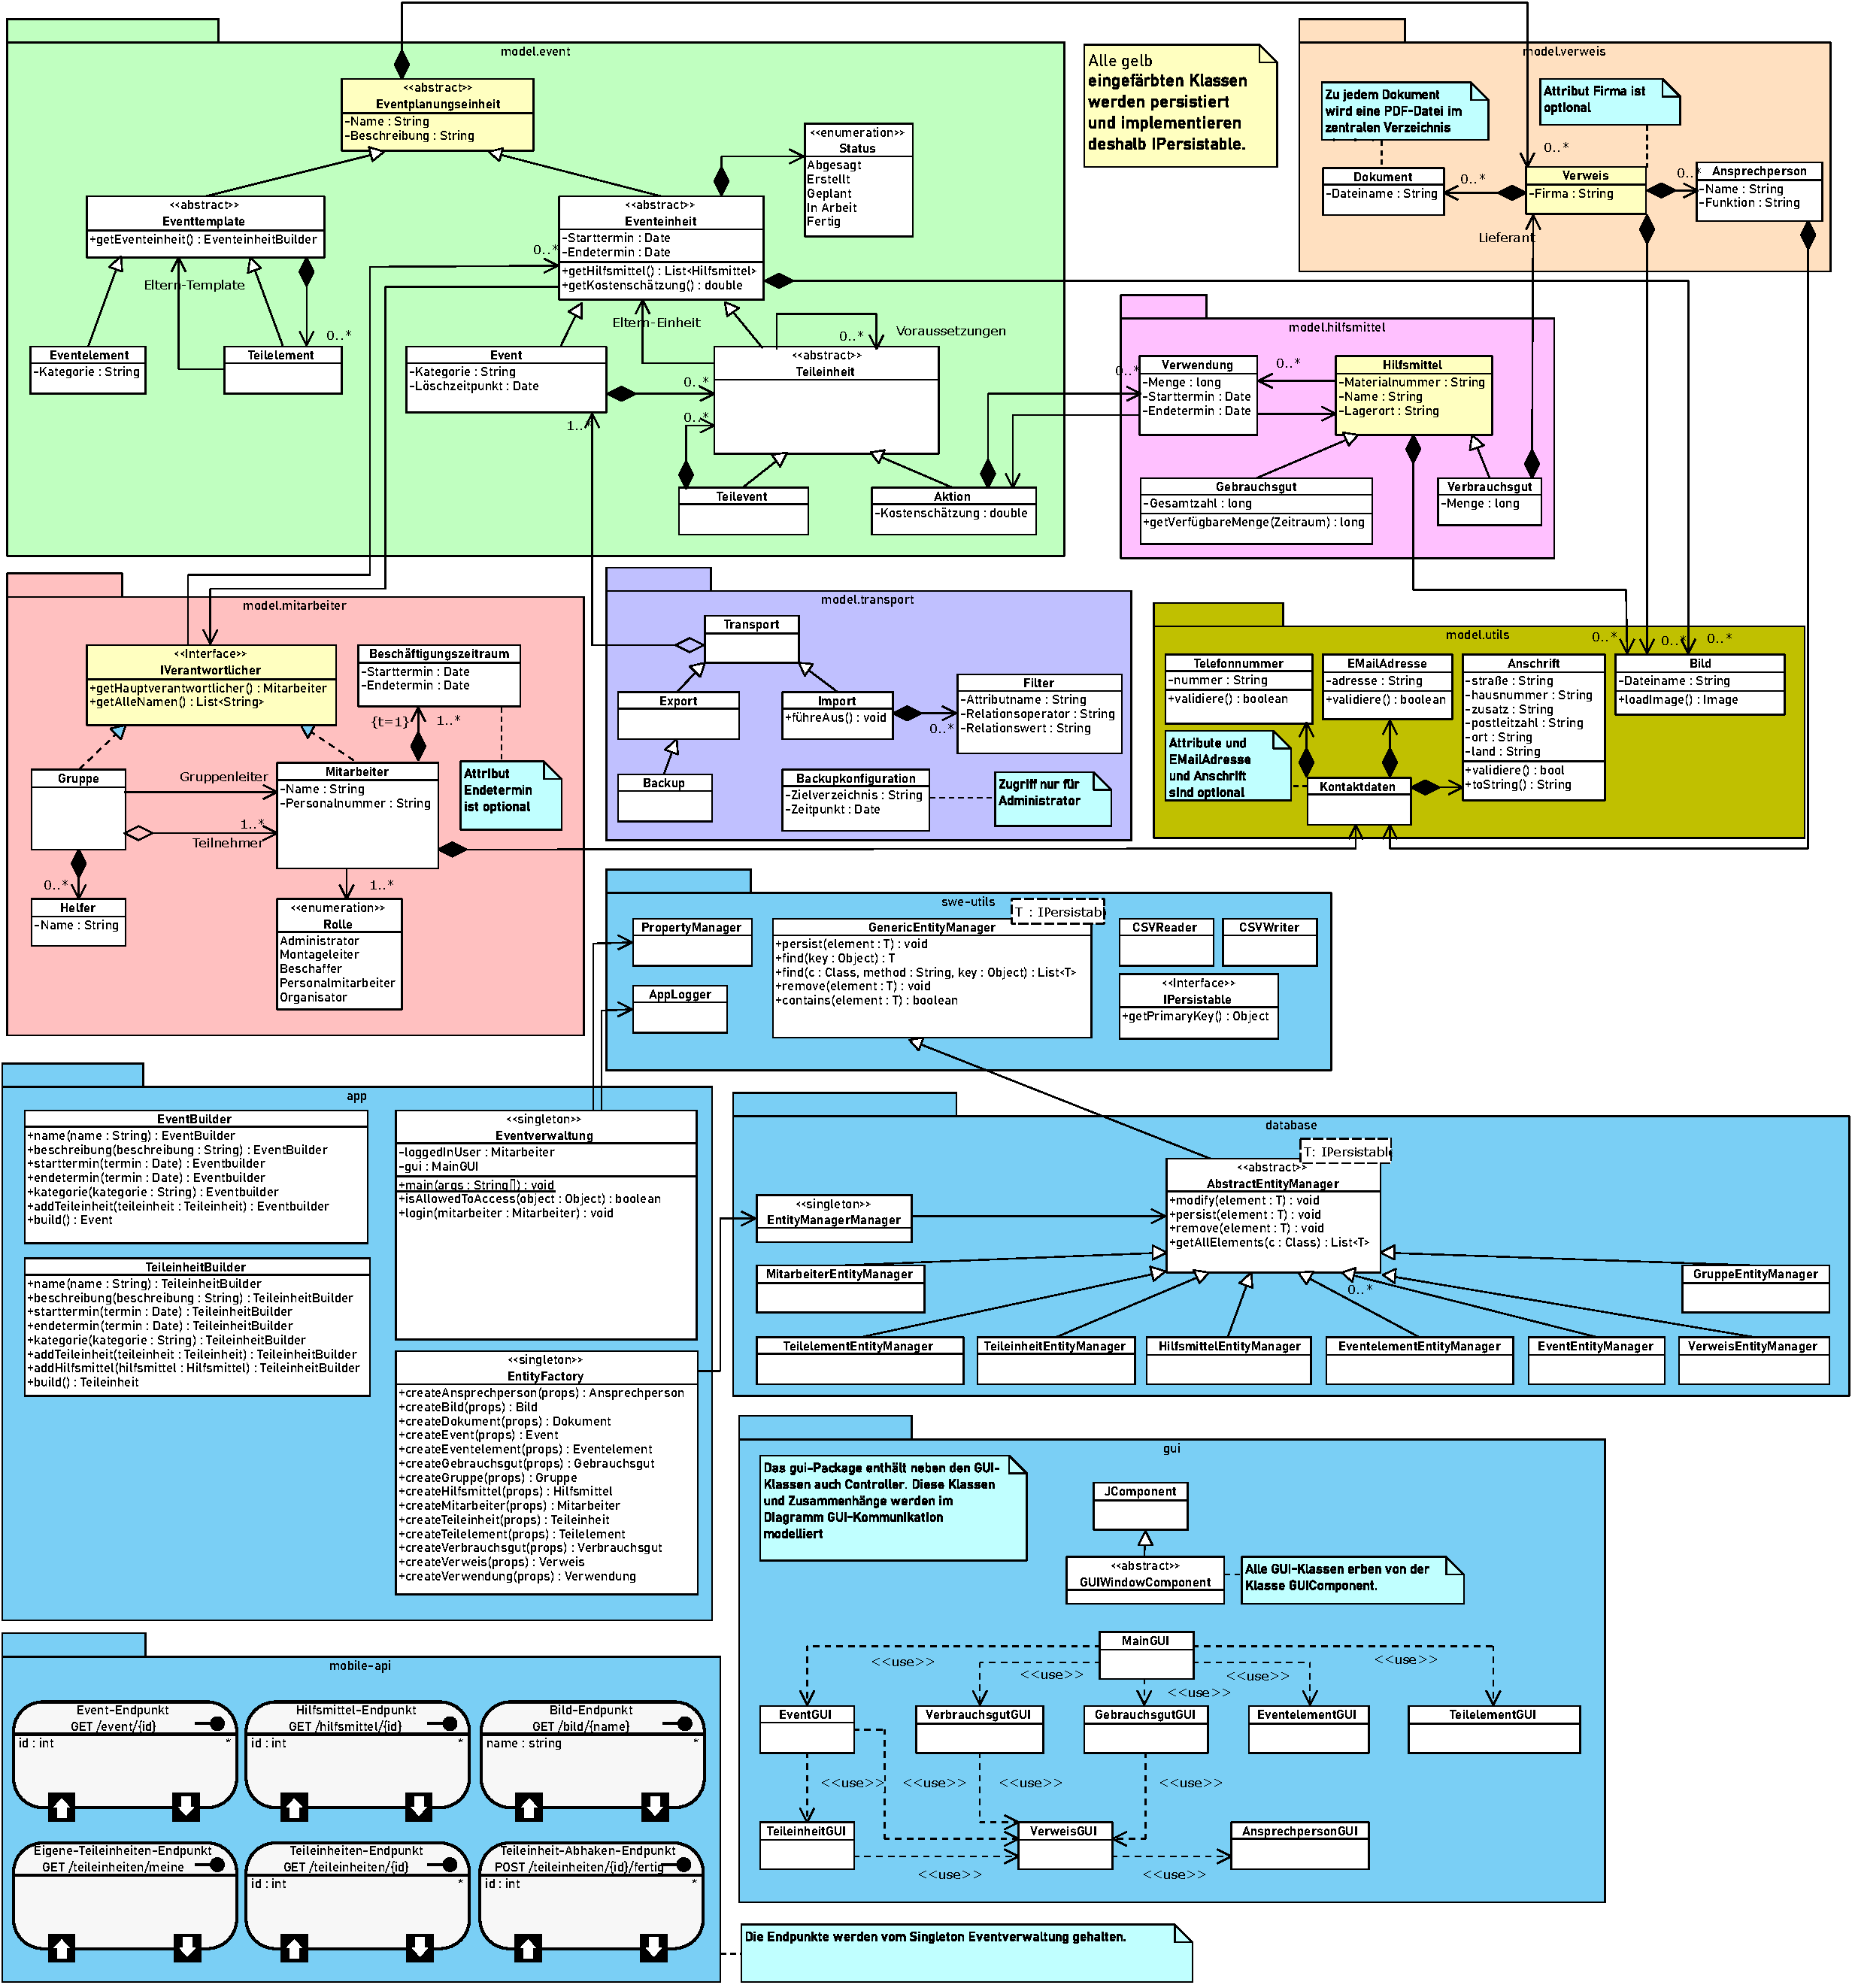
\includegraphics[width=0.98\columnwidth]{Bilder/ekd.pdf}
    \caption{Entwurfsklassendiagramm der Eventplanungssoftware}
\end{figure}

\section{Pakete}

\subsection{model.event}
Dieses Paket enthält alle Klassen aus dem Analyseklassendiagramm, welche Events, Teileinheiten und deren jeweilige Templates betreffen. Da es möglich sein soll, die Events bis zu 14 Tage nach dem Löschen wiederherzustellen, wird ein Event zunächst nur als zu löschend markiert und versteckt. Erst nach 14 Tagen wird es  endgültig aus der Datenbasis gelöscht. Wie man sieht, sind die Klassen Eventplanungseinheit, Eventtemplate sowie Eventplanungseinheit nun abstrakt, da diese nicht instanziiert werden sollen und lediglich der strukturierung der Klassenhierarchie dienen. Ferner sind die Status nun nicht mehr als Unterklassen einer Superklasse \enquote{Status} modelliert, sondern als Enumeration. Die Klasse Teileinheit ist nun ebenfalls abstrakt, da sie nun als Superklasse der Klassen \enquote{Aktion} und \enquote{Teilevent} dient. Diese Unterscheidung ist notwendig, da den Teilevents, welche weitere ihnen untergeordnete Kinderteilevents besitzen, keine Hilfsmittel zugeordnet werden dürfen. Ebenso dürfen den Aktionen, welche Hilfsmittel besitzen dürfen, keine Kinderteileinheiten untergeordnet werden. Darum besitzt nun nur noch die Klasse \enquote{Teilevent} eine Rückassoziation auf die Teileinehit und nur noch die Klasse \enquote{Aktion} eine Assoziation zu \enquote{Verwendung}. Es können jedoch weiterhin beiden Arten von Teilevents weitere Teileinheiten als Voraussetzungen zugeordnet werden.

\subsection{model.verweis}
Dieses Paket enthält neben der Klasse \enquote{Verweis} lediglich \enquote{Dokument} und \enquote{Ansprechperson}, da diese die wesentlichen Bestandteile eines Verweises bilden. Diese konnten vollständig aus dem Analyseklassendiagramm übernommen werden.

\subsection{model.hilfsmittel}
In diesem Paket befinden sich alle Klassen, welche Hilfsmittel sowie deren Zuordnung zu Aktionen betreffen. Die eigentlichen Klassen konnten komplett aus dem Analyseklassendiagramm übernommen werden. Lediglich die Klasse \enquote{Verwendung} besitzt nun nicht mehr eine Assoziation zu der nun abstrakten Klasse \enquote{Teileinheit}, sondern zur Klasse \enquote{Aktion}.

\subsection{model.transport}
Auch die Klassen dieses Paketes, welche den gesamten Datenimport- und export abbilden, konnten vollständig aus dem Analyseklassendiagramm übernommen werden. Um die Übertragung der vorhandenen Eventdaten aus den Excel-Tabellen zu realisieren, wurde keine zusätzliche Funktionalität eingeplant, da diese manuell erfolgen wird.

\subsection{model.mitarbeiter}
Dieses Paket enthält alle Klassen, welche die Verwaltung der Mitarbeiter und deren Zuordnung zu Gruppen betreffen. Hier wurde die Klasse \enquote{Verantwortlicher} in ein Interface umgewandelt, welches von den Klassen \enquote{Gruppe} und \enquote{Mitarbeiter} implementiert wird. Ferner wurden, ähnlich den Status, die Benutzerrollen zu einer Enumeration zusammengefasst, statt sie als einzelne Klassen mit einer Superklasse zu modellieren.

\subsection{model.utils}
In diesem Paket wurden alle Klassen zusammengefasst, welche in mehreren der zuvor beschriebenen Pakete Verwendung finden und darum nicht eindeutig zugeordnet werden konnten. Konkret handelt es sich um die Klassen \enquote{Bild} und \enquote{Kontaktdaten} sowie \enquote{Telefonnummer}, \enquote{EMailAdresse} und \enquote{Anschrift} als Bestandteile der Kontaktdaten.

\subsection{app}
Im Paket \enquote{app} befindet sich zum einen die zentrale Klasse \enquote{Eventverwaltung} mit der Main-Methode zum Starten der Anwendung, welche als Singleton implementiert wird. Sie hält außerdem den \enquote{AppLogger} und den \enquote{PropertyManager} der Anwendung. Ferner befindet sich in diesem Paket das Singleton \enquote{EntityFactory}, eine Fabrikklasse zur Erzeugung von Instanzen derjenigen Klassen, welche in der Datenbasis persistiert werden können. Für die beiden komplexen Klassen \enquote{Event} und \enquote{Teileinheit} existieren in dem Paket außerdem die entsprechenden Builderklassen.

\subsection{database}
Das zentrale Element dieses Paketes ist die abstrakte Klasse \enquote{AbsractEntityManager}, welche von der Klasse \enquote{GenericEntityManager} aus den swe-utils erbt. Der \enquote{AbstractEntityManager} bildet die Superklasse aller konkreten Entity Manager für die zu persistierenden Klassen. Instanziiert und gehalten werden diese durch den \enquote{EntityManagerManager}.

\subsection{gui}
In diesem Paket befinden sich alle Klassen, welche die Benutzeroberfläche betreffen. Die Klassen mit der Endung \enquote{GUI} bilden die Views der Benutzeroberfläche und erben alle von der abstrakten Klasse \enquote{GUIComponent}, welche wiederum von \enquote{JComponent} erben. Die Vererbungspfeile von den Viewklassen zu \enquote{GUIComponent} wurden im Sinne der Übersichtlichkeit nicht dargestellt. Im nachfolgenden Kapitel wird näher auf die Klassen der Benutzeroberfläche eingegangen.

\subsection{swe-utils}
Hier wird lediglich ein Auszug des gesamten Paketes \enquote{swe-utils} dargestellt, nämlich diejenigen Klassen und Interfaces, welche für dieses Projekt verwendet wurden. Dies sind neben den bereits in anderen Paketen erwähnten Klassen, der \enquote{CSVReader} sowie der \enquote{CSVWriter}, welche in den Entity Managern für die Persistierung der Daten verwendet werden. Auch das zu Beginn des Kapitels erwähnte Interface \enquote{IPersistable} stammt aus diesem Paket.

\subsection{mobile-api}
Dieses Paket enthält REST-Endpunkte zum Abfragen von Events, Teileinheiten, Hilfsmitteln und Bildern, außerdem einen separaten Endpunkt zum Abfragen der Teileinheiten, welche einem bestimmten Mitarbeiter zugeordnet sind und schließlich einen Endpunkt zum \enquote{abhaken} abgeschlossener Teileinheiten. Diese bilden die Grundlage der späteren Mobile App in der zweiten Ausbaustufe der Software und werden darum in der jetzigen Phase des Projekts nicht implementiert.

Jeder Endpunkt geht davon aus, dass ein eingeloggter Nutzer die Anfrage stellt und damit in einem Cookie die Session gespeichert ist. Dadurch kann festgestellt werden, welcher Nutzer eingeloggt ist und somit auf welche Objekte zugegriffen werden kann und auf welche nicht.

Die Endpunkte erhalten jeweils Anfrageparameter als Teil der URL und senden Antworten in JSON. Die einzelnen Parameter und Antworten werden im Folgenden näher erläutert, dabei sind die URL-Parameter jeweils in geschweiften Klammern dargestellt. Die Antworten sind schematisch als TypeScript-Objekt angegeben, Referenzen auf andere Elemente haben dabei jeweils den Typen des Primärschlüssels des referenzierten Objektes.
\newpage
\begin{longtable}{l|c|l}
    Endpunkt & Parameter & Antwort \\
    \hline
    GET /event/\{id\} & ID des Events & \begin{lstlisting}[style=json-web-schnittstelle]
{
 id: number,
 name: string,
 beschreibung: string,
 starttermin: Date,
 endetermin: Date,
 verantwortlicher: {
  personalnummer: string,
  name: string
 },
 teilelemente: number[],
 bilder: string[],
 verweise: {
  firma: string?,
  dokumente: File[],
  ansprechpersonen: {
   name: string,
   funktion: string,
   eMailAdresse: string,
   telefonnummer: string,
   anschrift: {
    straße: string,
    hausnummer: string,
    zusatz: string,
    postleitzahl: string,
    ort: string,
    land: string
   }
  }[] 
 }[],
 kategorie: string,
 status: string
}
\end{lstlisting} \\
    \hline
    GET /hilfsmittel/\{id\} & Materialnummer des Hilfsmittels & \begin{lstlisting}[style=json-web-schnittstelle]
{
 materialnummer: string,
 name: string,
 lagerort: string,
 typ: string
}
    \end{lstlisting} \\
    \hline
    GET /bild/\{name\} & Dateiname des Bildes & File \\
    \hline
    GET /teileinheiten/meine & - & \begin{lstlisting}[style=json-web-schnittstelle]
{
    teileinheiten: number[]
}
    \end{lstlisting}\\
    \hline
    GET /teileinheiten/\{id\} & ID der Teileinheit & \begin{lstlisting}[style=json-web-schnittstelle]
{
 id: number,
 name: string,
 beschreibung: string,
 starttermin: Date,
 endetermin: Date,
 verantwortlicher: {
  personalnummer: string,
  name: string
 },
 teilelemente: number[],
 bilder: string[],
 verweise: {
  firma: string?,
  dokumente: File[],
  ansprechpersonen: {
   name: string,
   funktion: string,
   eMailAdresse: string,
   telefonnummer: string,
   anschrift: {
    straße: string,
    hausnummer: string,
    zusatz: string,
    postleitzahl: string,
    ort: string,
    land: string
   }
  }[] 
 }[],
 status: string,
 eltern: number,
 voraussetzungen: number[],
 hilfsmittel: {
  materialnummer: string,
  menge: number
 }[]
}
    \end{lstlisting}\\
    \hline
    POST /teileinheiten/\{id\}/fertig & - & - \\
\end{longtable}

\section{Entwurfsmuster}
Entwurfsmuster sind bewährte wiederverwendbare Vorlagen für die Lösung häufig auftretender Probleme beim Entwurf von Softwaresystemen. Diese Muster haben den Vorteil, dass sie viele bekannte Probleme lösen. In unserer Eventplanungssoftware verwenden wir einige solche Muster, die im Folgenden beschrieben werden.
\subsection{EntityFactory}
Um einzelne Instanzen der Klassen zu erstellen, wird mit der EntityFactory das Muster der EntityFactory umgesetzt. Diese hat eine Methode zum Erstellen eines jeden Objektes und gibt jeweils nach Persitierung im entsprechenden EntityManager eine Instanz des Objektes zurück. Der Übersichtlichkeit wegen wurden die einzelnen Attribute im Diagramm mit \enquote{props} abgekürzt dargestellt. Die EntityFactory ist auch als Singleton modelliert.
\subsection{Singleton}
Im Entwurf sind mehrere Singletons zu finden, dazu gehören die Eventverwaltung, die EntityFactory, der EntityManagerManager und der GUIController. Dadurch soll garantiert werden, dass jeweils nur eine Instanz der Klasse vorhanden ist. Der Sinn dieses Entwurfsmuster ist erkennbar am Beispiel des EntityManagerManagers. Dieser hält eine Instanz des jeweiligen EntityManagers für die spezifische Klasse. Dadurch, dass es immer nur einen EntityManagerManager gibt, ist sichergestellt, dass auch die EntityManager nur einmalig vorhanden sind und somit keine Dateninkonsistenzen auftreten.
\subsection{Builder}
Zum Erstellen der komplexeren Klassen Event und Teileinheit werden Builder bereitgestellt. Damit wird das Objekt Schritt für Schritt erstellt werden und der Zwischenstand stets in dem Builder-Objekt gehalten. Das macht das Erstellen von Event- und Teileinheitobjekten deutlich ergonomischer.
\subsection{Kompositum}
Um die Teil-Ganzes-Hierarchie von Teileinheit zu Unterteileinheiten darzustellen, wird das Kompositum-Muster verwendet. Es wird die Baumstruktur von Teileinheiten, welche Unterteileinheiten besitzen können, abgebildet. Dafür gibt es die Klasse Teileinheit, von welcher Aktion und Teilevent erben. 
\subsection{Beobachter}
Die Beobachter wurden im Entwurf passiv implementiert, daher werden diese lediglich benachrichtigt, wenn Änderungen aufgetreten sind. Die Beobachter fragen nicht aktiv den Zustand des konkreten Subjektes an, da sie das konkrete Subjekt nicht kennen. Dieses ermöglicht eine hohe Abstraktionsmöglichkeit und Wiederverwendbarkeit der einzelnen Komponenten.
\subsection{EntityManager}
Es wurde sich dafür entschieden, konkrete EntityManager pro Klasse zu implementieren, jedoch werden Aktionen und Teilevents sowie Gebrauchsgüter und Verbrauchsgüter jeweils zusammen im TeileinheitEntityManager und HilfsmittelEntityManager verwaltet. Diese Implementierung hat den großen Vorteil, dass die Serialisierung zum Schreiben in CSV-Dateien für jede Klasse einzeln geschrieben werden kann und damit somit weniger Einschränkungen dabei bestehen. Alle konkreten EntityManager erben vom AbstractEntityManager, welcher vom GenericEntityManager aus den swe-utils erbt. Dadurch ist eine gemeinsame Schnittstelle aller EntityManager und trotzdem die Konkretisierung in jeder einzelnen Implementierung vorhanden.

\chapter{GUI-Entwurf}
In diesem Kapitel werden die Komponenten der grafischen Benutzeroberfläche der Eventverwaltungssoftware sowie deren Zusammenspiel erläutert. Auch für die Entwicklung der Benutzeroberfläche wird auf Klassen und Interfaces aus den swe-utils zurückgegriffen, welche im nachfolgenden Abschnitt genauer erläutert werden. Auch die Komponenten der Benutzeroberfläche wurden in Pakete eingeteilt, welche sich an der Struktur der im Entwurfsklassendiagramm modellierten Pakete \enquote{model} orientieren. Deren jeweilige Funktion wird im Anschluss an die Komponenten aus den swe-utils erklärt.

\begin{figure}[ht!]
    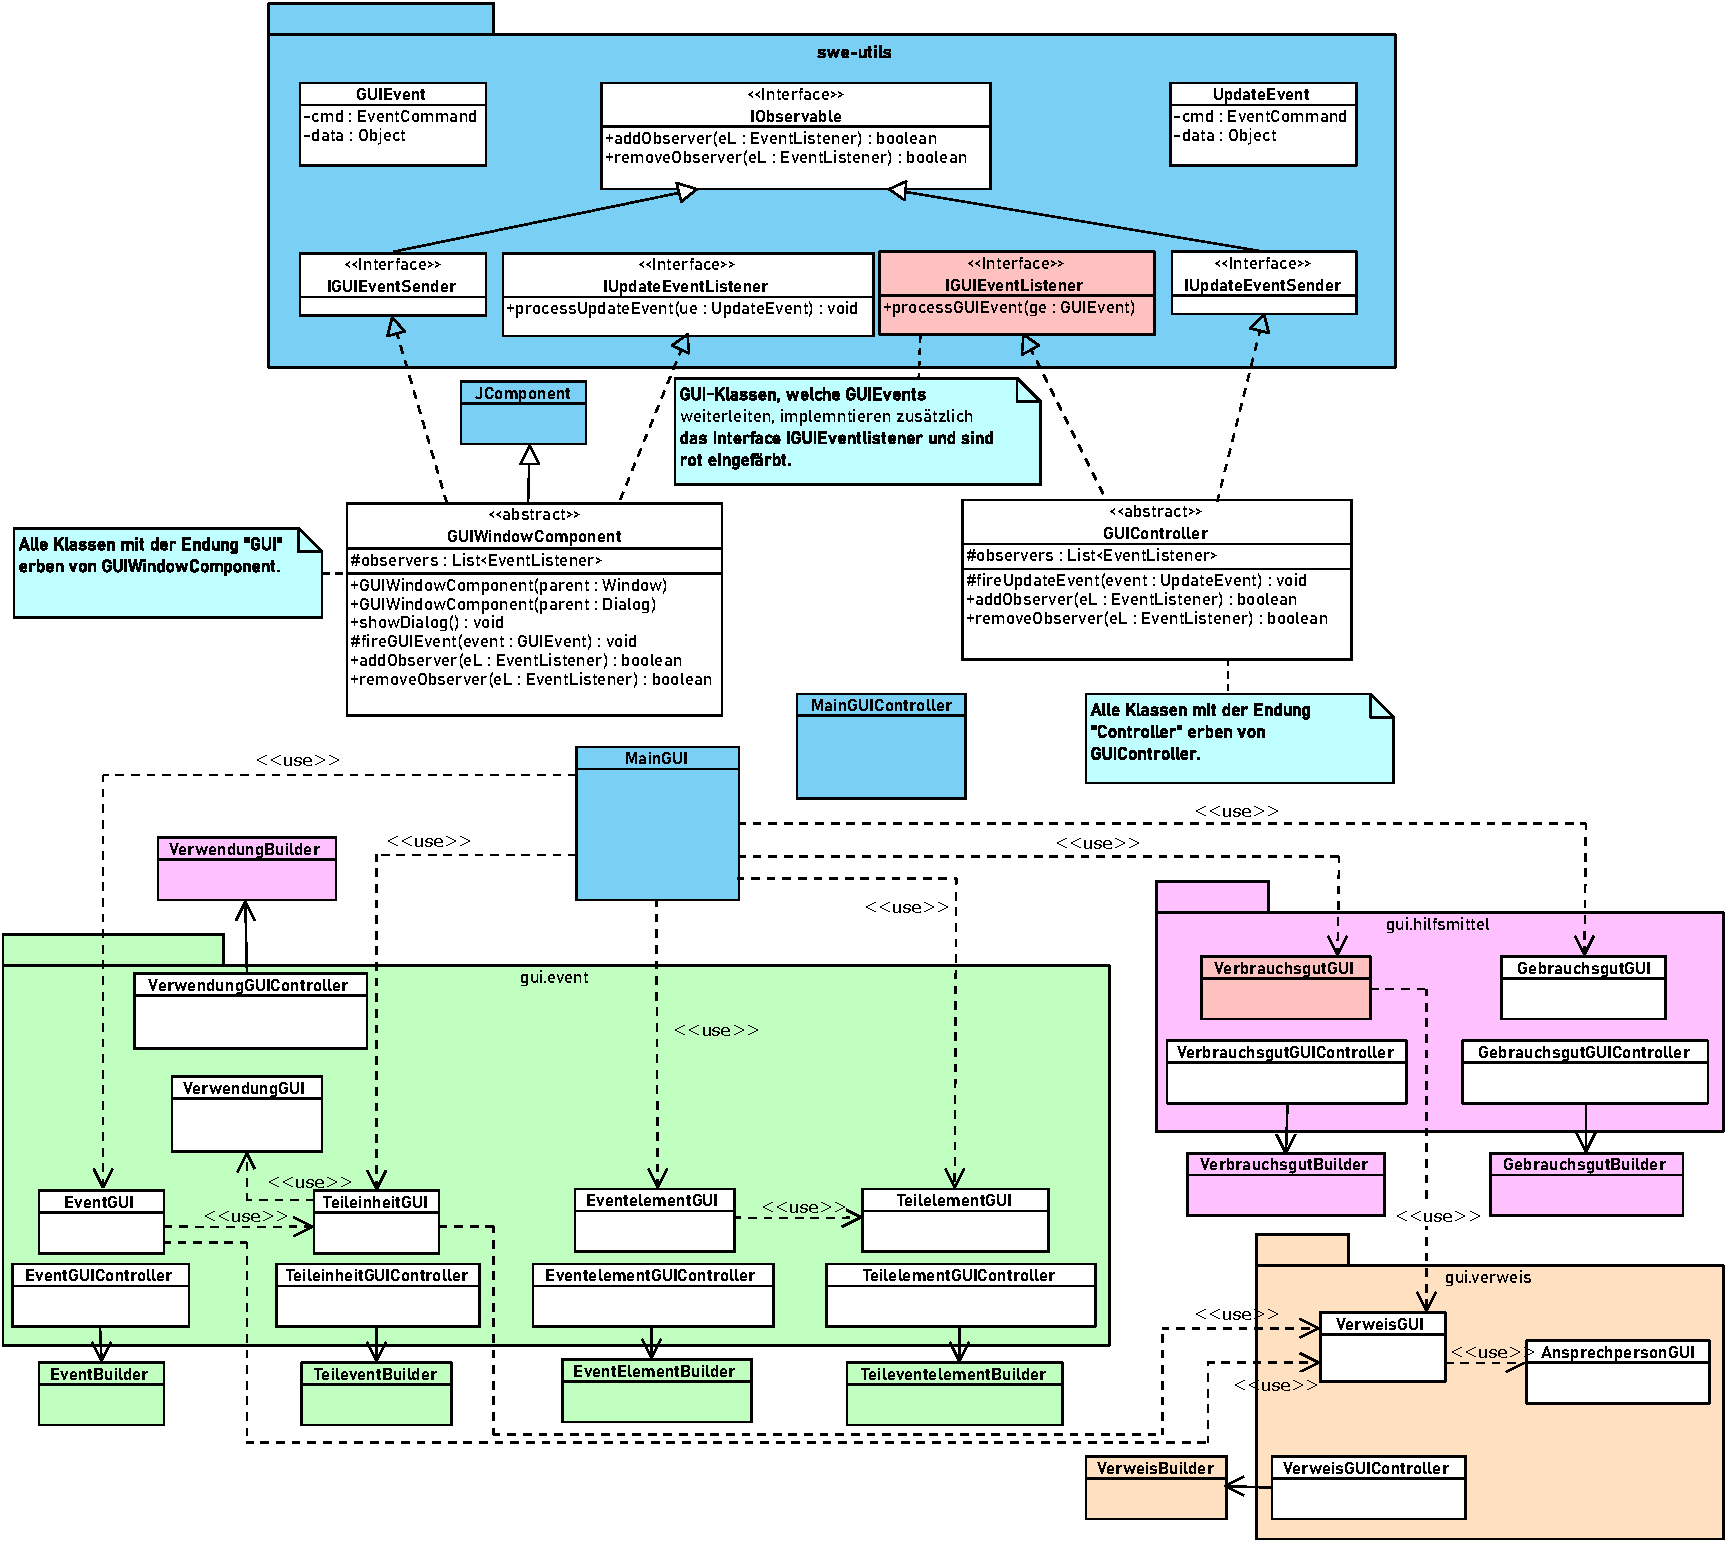
\includegraphics[width=0.98\columnwidth]{Bilder/ekd_GUI.pdf}
    \caption{Entwurfsklassendiagramm der GUI}
\end{figure}

\section{swe-utils}
Als Grundlage des GUI-Entwurfes werden zur Umsetzung des Observerpatterns Interfaces aus den swe-utils verwendet. Für von einem View ausgehende Signale an Controller werden GUIEvents verwendet, für von einem Controller an den View gehende Signale hingegen werden UpdateEvents verwendet. Diese beiden Klassen haben jeweils einen EventCommand und Nutzdaten. Diese Daten sind dabei allgemein gehalten und der EventCommand ist ebenfalls lediglich eine Oberklasse, die von den einzelnen Sender-Klassen mit jeweils einem Commands-Enum erweitert wird.

Die Interfaces \enquote{IGUIEventSender} und \enquote{IGUIEventListener} bilden die Kommunikation von View zu Controller ab. Alle Views erben von \enquote{GUIWindowComponent}, welches \enquote{IGUIEventsender} implementiert und sendet damit GUIEvents an die GUIController, welche \enquote{IGUIEventListener} implementieren.

Entsprechend andersherum ist die Kommunikation von Controller zu View modelliert: Der \enquote{GUIController} implementiert das Interface \enquote{IUpdateEventSender} und sendet damit UpdateEvents an den View, welcher \enquote{IUpdateEventListener} implementiert.

Die beiden Interfaces \enquote{IGUIEventSender} und \enquote{IUpdateEventSender} erben von \enquote{IObservable}, denn sie bilden beide jeweils das Observable im Observerpattern ab. Dafür müssen Methoden zum Hinzufügen und Entfernen von Observern implementiert werden.

Die Klassen \enquote{GUIWindowComponent} und \enquote{GUIController} sind jeweils abstrakte Klassen, von denen die konkreten Views und Controller erben. Sie stellen eine Basis gemeinsamer Funktionalität dar, die das umsetzen des Observerpatterns ermöglicht. Die Klasse \enquote{GUIWindowComponent} erbt dafür von \enquote{JComponent}, welche es ermöglicht, die Views flexibel in einem \enquote{JFrame}, \enquote{JDialog} oder als Komponente in einem \enquote{JPanel} zu verwenden.

\section{Struktur der GUI}
Den Einstiegspunkt der Benutzeroberfläche bildet die \enquote{MainGUI}, welche für jede der Grundfunktionen der Software, wie beispielsweise die Verwaltung von Events, Mitarbeitern oder Hilfsmitteln einen eigenen Tab enthält, welcher wiederum eine tabellarische Übersicht über die vorhandenen Elemente enthält sowie die Möglichkeit, Unter-UIs aufzurufen, um die Elemente detaillierter zu betrachten und zu bearbeiten. 

Das gesamte GUI-Paket besteht aus drei Unterpaketen: Das Paket \enquote{gui.event} enthält alle UI-Komponenten zur Erstellung von Events. Die EventGUI kann hierbei die TeileinheitGUI sowie die VerweisGUI instanziieren, da jedem Event Verweise sowie Teileinheiten hinzugefügt werden können. Die TeileinheitGUI kann ebenfalls die VerweisGUI sowie die VerwendungGUI instanziieren, da für Aktionen auch Hilfsmittel gebucht werden können, was mittels einer Verwendung geschieht.

Das Paket \enquote{gui.event} enthält auch die GUI-Komponenten zur Erstellung von Eventelementen und Teilelementen. Da einem Eventelement auch Teilelemente hinzugefügt werden können, kann die EventelementGUI die TeilelementGUI instanziieren. Das Paket \enquote{gui.verweis} enthält alle notwendigen Komponenten zur Erstellung von Verweisen, hierzu zählt auch das Anlegen von Ansprechpersonen zu einem Verweis, was in einem separaten UI geschieht. 

Die VerweisGUI wird neben den oben beschriebenen GUIs auch von der VerbrauchsgutGUI zum Anlegen von Verbrauchsgütern instanziiert, da zu diesen stets ein Lieferant in Form eines Verweises hinterlegt wird. Diese GUI gehört ebenso wie die GebrauchsgutGUI zum Anlegen von Gebrauchsgütern zum Paket \enquote{gui.hilfsmittel}. Jede der eben beschrieben UIs wird auf Kundenwunsch durch ein eigenes Fenster realisiert.

\section{Kommunikation der GUI-Komponenten}
Da die gesamte Benutzeroberfläche nach dem Model-View-Controller-Pattern entwickelt wurde, existieren zu jeder dieser UIs drei Klassen: Eine Viewklasse, welche die anzuzeigenden UI-Elemente definiert und vom Benutzer ausgelöste Signale in Form von GUIEvents an die jeweilige Controllerklasse weitergibt, bzw. Steuersignale in Form von Update-Events von dieser empfängt. Bei diesen Viewklassen handelt es sich jeweils um die Klassen mit der Endung \enquote{GUI}. Zu jeder Viewklasse existiert außerdem eine Controllerklasse, welche die GUIEvents von den Viewklassen empfängt, verarbeitet und Steuersignale an die Viewklassen sendet. Die Kommunikation zwischen diesen beiden Klassen erfolgt lediglich mittels den eben genannten Events und realisiert damit das Observerpattern. Jeder Controller hält eine Referenz auf eine Builderklasse für die jeweilige Entität. Diese realisiert das Builderpattern und hält die durch den Benutzer eingegeben Daten bis dieser auf den Sichern-Knopf klickt. Dann wird mittels der Builderklasse das entsprechende Objekt gebaut und mit Hilfe der im Entwurfsklassendiagramm beschriebenen EntityFactory und des jeweiligen EntityManagers persistiert.

Eine Ausnahme bildet hier der MainGUIController, welcher als einziger keine Builderklasse referenziert, da die MainGUI keiner bestimmten Entität zugeordnet ist. Außerdem besitzt die AnsprechpersonGUI keinen eigenen Controller, da Ansprechpersonen lediglich bei Verweisen angelegt werden können. Aus diesem Grund wird die AnsprechpersonGUI durch den entsprechenden VerweisGUIController gesteuert. Ferner sind manche der Viewklassen rot eingefärbt, um zu kennzeichnen, dass diese zusätzlich das Interface \enquote{IGUIEventListener} implementieren, da sie GUIEvents untergeordneter GUIs an ihren Controller weiterleiten.

\chapter{Besonderheiten}
\section{Mobile Version}

\FloatBarrier

Im Lastenheft wurde erwähnt, dass es in einer zweiten Ausbaustufe möglich sein soll, Aufgaben auf mobilen Geräten einzusehen und abhaken zu können. Dafür wurde geplant, dass diese mobile Version über eine Schnittstelle mit dem hier entworfenen System kommuniziert und als Mobile-App auf den mobilen Geräten zur Verfügung steht.

Dafür wurden im Entwurf die einzelnen Endpunkte der REST-Schnittstelle spezifiziert und ausdefiniert, über welche die mobile Anwendung alle nötigen Daten senden und empfangen kann. Diese Schnittstelle ist möglichst minimal gehalten, um keine Funktionalität zu implementieren, die nicht weiter benötigt wird.

\begin{figure}[ht!]
    \centering
    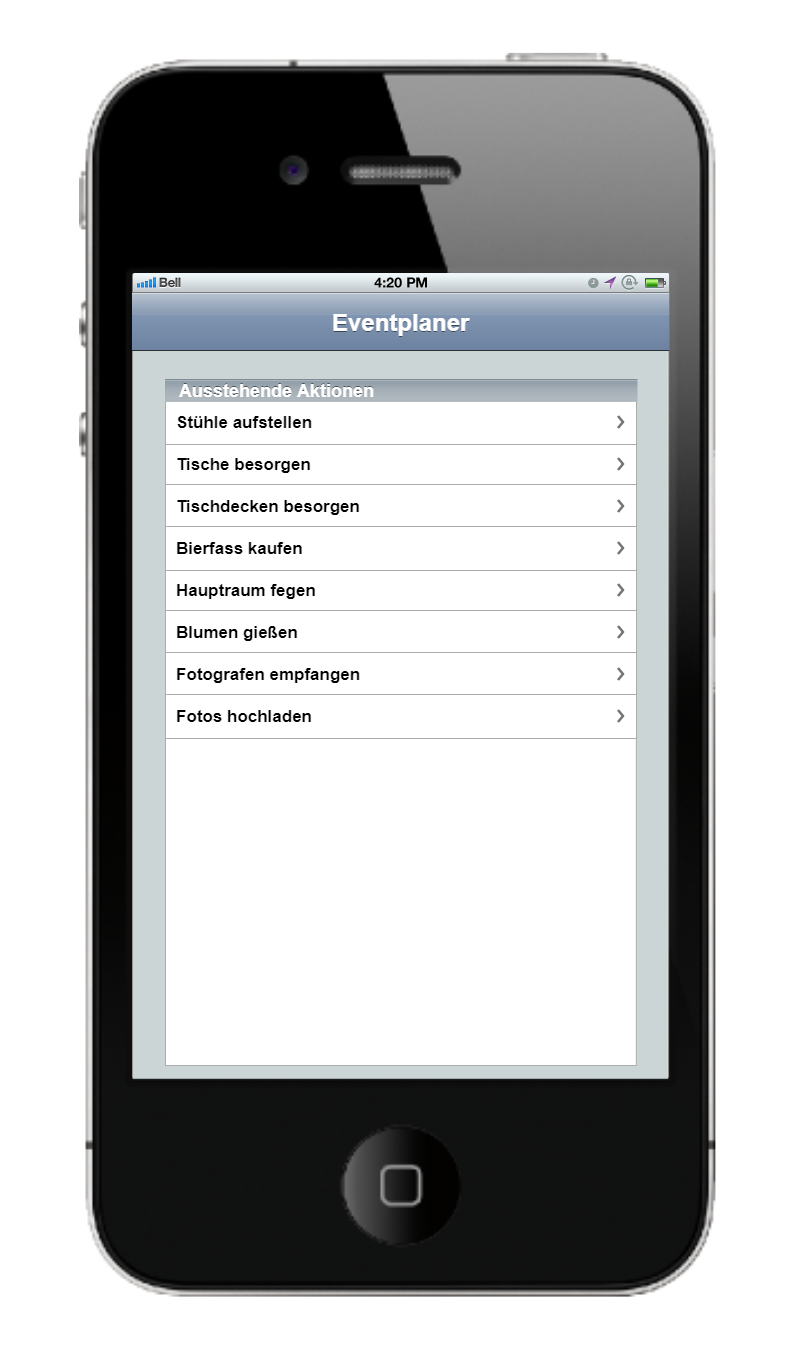
\includegraphics[width=0.4\columnwidth]{Bilder/mockup_mobile_overview.png}
    \caption{Einstiegsansicht der mobilen Version des Eventplaners}
    \label{fig:mockup:mobile:overview}
\end{figure}

In \autoref{fig:mockup:mobile:overview} ist ein Mockup einer Übersichtsseite der geplanten Mobilanwendung zu sehen. Der Nutzer sieht ausschließlich die ihm zugeteilten, ausstehenden Aktionen und kann durch ein Tippen auf eine dieser Aktionen zu den Details gelangen. Hier haben wir darauf geachtet, dem Nutzer eine minimale Benutzeroberfläche zu bieten, um bei der Arbeit mit der Anwendung nicht durch komplizierte Menüs navigieren zu müssen, sondern nur Informationen zu sehen.

\begin{figure}[ht!]
    \centering
    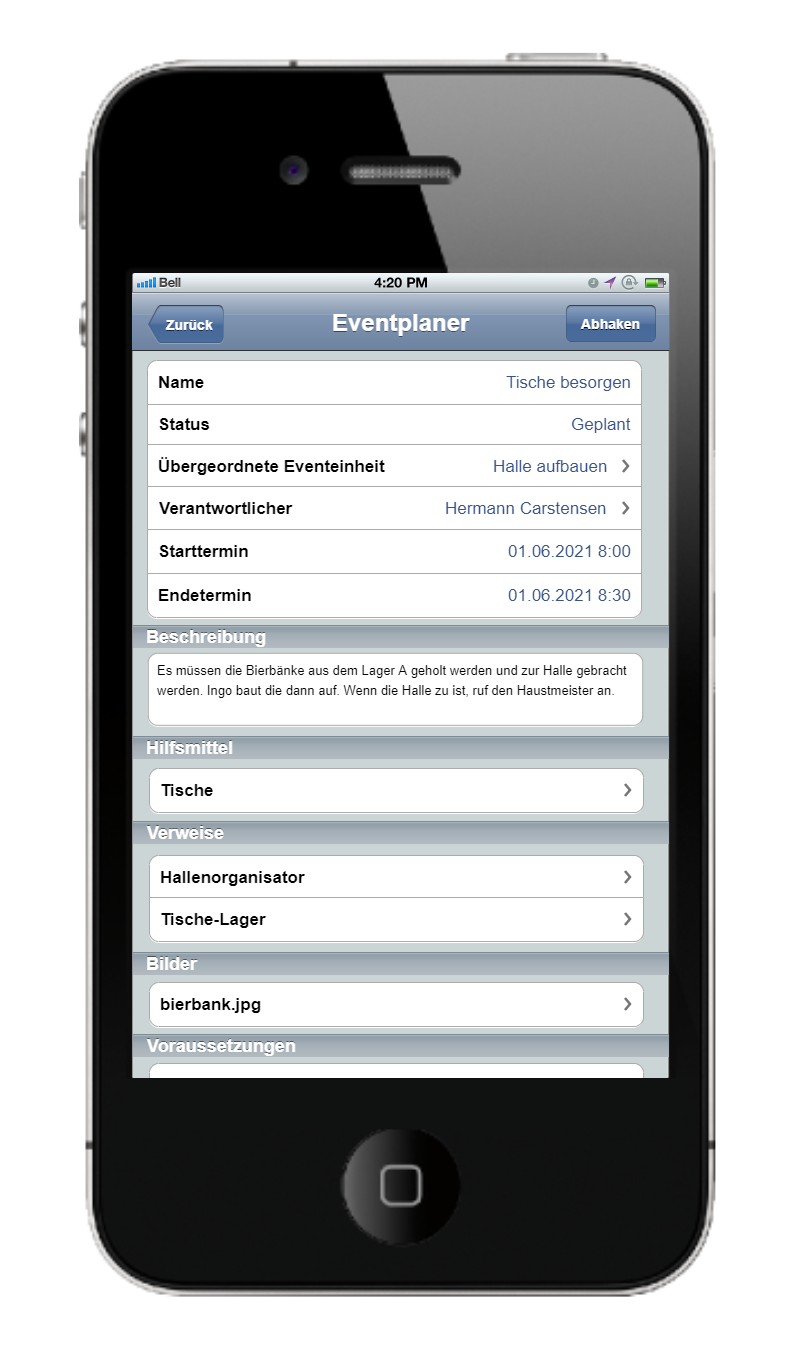
\includegraphics[width=0.4\columnwidth]{Bilder/mockup_mobile_object_page.png}
    \caption{Detailansicht einer Aktion der mobilen Version des Eventplaners}
    \label{fig:mockup:mobile:detail}
\end{figure}

In \autoref{fig:mockup:mobile:detail} ist das Mockup der Detailansicht einer Aktion in der mobilen Version des Eventplaners zu sehen. Hier ist ersichtlich, dass dem Nutzer alle notwendigen Informationen zur Verfügung stehen und jeweils durch ein Tippen auf zugeordnete Elemente wie Hilfsmittel, Verweise und den Verantwortlichen auf die Details dieser Objekte navigiert werden kann. Des Weiteren ist zu sehen, dass in der Kopfleiste der Anwendung zwei Knöpfe vorhanden sind: Links ein Zurück-Knopf, um wieder auf die Übersicht zu gelangen und rechts ein Knopf mit der Aufschrift \enquote{Abhaken}. Durch diesen Knopf kann der Nutzer, da er der Hauptverantwortliche der geöffneten Teileinheit ist, diese Teileinheit in den Status \enquote{Fertig} versetzen.

Damit sind die Anforderungen des Kunden im Mockup der Mobilanwendung sowie durch die Schnittstelle realisierbar und können problemlos in der zweiten Ausbaustufe der Software umgesetzt werden.

\FloatBarrier
\section{Eventtemplates}

Das wesentliche Ziel unserer Software ist es, die Abläufe in den Unternehmen unserer Kunden zu unterstützen und effizienter zu gestalten. Hierzu gehört insbesondere die Vermeidung bzw. Automatisierung trivialer oder repetitiver Tätigkeiten. Gerade repetitive Aufgaben können bei der Eventplanung auftreten, wenn Events gleicher Art, wie beispielsweise mehrere Hochzeiten oder mehrere Kongresse, geplant werden müssen, da hier häufig ähnliche Abläufe und Teileinheiten auftreten. Um nun die Planung ähnlicher Abläufe nicht bei jedem Event händisch durchführen zu müssen, wünschte der Kunde die Möglichkeit, sogenannte Eventelemente verwenden zu können, welche als Vorlagen für Events oder Teileinheiten dienen können. Dieser Gedanke wurde von uns aufgegriffen und noch weiter verfeinert. So kennt unsere Software unter dem Oberbegriff \enquote{Eventtemplates} sowohl \enquote{Eventelemente}, als auch \enquote{Teilelemente}. Wie die Namen bereits vermuten lassen, dienen erstere als Vorlagen für ganze Events, letztere als Vorlagen für einzelne Teileinheiten. Eventelemente können hierbei analog zu Events beliebig viele Teilelemente beinhalten, welche wiederum als Vorlagen für einzelne Teileinheiten dienen. Im Zuge der Modellierung wurde von uns also der im Lastenheft verwendete grobe Begriff \enquote{Eventelemente} aufgebrochen und unterschieden in Vorlagen für Events und Vorlagen für Teileinheiten. Diese Unterscheidung ermöglicht es den Nutzern, spezifischere Vorlagen für bestimmte Anwendungen zu definieren und auf diese Weise bei deren Verwendung noch weniger immergleiche Tätigkeiten ausführen zu müssen.

\section{Gestaltung des Entwurfes mit Fokus auf Flexibilität in der Arbeitsweise}
Da bei der Analyse des Lastenheftes und dem damit einhergehenden Kontakt mit dem Kunden klar wurde, dass dieser möglichst viel Flexibilität beim Umgang mit der Software wünscht. Um dieser Anforderung gerecht zu werden, haben wir an vielen Stellen bewusst Freiheiten gelassen und schränken den Nutzer somit nicht unnötig ein.

Ein Beispiel hierfür ist, dass Mitarbeiter bei uns für mehrere sich überlappende Teileinheiten gleichzeitig verantwortlich sein können. So wird es erfahrenen Mitarbeitern ermöglicht, ihre Zeit zwischen den Aufgaben dynamisch aufzuteilen und der Kunde kann auf diese Weise deren Arbeitserfahrung und Zeitmanagementfähigkeiten optimal nutzen.

Ein weiteres Beispiel ist in der Verwendung vieler Freitextfelder zu sehen. Durch die Vorgabe einer festen Struktur bei Namen, Materialnummern oder Kategorie kann das Unternehmen seine organisatorischen Details ändern, ohne die Software anpassen zu müssen. Dieses Konzept ist auch bei den Verweisen zu sehen, denen Dokumente zugeordnet werden können. Die Software trifft keine Einschränkung in den Dateitypen der zuordenbaren Dokumente, sodass jede Datei einem Verweis zugeordnet werden kann. Dadurch benötigt der Nutzer keine weiteren Verzeichnisse und Anhänge zu Events, sondern kann alle Informationen zum Event direkt in der Software speichern.

Ein letztes Beispiel für diese Flexibilität ist in der Rollenzuweisung ersichtlich. Jeder Nutzer kann eine, mehrere oder alle Rollen besitzen. Dadurch ist gewährleistet, dass jede Verantwortlichkeit innerhalb des Unternehmens gut abgebildet werden kann, wie zum Beispiel ein Personalmitarbeiter, der gelegentlich auch als Montageleiter tätig ist.

Diese Beispiele zeigen, dass wir in unserem Entwurf großen Wert darauf gelegt haben, den Kunden nicht in seiner Arbeitsweise einzuschränken, sondern mit unserer Software zu unterstützen. Die vielen Möglichkeiten der Flexibilität zeigen eine Anpassungsfähigkeit der Software an die Prozesse des Unternehmens und verhindern somit dass kreative Ideen für Prozessoptimierungen an der Softwarekompatibilität scheitern.

\section{Desktoporientierte Benutzeroberfläche}
Um die Möglichkeiten eines Desktop-PCs bei der Darstellung mehrerer Fenster vollends auszunutzen, setzt unsere Software auf Wunsch des Kunden auf die Aufteilung verschiedener Aufgaben in verschiedene Fenster. So wird jede GUI zur Anzeige oder zur Bearbeitung eines Objektes in einem separaten Fenster angezeigt. Diese strukturierte Einteilung unterstützt den Endnutzer nicht nur dabei, die Übersicht über die von ihm Bearbeiteten Objekte mit ihren teilweise komplexen Zusammenhängen zu behalten, sondern ermöglicht es auch, mehrere Objekte zugleich zu öffnen. Dieses Feature ist besonders hilfreich, sollte der Nutzer beispielsweise beim Erstellen einer Teileinheit zusätzliche Informationen, etwa aus einer anderen Teileinheit oder dem übergeordneten Event, benötigen. Durch die Möglichkeit, mehrere Fenster parallel zu öffnen, kann er diese Informationen leicht erhalten, ohne seine eigentliche Arbeit zu unterbrechen und die dafür notwendige Ansicht zu verlassen, wie es bei einer Anwendung mit nur einem einzigen Fenster nötig wäre. Auf diese Weise unterstützt unsere Software aktiv den Workflow der Nutzer und steigert somit deren Produktivität und Motivation.

\section{Unterscheidung in Verbrauchsgut und Gebrauchsgut}
Bereits bei der Analyse des Lastenhefts wiesen wir in einer unserer Fragen darauf hin, dass es sinnvoll wäre, verschiedene Arten von Hilfsmitteln mit unterschiedlichen Attributen zu unterscheiden. Dieser Vorschlag wurde durch den Kunden angenommen und er beauftragte uns, bei der Modellierung der Hilfsmittel zwei verschiedene Arten derselben zu unterschieden: Zum einen die Gebrauchsgüter, welche mehrfach benutzt werden können und dabei der Abnutzung unterliegen, zum anderen die Verbrauchsgüter, welche nach einmaliger Nutzung verbraucht sind und dementsprechend nicht wiederverwendet werden können. 

Der wesentliche Unterschied bei der Verwaltung der beiden Arten von Hilfsmitteln liegt darin, dass für ein Verbrauchsgut lediglich die insgesamt verfügbare Menge gespeichert werden muss. Sobald eine gewisse Stückzahl des Verbrauchsgutes durch eine Verwendung für eine Aktion gebucht wird gilt diese als verbraucht und die im System hinterlegte Menge wird entsprechend reduziert. Aus diesem Grund muss für die schnell aufgebrauchten Verbrauchsgüter ein ständiger Nachschub gewährleistet werden. Um diesen Prozess zu unterstützen, bietet unser System die Möglichkeit, für jedes Verbrauchsgut einen Lieferanten zu hinterlegen. Auf diese Weise können bei knappem Lagerbestand Verbrauchsgüter ohne großen Suchaufwand nachbestellt werden. 

Das Hinterlegen eines Lieferanten ist bei den Gebrauchsgütern nicht notwendig und wurde darum auch nicht von uns umgesetzt, um die Software möglichst einfach und ohne überflüssige Funktionalitäten zu gestalten. Dafür erwies sich die Berechnung der für einen bestimmten Zeitraum verfügbaren Menge eines Gebrauchsgutes vergleichsweise komplex. Durch den Nutzer gepflegt werden muss dennoch lediglich die Gesamtmenge des Gebrauchsgutes, welche der Kunde besitzt. Möchte er nun ein Gebrauchsgut für einen bestimmten Zeitraum für eine Aktion buchen, so wird durch das System automatisch die für den geplanten Zeitraum verfügbare Menge auf Basis der vorhanden Gesamtmenge sowie weiterer Buchungen des Gebrauchsgutes berechnet. Auf diese Weise kann ein Mangel an einem bestimmten Gebrauchsgut frühzeitig erkannt und behoben werden. 

Diese Unterscheidung wurde von uns bereits bei der Entwicklung des Analyseklassendiagramms berücksichtigt und wird auch in der Implementierung umgesetzt werden. Da wir stets mit dem Ziel arbeiten, unsere Software für alle Beteiligten möglichst transparent zu gestalten und darum nach den Methoden des Domain-driven Design arbeiten, wurde selbstverständlich auch die durch den Kunden vorgeschlagene Nomenklatur für die beiden Arten von Hilfsmitteln von der Analyse bis hin zur Implementierung beibehalten. 



% ---- Anhang
\appendix
\clearpage
\pagenumbering{Roman}  % römische Seitenzahlen für Anhang
\setcounter{page}{\numexpr\value{savepage}+1}

\chapter{E-Mails des Auftraggebers}
\begin{figure}[ht!]
    \centering
    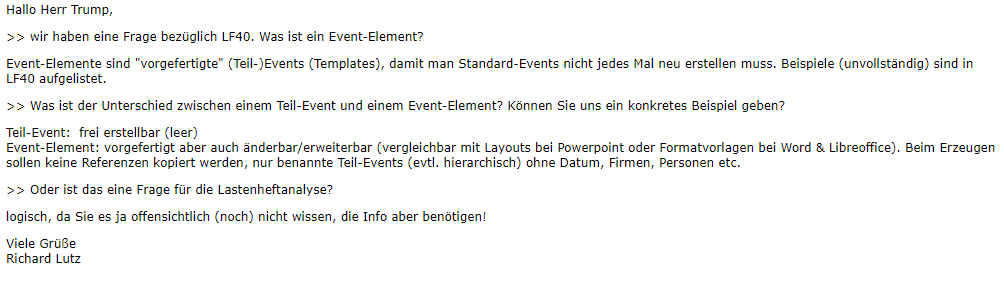
\includegraphics[width=1.0\textwidth]{Bilder/mail_eventelemente.png}
    \caption{Mail des Auftraggebers}
    \label{fig:email:eventelemente}
\end{figure}
In \autoref{fig:email:eventelemente} ist der Screenshot einer Mail des Auftraggebers zu sehen, in welcher die Bedeutung des Begriffes \enquote{Eventelement} im Lastenheft genauer geklärt wird.

\newpage
\end{document}
